\documentclass[a4paper, 12pt, pointlessnumbers]{scrreprt}	    % Dokumenten Klasse
\usepackage[left= 2.5cm,right = 2cm, bottom = 4 cm]{geometry}   % Rand Geometrie
\usepackage[onehalfspacing]{setspace}		                    % Mache nur ein Leerzeichen

\usepackage[utf8]{inputenc}					% Zeichensatz für Umlaute
\usepackage[ngerman]{babel}                 % Zeichensatz für \flqq \frqq
% \usepackage[T1]{fontenc}                   % Schriftart
\usepackage{graphicx}				        % Bilder Packet
\usepackage{float}                          % Bilder positionieren
\usepackage{tikz}                           % Zeichnen
\usepackage{svg}                            % SVG Bilder
\usepackage{url}							% URL im Literaturverzeichnis
\usepackage{scrhack}                         % Fix deprecated \float@addtolist warning with KOMA-Script
\usepackage[hidelinks]{hyperref}            % Links im Dokument
\usepackage{booktabs}                       % Tabellen Linien
\usepackage{color}                          % Text Farben
\usepackage{pgfgantt}                       % Gantt Chart
\usepackage{csvsimple}                      % csv files
\usepackage{longtable}                      % tabellen für api
\usepackage{array}                          % tabellen für api
\usepackage{seqsplit}                       % tabelle api
\hyphenation{De-zi-mal-tren-nung}			% Silbentrennung
\hyphenpenalty=9750							% Weniger Silbentrennung
\usepackage{csquotes}
\usepackage[backend=biber, style=numeric, url=true, sorting=none]{biblatex}
\addbibresource{quellen.bib}
\usepackage[acronym, toc]{glossaries}
\makeglossaries
\loadglsentries{content/acronyms}
\usepackage{tabularx}
\usepackage{amssymb}
\let\orgautoref\autoref
\renewcommand{\autoref}[1]{(\orgautoref{#1})}

\renewcommand*\chapterheadstartvskip{\vspace*{0.8\topskip}}		% Weniger Platz über Chapter Überschrift

\usepackage{pdflscape}
\usepackage{env}
\usepackage{minted}
% --- Globale Minted (Code-Block) Einstellungen ---

\setminted{
    linenos=true,           % Zeilennummern links anzeigen
    frame=single,           % Ein durchgehender, einfacher Rahmen um den Code
    framesep=2.5mm,         % Abstand vom Rahmen zum Text
    fontsize=\footnotesize, % Die Schrift etwas kleiner machen
    breaklines=true,        % Automatische Zeilenumbrüche
    baselinestretch=1.1,    % Etwas mehr Zeilenabstand für bessere Lesbarkeit
    tabsize=2               % Tabs werden als 2 Leerzeichen gerendert
}
% ==========================================
% SETUP: Pakete für Autorenzuordnung und Todos
% ==========================================
\usepackage{etoolbox}
\usepackage{xparse}
\usepackage[colorinlistoftodos, textsize=tiny, german]{todonotes} % Für To-Do Notizen

% Speicher für die Autorenliste
\newcommand{\authorlist}{}

% --- Makros für die Gliederungsebene ---

\NewDocumentCommand{\authorchapter}{ o m m }{%
    \IfNoValueTF{#1}{%
        \chapter{#2}%
    }{%
        \chapter[#1]{#2}%
    }%
    % NEU: Hier wird die *aktuelle* Nummer fest in die Liste geschrieben
    \edef\doappend{%
        \noexpand\gappto\noexpand\authorlist{\thechapter & \unexpanded{#2} & \unexpanded{#3} \noexpand\\ \noexpand\hline}%
    }%
    \doappend
}

\NewDocumentCommand{\authorsection}{ o m m }{%
    \IfNoValueTF{#1}{%
        \section{#2}%
    }{%
        \section[#1]{#2}%
    }%
    \edef\doappend{%
        \noexpand\gappto\noexpand\authorlist{\thesection & \unexpanded{#2} & \unexpanded{#3} \noexpand\\ \noexpand\hline}%
    }%
    \doappend
}

\NewDocumentCommand{\authorsubsection}{ o m m }{%
    \IfNoValueTF{#1}{%
        \subsection{#2}%
    }{%
        \subsection[#1]{#2}%
    }%
    \edef\doappend{%
        \noexpand\gappto\noexpand\authorlist{\thesubsection & \unexpanded{#2} & \unexpanded{#3} \noexpand\\ \noexpand\hline}%
    }%
    \doappend
}

\NewDocumentCommand{\authorsubsubsection}{ o m m }{%
    \IfNoValueTF{#1}{%
        \subsubsection{#2}%
    }{%
        \subsubsection[#1]{#2}%
    }%
    \edef\doappend{%
        \noexpand\gappto\noexpand\authorlist{\thesubsubsection & \unexpanded{#2} & \unexpanded{#3} \noexpand\\ \noexpand\hline}%
    }%
    \doappend
}

\begin{document}
% \begin{singlespace}
    \parindent 0pt % Kein hängender Einzug
    
    \pagenumbering{Roman}
    \begin{titlepage}
    \begin{center}
        % Logo mittig oben
        
\includegraphics[height=6cm]{content/bilder/logo_bulme.png}\\[2cm]
    
        \centering
        {\LARGE Diplomarbeit }\\[1cm]
        {\LARGE EffSync}\\[1cm]
        \includesvg[height=6cm]{content/bilder/EffSync.svg}\\[2cm]
        {\large Entwicklung und Implementierung eines webbasierten Taskmanagementsystems zur effizienten Organisation und Zusammenarbeit in Teams}\\[0.8cm]
        {\large 3/4AKIFT }\\[0.8cm]
        {\large Drazen Plavsic und Ereny Micail}\\[3cm]
        {\large \today}
    \end{center}
\end{titlepage}
    \tableofcontents
    \newpage
    \pagenumbering{arabic}
    
    \authorchapter{Einleitung}{Ereny Micail}

Wer kennt das nicht: In der Schule oder im Team läuft alles über verschiedene Apps.
Aufgaben hier, Nachrichten dort, Dateien woanders.
Nach ein paar Wochen weiß keiner mehr, was Sache ist.
Das nennt man \textit{Context Switching} -- und es kostet nicht nur Zeit, sondern
sorgt auch dafür, dass Infos verloren gehen und keiner mehr weiß, wer für was
zuständig ist.

Genau das wollten wir mit \textit{EffSync} lösen.
\textit{EffSync} ist eine Webanwendung, die Aufgabenverwaltung und Chat in einem
System zusammenbringt -- alles an einem Ort, kein Hin- und Herwechseln mehr.
Nutzer können Tasks anlegen, zuweisen und verfolgen, und gleichzeitig direkt im
Projekt-Kontext miteinander schreiben.
Das Ziel der Arbeit war, genau das umzusetzen und zu zeigen, dass es funktioniert.
Dabei haben wir drei Dinge in den Mittelpunkt gestellt: eine saubere Task-Struktur
mit klaren Berechtigungen, Echtzeit-Kommunikation über WebSocket und eine ordentliche
Qualitätssicherung durch Tests und einen Usability-Test.

Wir haben uns auf bekannte Konzepte gestützt – etwa die Modularisierung nach
Parnas~\cite{parnas1972criteria}, die Grundlagen der Softwarearchitektur nach
Bass et al.\ \cite{bass2012software} sowie Scrum nach Schwaber und
Sutherland~\cite{schwaber2020scrum} – und zusätzlich auf die Dokumentationen der verwendeten
Technologien: REST, WebSocket, Prisma und PostgreSQL.
Auch der Datenschutz spielte eine Rolle; dabei orientierten wir uns an der DSGVO~\cite{dsgvo2016}
und den Empfehlungen der ENISA~\cite{enisa2019pseudonymisation}.
Für die Projektdurchführung setzten wir auf Scrum: Vue.js im Frontend sowie NestJS mit
Prisma und PostgreSQL im Backend.
Zunächst entwickelten wir das Datenmodell und die zentrale Anwendungslogik, anschließend
ergänzten wir Echtzeit-Funktionalitäten und Optimierungen der Bedienbarkeit.
Die Qualität stellten wir durch Unit-Tests, End-to-End-Tests und einen moderierten
Usability-Test sicher.
Was diese Arbeit nicht macht: native Mobile-Apps, Mandantenfähigkeit für mehrere
Organisationen, Hochskalierung für sehr viele Nutzer oder vollständige Offline-Nutzung.
Das wäre alles wichtig für ein echtes Produkt, sprengt aber den Rahmen einer
einsemestrigen Diplomarbeit.
Diese Punkte haben wir in Kapitel~\ref{ch:ausblicke} als Ideen für die Zukunft notiert.

So ist die Arbeit aufgebaut:
Kapitel~\ref{ch:ausgangslage} erklärt, wo wir gestartet sind und was das Ziel war.
Kapitel~\ref{ch:projektmanagement} und~\ref{ch:workflow} zeigen, wie wir das Projekt
organisiert und mit Git gearbeitet haben.
Kapitel~\ref{ch:projektbeschreibung} stellt \textit{EffSync} und die Anforderungen
vor, bevor Kapitel~\ref{ch:systemarchitektur}
und~\ref{ch:implementierung_kernfunktionen} erklären, wie das System aufgebaut ist
und wie wir die wichtigsten Funktionen umgesetzt haben.
Kapitel~\ref{ch:testing_quality} beschreibt, wie wir die Qualität gesichert haben.
Kapitel~\ref{ch:ergebnisse} und~\ref{ch:ausblicke} zeigen, was rausgekommen ist
und was man noch machen könnte.
Am Ende steht in Kapitel~\ref{ch:reflexion} unsere Reflexion -- eine gemeinsame
und zwei persönliche.
    \authorchapter{Ausgangslage und Zielsetzung}{Ereny Micail}
\label{ch:ausgangslage}

\section{Ausgangslage} 

In schulischen Teamprojekten läuft es meistens so: Aufgaben kommen in ein Tool,
Absprachen laufen über einen Messenger und Dateien liegen irgendwo anders.
Man wechselt ständig zwischen verschiedenen Apps hin und her, Infos gehen verloren
und keiner weiß mehr genau, wer gerade woran arbeitet.
Das nennt man \textit{Context Switching} -- und genau das war die Ausgangssituation
für \textit{EffSync}.

\bigskip

Wir wollten eine Lösung bauen, die Task-Management, Berechtigungen und
Echtzeit-Kommunikation in einem einzigen System zusammenbringt.
Der Nutzen: bessere Übersicht über den Arbeitsstand, einfachere Zusammenarbeit
zwischen Schülern und Lehrern und weniger organisatorischer Aufwand im Projektalltag.

\bigskip

Vor dem eigentlichen Projekt haben wir schon Grundlagen gelegt:
Architekturentscheidungen getroffen (Vue.js im Frontend, NestJS im Backend,
Prisma und PostgreSQL für die Datenbank), ein erstes Datenmodell erstellt und
erste Module prototypisch umgesetzt.
Dabei hat sich gezeigt, dass vor allem die konsistente Modellierung von
Task-Hierarchien, Berechtigungen und Echtzeit-Events entscheidend für die
Stabilität des Systems ist.


\authorsection{Auftrag}{ Ereny Micail}

Der Auftrag war klar: eine webbasierte Plattform bauen, auf der mehrere Nutzer
gemeinsam Aufgaben verwalten und direkt miteinander kommunizieren können.
Aufgaben sollen strukturiert erfasst, zugewiesen und verfolgt werden können --
inklusive Unteraufgaben und klaren Verantwortlichkeiten.
Absprachen sollen direkt im System stattfinden, damit der fachliche Kontext
immer mit den zugehörigen Aufgaben verknüpft bleibt.

\bigskip

Dazu kommt ein Berechtigungskonzept: Nur wer dazu berechtigt ist, darf
sicherheitsrelevante Aktionen ausführen.
Die technische Umsetzung soll nachvollziehbar dokumentiert, durch Tests
abgesichert und wissenschaftlich begründet sein.


\authorsection{Projektziele}{ Ereny Micail}

Für das aktuelle Semester haben wir folgende SMART-Ziele definiert:

\begin{enumerate}
    \item \textbf{Task-Hierarchie produktiv nutzbar umsetzen:}
          Bis zum Semesterende können Benutzer Tasks inklusive Subtasks in
          mindestens drei Hierarchieebenen erstellen, bearbeiten und abrufen.
          Zirkelbezüge werden serverseitig erkannt und mit HTTP~400 abgewiesen.

    \item \textbf{Berechtigungslogik für kritische Aktionen durchsetzen:}
          Bis zum Semesterende sind für Task-Mitgliederverwaltung und
          Chatraum-Verwaltung rollen- bzw.\ kontextbasierte Prüfungen
          implementiert, sodass unautorisierte Änderungsversuche reproduzierbar
          mit HTTP~403 blockiert werden.

    \item \textbf{Echtzeitkommunikation integrieren:}
          Bis zum Semesterende ist ein funktionsfähiger Live-Chat mit
          WebSocket-basierter Zustellung umgesetzt, bei dem Nachrichten in
          privaten und gruppenbezogenen Räumen ohne manuelles Neuladen auf
          verbundenen Clients erscheinen.

    \item \textbf{Qualitätssicherung über automatisierte Tests etablieren:}
          Bis zum Semesterende existiert eine lauffähige Testbasis aus Unit- und
          E2E-Tests (\texttt{npm run test}, \texttt{npm run test:e2e}), die
          zentrale Kernabläufe (Auth, Throttling, Mitgliederverwaltung,
          Berechtigungen) reproduzierbar validiert.
\end{enumerate}

\subsection*{Abgrenzung (Nichtziele)}

Nicht Teil dieser Etappe sind native Mobile-Apps, Mandantenfähigkeit für mehrere
Schulen oder Organisationen, horizontale Hochskalierung für sehr große Nutzerzahlen
sowie vollständige Offline-Funktionalität.


\authorsection{Systemgrenze}{ Ereny Micail}

\textit{EffSync} besteht aus dem Vue.js-Frontend, dem NestJS-Backend, den REST-
und WebSocket-Schnittstellen sowie der Datenbank über Prisma und PostgreSQL.
Externe Systeme wie E-Mail-Dienste oder Drittplattformen werden nur über klar
definierte Schnittstellen angebunden und sind nicht Teil der Kernlogik.
Nutzer arbeiten ausschließlich über das Frontend -- Persistenz, Validierung und
Autorisierung laufen im Backend.


\authorsection{Vorgehen}{ Ereny Micail}

Wir setzen das Projekt iterativ um.
Zuerst haben wir Datenmodell und Kernlogik (Tasks, Auth, Berechtigungen)
stabilisiert, danach kamen Echtzeit-Funktionen und Usability-Verbesserungen dazu.
Die Abhängigkeiten zwischen den Zielen haben wir dabei bewusst berücksichtigt:
Eine sichere Mitgliederverwaltung braucht ein konsistentes Rollenmodell,
und Echtzeit-Updates brauchen valide Zustandsänderungen im Backend.
Risiken haben wir durch frühe Prototypen, laufende Reviews und automatisierte
Tests reduziert.

    \authorchapter{Projektplanung}{Dražen Plavšić, Ereny Micail}
\label{ch:projektmanagement}

\authorsection{Zeitplan}{Ereny Micail}
 
Das folgende Gantt-Diagramm gibt einen strukturierten Überblick über den tatsächlichen Projektverlauf von Oktober 2025 bis zur finalen Abgabe im Juli 2026. Der gesamte Bearbeitungszeitraum von rund 10 Monaten wurde in zehn aufeinanderfolgende Phasen unterteilt, die jeweils inhaltlich und methodisch zusammenhängende Arbeitspakete bündeln. Die Phasen sind so konzipiert, dass sie sequenziell aufeinander aufbauen: Die Ergebnisse und Erkenntnisse einer abgeschlossenen Phase bilden die konzeptionelle sowie inhaltliche Grundlage für die jeweils nachfolgende. Auf diese Weise wird ein kontinuierlicher und nachvollziehbarer Projektfortschritt sichergestellt.
 
Die im Diagramm eingetragenen Meilensteine markieren jeweils den formalen Abschluss einer Phase. Sie fungieren gleichzeitig als definierte Kontrollpunkte, an denen der aktuelle Projektstand bewertet, Zwischenergebnisse gesichert und gegebenenfalls Anpassungen an der weiteren Planung vorgenommen werden können. Durch diese strukturierte Vorgehensweise wird sowohl die Transparenz des Projektverlaufs als auch die Einhaltung des Gesamtzeitplans gewährleistet.
 
Die nachfolgende Legende erläutert die im Diagramm verwendeten Symbole und Darstellungsformen:
 
\begin{itemize}
  \item \textbf{Balken (durchgezogen)} – Repräsentieren einzelne Arbeitspakete innerhalb einer Phase. Die Länge des Balkens entspricht der geplanten Bearbeitungsdauer des jeweiligen Arbeitspakets.
  \item \textbf{Phasenbalken (übergeordnet)} – Fassen mehrere zusammengehörige Arbeitspakete zu einer übergeordneten Projektphase zusammen und verdeutlichen deren zeitliche Ausdehnung.
  \item \textbf{Meilenstein ($\blacklozenge$)} – Kennzeichnet den Abschluss einer Phase bzw. ein definiertes Zwischenziel im Projektverlauf.
  \item \textbf{Zeitachse (horizontal)} – Gibt den Projektzeitraum in Monaten von Oktober 2025 bis Juli 2026 an.
\end{itemize}
 
\vspace{1em}
\begin{adjustbox}{max width=\textwidth, keepaspectratio, center}
\begin{ganttchart}[
    hgrid,
    vgrid={*{9}{dotted}},
    x unit=1.1cm,
    y unit chart=0.55cm,
    y unit title=0.65cm,
    title label font=\tiny,
    bar label font=\tiny,
    milestone label font=\tiny,
    group label font=\tiny\bfseries,
    bar/.append style={fill=blue!40, rounded corners=1pt},
    milestone/.append style={fill=orange!80, xscale=1.2},
    group/.append style={fill=gray!25},
    title height=1,
    bar height=0.55,
    group height=.35,
    bar label node/.append style={anchor=east, font=\tiny},
    milestone label node/.append style={anchor=east, font=\tiny},
    group label node/.append style={anchor=east, font=\tiny\bfseries},
]{1}{10}
 
  \gantttitle{2025}{3}\gantttitle{2026}{7} \\
  \gantttitle{Okt}{1}\gantttitle{Nov}{1}\gantttitle{Dez}{1}%
  \gantttitle{J\"{a}n}{1}\gantttitle{Feb}{1}\gantttitle{M\"{a}r}{1}%
  \gantttitle{Apr}{1}\gantttitle{Mai}{1}\gantttitle{Jun}{1}%
  \gantttitle{Jul}{1} \\
 
  % Phase 1
  \ganttgroup{Phase 1: Kickoff \& Analyse}{1}{1} \\
  \ganttbar{AP 1.1: Projektziele, Scope \& Risikoliste}{1}{1} \\
  \ganttmilestone{MS1: Kickoff abgeschlossen}{1} \\[grid]
 
  % Phase 2
  \ganttgroup{Phase 2: UX, Architektur \& API-Skelett}{1}{2} \\
  \ganttbar{AP 2.1: Navigationskonzept \& UI-Flows}{1}{1} \\
  \ganttbar{AP 2.2: Systemarchitektur \& Datenmodell}{1}{2} \\
  \ganttbar{AP 2.3: Lauff\"{a}higes API-Skelett}{2}{2} \\
  \ganttmilestone{MS2: Architektur \& Prototyp fertig}{2} \\[grid]
 
  % Phase 3
  \ganttgroup{Phase 3: Fundamentals}{3}{3} \\
  \ganttbar{AP 3.1--3.10: Frontend Basics, Task-CRUD, JSON~DB}{3}{3} \\
  \ganttmilestone{MS3: Fundamentals abgeschlossen}{3} \\[grid]
 
  % Phase 4
  \ganttgroup{Phase 4: Backend Fundamentals \& Usability}{4}{4} \\
  \ganttbar{AP 4.1--4.7: Backend, Auth, PostgreSQL, Files}{4}{4} \\
  \ganttmilestone{MS4: Backend-Basis fertig}{4} \\[grid]
 
  % Phase 5
  \ganttgroup{Phase 5: Zusammenarbeit \& Realtime}{5}{5} \\
  \ganttbar{AP 5.1--5.9: Team-Mgmt, Notifications, Chat}{5}{5} \\
  \ganttmilestone{MS5: Realtime-Features fertig}{5} \\[grid]
 
  % Phase 6
  \ganttgroup{Phase 6: Kalender \& Dashboard}{6}{6} \\
  \ganttbar{AP 6.1--6.4: Kalender-Ansichten, Metriken}{6}{6} \\
  \ganttmilestone{MS6: Kalender \& Dashboard fertig}{6} \\[grid]
 
  % Phase 7
  \ganttgroup{Phase 7: Sicherheit \& Compliance}{6}{6} \\
  \ganttbar{AP 7.1--7.6: 2FA, RBAC, Hardening, Backup}{6}{6} \\
  \ganttmilestone{MS7: Sicherheit abgeschlossen}{6} \\[grid]
 
  % Phase 8
  \ganttgroup{Phase 8: Tests, Qualit\"{a}t \& Migration}{6}{7} \\
  \ganttbar{AP 8.1: Testpyramide (Unit/API/E2E)}{6}{6} \\
  \ganttbar{AP 8.3: Fehlerbudget \& Release-Kriterien}{6}{7} \\
  \ganttbar{AP 8.4: Migration json.db $\rightarrow$ PostgreSQL}{7}{7} \\
  \ganttmilestone{MS8: Tests \& Migration abgeschlossen}{7} \\[grid]
 
  % Phase 9
  \ganttgroup{Phase 9: Deployment \& Doku}{7}{7} \\
  \ganttbar{AP 9.1: CI/CD Pipeline aufsetzen}{7}{7} \\
  \ganttbar{AP 9.4: Entwicklerdokumentation finalisieren}{7}{7} \\
  \ganttmilestone{MS9: Deployment \& Doku fertig}{7} \\[grid]
 
  % Phase 10
  \ganttgroup{Phase 10: Abnahme \& Pr\"{a}sentation}{7}{10} \\
  \ganttbar{AP 10.1: Feature-Freeze, Regressionstest}{7}{7} \\
  \ganttbar{AP 10.2: Live-Demo-Skript \& Abnahme}{7}{8} \\
  \ganttbar{Thesis verfassen \& finalisieren}{8}{10} \\
  \ganttmilestone{MS10: Abgabe der Diplomarbeit}{10} \\
 
\end{ganttchart}
\end{adjustbox}
\vspace{1em}
 
 
\subsection{Meilensteine}
 
\begin{tabular*}{\textwidth}{c l p{6cm} l}
    \toprule
    Nr. & Meilenstein & Beschreibung & Abschlussdatum \\
    \midrule\midrule
    \ref{Ms:Kickoff}      & MS1  & Kickoff \& Analyse abgeschlossen          & Oktober 2025  \\
    \ref{Ms:Architektur}  & MS2  & Architektur, UX \& API-Skelett fertig     & November 2025 \\
    \ref{Ms:Fundamentals} & MS3  & Frontend-Fundamentals abgeschlossen       & Dezember 2025 \\
    \ref{Ms:Backend}      & MS4  & Backend-Basis \& Usability fertig         & J\"{a}nner 2026   \\
    \ref{Ms:Realtime}     & MS5  & Zusammenarbeit \& Realtime fertig         & Februar 2026  \\
    \ref{Ms:Kalender}     & MS6  & Kalender \& Dashboard-Reifegrad erreicht  & M\"{a}rz 2026     \\
    \ref{Ms:Sicherheit}   & MS7  & Sicherheit \& Compliance abgeschlossen    & M\"{a}rz 2026     \\
    \ref{Ms:Tests}        & MS8  & Tests, Qualit\"{a}t \& Migration fertig       & April 2026    \\
    \ref{Ms:Deployment}   & MS9  & Deployment \& Dokumentation abgeschlossen & April 2026    \\
    \ref{Ms:Abgabe}       & MS10 & Abgabe der Diplomarbeit                   & Juli 2026     \\
    \bottomrule
\end{tabular*}
\\[1.5em]
 
\Meilenstein{Kickoff \& Analyse abgeschlossen}\label{Ms:Kickoff}
Projektziele, Zielgruppe und Abgrenzungen wurden schriftlich festgehalten, Pflicht- und Kür-Features definiert sowie die Risikoliste angelegt. Architekturentscheidungen (Vue~3, NestJS, PostgreSQL), Sicherheitsziele, Git-Branching-Strategie und Kommunikationsregeln wurden finalisiert.\\
Datum: Oktober 2025\\
 
\Meilenstein{Architektur, UX \& API-Skelett fertiggestellt}\label{Ms:Architektur}
Das Navigationskonzept und die UI-Flows wurden ausgearbeitet, die Systemarchitektur und das Datenmodell sind klar definiert. Ein lauffähiges API-Skelett sowie eine \texttt{proto.html} als visueller Orientierungsrahmen für das Frontend wurden erstellt.\\
Datum: November 2025\\
 
\Meilenstein{Frontend-Fundamentals abgeschlossen}\label{Ms:Fundamentals}
Die grundlegende Frontend-Struktur wurde mit Vue.js aufgebaut. Funktionsfähige Komponenten umfassen das Dashboard, die Taskliste mit Filter- und Sortierfunktion, eine Kalender-Basisansicht, das Subtask-System sowie ein Prioritäts-Ampelsystem. Die Datenhaltung erfolgte initial über eine JSON-Datenbank.\\
Datum: Dezember 2025\\
 
\Meilenstein{Backend-Basis \& Usability fertiggestellt}\label{Ms:Backend}
Das NestJS-Backend wurde aufgebaut und mit PostgreSQL verbunden. Authentifizierung, Dateianhänge, grundlegende Sicherheitsmaßnahmen (Throttler, Helmet) sowie E2E-Tests wurden implementiert.\\
Datum: Jänner 2026\\
 
\Meilenstein{Zusammenarbeit \& Realtime-Features fertiggestellt}\label{Ms:Realtime}
Team-Management, In-App-Benachrichtigungen, E-Mail-Service für \texttt{@mentions} sowie der Live-Chat mit WebSockets und DSGVO-konformer Anonymisierungslogik wurden vollständig implementiert.\\
Datum: Februar 2026\\
 
\Meilenstein{Kalender \& Dashboard-Reifegrad erreicht}\label{Ms:Kalender}
Die erweiterten Kalenderansichten (Tag, Woche, Monat, Jahr) mit Ereignisverwaltung und Erinnerungen sowie die Dashboard-Metriken wurden fertiggestellt.\\
Datum: März 2026\\
 
\Meilenstein{Sicherheit \& Compliance abgeschlossen}\label{Ms:Sicherheit}
Zwei-Faktor-Authentifizierung, rollenbasierte Zugriffskontrolle (RBAC), CSRF-Schutz, Input-Validierung, Secrets-Management sowie Backup- und Restore-Strategie wurden vollständig umgesetzt.\\
Datum: März 2026\\
 
\Meilenstein{Tests, Qualität \& Migration abgeschlossen}\label{Ms:Tests}
Die Testpyramide (Unit, API, E2E) wurde finalisiert, Fehlerbudget und Release-Kriterien definiert sowie die Migration von der JSON-Datenbank auf PostgreSQL erfolgreich durchgeführt.\\
Datum: April 2026\\
 
\Meilenstein{Deployment \& Dokumentation abgeschlossen}\label{Ms:Deployment}
Die CI/CD-Pipeline wurde aufgesetzt, Deployment-Optionen evaluiert und die Entwicklerdokumentation (Architektur, API) finalisiert.\\
Datum: April 2026\\
 
\Meilenstein{Abgabe der Diplomarbeit}\label{Ms:Abgabe}
Die Diplomarbeit ist vollständig verfasst, korrekturgelesen und fristgerecht eingereicht.\\
Datum: Juli 2026\\
 
 
\subsection{Detaillierte Arbeits- und Zeitplanung}
 
\Arbeitspaket{AP 1.1: Projektziele, Scope \& Risikoliste}
Projektziele, Zielgruppe und Abgrenzungen wurden schriftlich festgehalten sowie Pflicht- und Kür-Features definiert. Architekturentscheidungen (Vue~3 + Bootstrap~5, NestJS, PostgreSQL), Sicherheitsziele, Git-Branching-Strategie und Kommunikationsregeln wurden festgelegt und die Risikoliste angelegt.\\
Zeitraum: Oktober 2025\\
 
\Arbeitspaket{AP 2.1: Navigationskonzept \& UI-Flows}
Ausarbeitung des Navigationskonzepts, Definition der UI-Flows und Erstellung der \texttt{proto.html} als visueller Orientierungsrahmen für die Frontend-Gestaltung.\\
Zeitraum: Oktober -- November 2025\\
 
\Arbeitspaket{AP 2.2: Systemarchitektur \& Datenmodell}
Definition der Gesamtarchitektur (Frontend, Backend, Datenbank), Erstellung des Entity-Relationship-Diagramms sowie Festlegung der Schnittstellen zwischen den Systemkomponenten.\\
Zeitraum: November 2025\\
 
\Arbeitspaket{AP 2.3: Lauffähiges API-Skelett}
Aufbau eines lauffähigen API-Skeletts mit grundlegenden Endpunkten als Basis für die weitere Backend-Entwicklung.\\
Zeitraum: November 2025\\
 
\Arbeitspaket{AP 3.1--3.10: Frontend Basics, Task-CRUD \& JSON-Datenbank}
Einrichtung des Vue.js-Projekts mit Vue Router und Pinia, Implementierung der zentralen App-Komponenten, des Dashboards, der Taskliste mit Filter- und Sortierfunktion, des Subtask-Systems, des Prioritäts-Ampelsystems sowie der Kalender-Basisansicht. Die Datenhaltung erfolgte initial über eine JSON-Datenbank.\\
Zeitraum: Dezember 2025\\
 
\Arbeitspaket{AP 4.1--4.7: Backend-Aufbau, Auth, PostgreSQL, Dateien \& Sicherheit}
Aufbau des NestJS-Backends mit Prisma ORM, Verbindung zur PostgreSQL-Datenbank, Implementierung der REST-API-Endpunkte, Authentifizierung, Datei-Upload-System (25\,MB Limit) sowie grundlegender Sicherheitsmaßnahmen mittels Throttler und Helmet.\\
Zeitraum: Jänner 2026\\
 
\Arbeitspaket{AP 5.1--5.9: Team-Management, Benachrichtigungen \& Realtime-Chat}
Implementierung der Mitgliederverwaltung, des In-App-Benachrichtigungssystems, des E-Mail-Service für \texttt{@mentions} in Task-Kommentaren sowie des Live-Chats mit WebSockets. Die Umsetzung erfolgte DSGVO-konform mit Ghost-User-Anonymisierungslogik.\\
Zeitraum: Februar 2026\\
 
\Arbeitspaket{AP 6.1--6.4: Erweiterte Kalenderansichten \& Dashboard-Metriken}
Umsetzung der detaillierten Kalenderansichten (Tag, Woche, Monat, Jahr) mit Ereignisverwaltung
und konfigurierbaren Erinnerungen sowie Erweiterung des Dashboards um aussagekräftige Metriken-Karten.\\
Zeitraum: März 2026\\
 
\Arbeitspaket{AP 7.1--7.6: Sicherheit, RBAC, 2FA, Compliance \& Backup}
Implementierung der Zwei-Faktor-Authentifizierung, des rollenbasierten Rechtesystems (RBAC),
von CSRF-Schutz, Input-Validierung und Secrets-Management sowie Ausarbeitung der Backup-
und Restore-Strategie mit Monitoring-Ansatz.\\
Zeitraum: März 2026\\
 
\Arbeitspaket{AP 8.1: Testpyramide finalisieren (Unit/API/E2E Coverage)}
Finalisierung der Testpyramide mit vollständiger Abdeckung auf Unit-, API- und E2E-Ebene
sowie Dokumentation der Testergebnisse.\\
Zeitraum: März 2026\\
 
\Arbeitspaket{AP 8.3: Fehlerbudget, Bug-Triage \& finale Release-Kriterien}
Definition des Fehlerbudgets, Durchführung der Bug-Triage sowie Festlegung und Überprüfung
der finalen Release-Kriterien.\\
Zeitraum: März -- April 2026\\
 
\Arbeitspaket{AP 8.4: Migration von JSON-Datenbank auf PostgreSQL}
Vollständige Migration der Datenhaltung von der JSON-Datenbank auf PostgreSQL inklusive
Datenmigrations-Skripten und abschließenden Integrationstests.\\
Zeitraum: April 2026\\
 
\Arbeitspaket{AP 9.1: Deployment-Option klären \& CI/CD Pipeline aufsetzen}
Evaluierung der Deployment-Optionen, Einrichtung der CI/CD-Pipeline sowie Konfiguration
der Produktivumgebung.\\
Zeitraum: April 2026\\
 
\Arbeitspaket{AP 9.4: Entwicklerdokumentation finalisieren (Architektur, API)}
Finalisierung der vollständigen Entwicklerdokumentation umfassend Systemarchitektur,
API-Referenz und Betriebshandbuch.\\
Zeitraum: April 2026\\
 
\Arbeitspaket{AP 10.1: Feature-Freeze \& finaler Regressionstest}
Einfrieren des Funktionsumfangs (Feature-Freeze) und Durchführung des finalen Regressionstests
zur Sicherstellung der Gesamtstabilität der Anwendung.\\
Zeitraum: April 2026\\
 
\Arbeitspaket{AP 10.2: Live-Demo-Skript \& Abnahmeszenarien}
Erstellung des Live-Demo-Skripts und der Abnahmeszenarien für die finale Projektpräsentation.\\
Zeitraum: April -- Mai 2026\\
 
\Arbeitspaket{Thesis verfassen \& finalisieren}
Verfassen aller Kapitel der Diplomarbeit, Korrekturlesen, Formatierung und finale Einreichung.\\
Zeitraum: Mai -- Juli 2026\\
 
\authorsection{Risiken und Randbedingungen}{Ereny Micail}
Die Realisierung von \textit{EffSync} fand unter mehreren technischen und organisatorischen Rahmenbedingungen statt, die unmittelbar auf Architektur, Implementierung und Qualitätssicherung wirkten. Um die Projektrisiken beherrschbar zu machen, wurden kritische Bereiche frühzeitig erkannt und gezielt durch geeignete Gegenmaßnahmen abgesichert.
 
\subsection{Technische Risiken}
\textbf{Komplexität verteilter Systemteile:}
Da \textit{EffSync} aus einem Vue.js-Frontend, einem NestJS-Backend, einer relationalen Datenbank und einer WebSocket-Echtzeitkommunikation besteht, gibt es ein grundlegendes Risiko bei der Abstimmung dieser Teile. Vor allem bei gleichzeitigen Aktionen mehrerer Nutzer können Unterschiede zwischen dem Zustand der API und der Anzeige in der Benutzeroberfläche entstehen.
 
\textbf{Datenintegrität bei hierarchischen Tasks:}
Durch die beliebig tiefe Verschachtelung von Aufgaben besteht die Gefahr, dass fehlerhafte Baumstrukturen entstehen (z.\,B. Kreisbezüge). Ohne passende Prüfungen können rekursive Lesezugriffe in Endlosschleifen laufen oder fehlerhafte Zustände erzeugen.
 
\textbf{Sicherheits- und Berechtigungsfehler:}
Die Mischung aus Rollen, Einzelrechten und kontextabhängigen Rechten (z.\,B. Task-Mitgliedschaften, Chat-Administration) macht die Berechtigungslogik komplex. Fehler in diesem Bereich können dazu führen, dass unberechtigte Zugriffe möglich sind oder erlaubte Aktionen unerwartet blockiert werden.
 
\textbf{Echtzeitkommunikation unter Last:}
WebSocket-Kommunikation verringert zwar den Aufwand durch ständiges Abfragen, bringt aber Risiken beim Umgang mit Verbindungen, der richtigen Reihenfolge von Ereignissen und dem Wiederaufbau der Verbindung nach Abbrüchen mit sich.
\subsection{Qualitätsrisiken}
\textbf{Regressionen bei Weiterentwicklung:}
Durch die enge Verschachtelung mehrerer Module (Tasks, Chat, Rechteverwaltung) können Anpassungen in einem Bereich unbeabsichtigte Auswirkungen auf andere Komponenten haben. Dieses Risiko nimmt mit zunehmendem Funktionsumfang zu.
 
\textbf{Unzureichende Testabdeckung komplexer Workflows:}
Reine Unit-Tests reichen für zentrale Ende-zu-Ende-Abläufe nicht aus. Vor allem Authentifizierungs-, Berechtigungs- und Mehrbenutzer-Szenarien müssen im Gesamtsystem geprüft werden, um realistische Fehlerbilder frühzeitig zu erkennen.
 
\subsection{Organisatorische Randbedingungen}
\textbf{Zeitliche Begrenzung durch die Diplomarbeit:}
Der begrenzte Projektzeitraum macht eine Fokussierung auf zentrale Funktionen erforderlich. Komfortfunktionen, umfassende Behandlung von Randfällen oder große Lasttests können daher nur eingeschränkt realisiert werden.
 
\textbf{Rollenverteilung im Team:}
Die Verteilung der Implementierungsschwerpunkte auf zwei Teammitglieder erhöht die Spezialisierung, führt aber gleichzeitig zu mehr Abstimmungsaufwand bei Schnittstellen, Datenmodellen und Coding-Richtlinien.
 
\subsection{Gegenmaßnahmen}
Zur Verringerung der beschriebenen Risiken wurden folgende Maßnahmen umgesetzt:
\begin{itemize}
   \item \textbf{Zusätzliche Prüfungen im Backend} bei wichtigen Aktionen (z.\,B. Kontrolle von übergeordneten Tasks, Statusregeln, Berechtigungen),
   \item \textbf{Mehrstufiges Testkonzept} mit einer Kombination aus Unit-Tests und End-to-End-Tests,
   \item \textbf{Klare API-Absprachen} zwischen Frontend und Backend, um Integrationsprobleme zu vermeiden,
   \item \textbf{Datenbank-Constraints} (z.\,B. \texttt{UNIQUE}, Fremdschlüssel), um die Datenkonsistenz sicherzustellen,
   \item \textbf{Schrittweises Vorgehen mit laufender Kontrolle} der wichtigsten Workflows, statt nur einer großen Abnahme am Ende.
\end{itemize}

Insgesamt zeigen die genannten Rahmenbedingungen, dass die technische Umsetzung nicht nur von den fachlichen Zielen abhängt, sondern auch stark von Anforderungen an Stabilität, Sicherheit und Integration. Die gewählten Maßnahmen helfen dabei, das verbleibende Projektrisiko auf ein akzeptables Maß zu senken.
 
\authorsection{Datenschutz und \texorpdfstring{\gls{DSGVO}}{DSGVO}}{Dražen Plavšić}
\label{sec:dsgvo}
Gemäß dem Grundsatz der Datenminimierung \cite[Art.~5 Abs.~1 lit.~c]{dsgvo2016} priorisiert \textit{EffSync} die Speicherung absoluter Kernmetadaten. Bei der Erstellung von Benutzerprofilen, Tasks und vor allem bei der Echtzeit-Kommunikation werden nur Daten abgespeichert, die für die Funktionalität erforderlich sind. So wird beispielsweise im Live-Chat, siehe~\autoref{sec:live_chat}, bewusst auf die Protokollierung von IP-Adressen oder Lese-Zeitstempeln pro Nutzer verzichtet, um die Privatsphäre zu schützen und Profiling auszuschließen.\\
 
Im Falle einer Account-Löschung (Recht auf Löschung bzw. Vergessenwerden, \cite[Art.~17]{dsgvo2016}) verfolgt \textit{EffSync} den Ansatz der Anonymisierung statt des harten Löschens. Diese Architekturentscheidung ist wichtig, um die definierten Aufbewahrungsfristen für aufgabenbezogene Chats und Tasks zu unterstützen. Würden Nachrichten eines ausscheidenden Nutzers restlos aus der Datenbank entfernt werden, entstünden in geteilten Projekt-Chats inhaltliche Lücken. Dies würde den Lesefluss zerstören und die wichtige Nachvollziehbarkeit von Arbeitsprozessen für rechtliche Zwecke (z.\,B. Gewährleistungsdokumentation) verhindern.\\
 
Stattdessen werden die Nachrichten vom realen Nutzer entkoppelt. Die Datenbank erfordert jedoch weiterhin eine gültige \texttt{user\_id}. Aus diesem Grund überschreibt das System den ursprünglichen Autor mit einem anonymen \gls{ghost-user}. So bleibt die Chat-Historie für das Team intakt und entspricht gleichzeitig den Vorgaben der \gls{DSGVO}.
 
Technisch ist hierbei zu beachten, dass \texttt{PostgreSQL} bei automatisch inkrementierenden Primärschlüsseln (\texttt{autoincrement}) standardmäßig bei 1 zu zählen beginnt. Um referenzielle Integritätsfehler zu vermeiden, muss daher der Ghost-User mit der \textbf{\texttt{user\_id 0}} bei der Initialisierung der Datenbank (z.\,B. via Seed-Script) einmalig manuell angelegt werden.
    \authorchapter{Digitaler Workflow mit GitHub}{Dražen Plavšić}
\label{ch:workflow}

GitHub ist eine weltweit etablierte Plattform zur Abwicklung von Softwareprojekten. Neben der reinen Versionsverwaltung des Sourcecode bietet die Plattform integrierte Projektmanagementtools, die stark in den Prozess der Softwareentwicklung eingebunden sind. Laut eigenem Jahresbericht \cite{github2025octoverse} zählt GitHub mit mehr als 180 Millionen Entwicklern weltweit zu den meistgenutzten Plattformen für die kollaborative Softwareentwicklung \cite{stackoverflow2025survey}. 

Für die strukturierte Umsetzung dieses Projekts sind dabei insbesondere Funktionen wie \textit{Issues} und \textit{Milestones} von zentraler Bedeutung. Diese Werkzeuge erleichtern die Planung, Priorisierung und Nachverfolgung von Arbeitspaketen wesentlich, da sie eine transparente Zusammenarbeit sowie die kontinuierliche Aktualisierung des Projektstatus an einem zentralen Ort gewährleisten.

\authorsection{GitHub Strategie und Workflow}{Dražen Plavšić}
Damit eine konsistente Arbeitsmethodik garantiert wird, ist eine klare, hierarchische Benennungskonvention, welche sich an Projektphasen und Themenstellungen orientiert, sowie eine feste Branching-\cite{git_branching_workflow_chacon2014progit} und Merging-Strategie festgelegt.
Die Strategie wird in 5 Punkte unterteilen:
\begin{itemize}
    \item Haupt-Branches
    \item Feature-Branches
    \item Spezial-Branches
    \item Naming Convention für Commits
    \item Pull-request- und Merge-Strategie
\end{itemize}
\subsubsection{Haupt-Branches}
Diese Branches (\textit{main} und \textit{development}) bilden die Basis unserer Applikation. Sie bleiben dauerhaft bestehen und bug-frei, damit gewährleistet wird, dass in jedem Moment eine lauffähige Version der Software vorhanden ist. 
\begin{table}[h]
\centering
\begin{tabular}{|p{0.25\textwidth}|p{0.65\textwidth}|}
\hline
\textbf{Branch Name} & \textbf{Zweck} \\
\hline
\texttt{main} &
Enthält immer den \textbf{stabilen, abgenommenen Code}
(entspricht dem aktuellen Stand nach einer Phase oder dem
finalen Abgabestand). Merges erfolgen nur von
\texttt{development}-Branch. \\
\hline
\texttt{development} &
Ist der Hauptentwicklungs-Branch. Er repräsentiert den
\textbf{aktuellen Stand der integrierten Arbeit} und ist
die Basis für alle neuen Features. Alle Feature-Branches
werden hier hineingemergt. \\
\hline
\end{tabular}
\caption{Branch-Übersicht}
\label{tab:branches}
\end{table}

\subsubsection{Feature-Branches}
Dies ist der wichtigste Branch-Typ. Für jedes Arbeitspaket, das durch ein Issue repräsentiert wird, erstellt jeder Entwickler einen neuen Branch, welcher sich aus dem \textbf{development-branch} abzweigt, sobald dieser angefangen wird. Zur Gewährleistung einer durchgehenden konsistenten und nachvollziehbaren Struktur, wird für die Benennung eine eindeutige Namenskonvention (Naming Convention) angewendet. 
Die Strukturierung folgt einem standardisierten Schema (siehe \autoref{tab:branch-schema}):
\texttt{feature-\textlangle thema\textrangle-\textlangle beschreibung\textrangle}

\begin{table}[h]
\centering
\begin{tabular}{|p{0.18\textwidth}|p{0.28\textwidth}|p{0.44\textwidth}|}
\hline
\textbf{Teil} & \textbf{Beispiel} & \textbf{Erklärung} \\
\hline
\texttt{\textbf{feature}} &
\texttt{feature-} &
Standard-Präfix für neue Funktionen. \\
\hline
\texttt{\textbf{issue number}} &
\texttt{X-} &
Die automatisch generierte Nummer des GitHub Issues, auf das sich dieser Branch bezieht. \\
\hline
\texttt{\textbf{thema}} &
\texttt{frontend-}, \texttt{backend-} oder \texttt{user-} &
Bezieht sich auf die Haupt-Themenstellung (z.\,B.\ Frontendentwicklung, Backendentwicklung, Userverwaltung).\\
\hline
\texttt{\textbf{beschreibung}} &
\texttt{calendar-view} oder \texttt{2fa-implementation} &
Eine kurze prägnante Beschreibung der spezifischen Aufgabe.\\
\hline
\end{tabular}
\caption{Aufbau des Branch-Namensschemas}
\label{tab:branch-schema}
\end{table}
\subsubsection{Spezial-Branches}
Für Sonderfälle existieren situationsabhängige Branches, die außerhalb des 
regulären Entwicklungsprozesses bei Bedarf angelegt werden.\newline
Die Benennung orientiert sich an folgendem Schema (sihe Tabelle \autoref{tab:spezial-branches}):

\texttt{fix/hotfix-\textlangle beschreibung\textrangle}
\begin{table}[h]
\centering
\small
\begin{tabular}{|p{0.20\textwidth}|p{0.34\textwidth}|p{0.38\textwidth}|}
\hline
\textbf{Branch Name} & \textbf{Zweck} & \textbf{Beispiel} \\
\hline
\texttt{fix-} &
Für schnelle Fehlerbehebungen auf dem \texttt{development}-branch. &
\texttt{fix-frontend-test-fails-in-} \texttt{Github-\gls{CI/CD}} \\
\hline
\texttt{hotfix-} &
Für \textbf{kritische Fehlerbehebungen} direkt auf dem \texttt{main}-branch,
die sofort ausgerollt werden müssen. &
\texttt{hotfix-login-bug-prod}. \\
\hline
\end{tabular}
\caption{Spezial-Branches Übersicht}
\label{tab:spezial-branches}
\end{table}
\subsubsection{Naming Convention für Commits}
Damit Änderungen inhaltlich kategorisierbar sind und die Historie übersichtlich bleibt, werden die Commit-Messages nach folgendem Schema geschrieben:\\ \texttt{\#issue-number: \textlangle beschreibung\textrangle}.\newline
Durch das Hinzufügen der \textbf{issue-number} jeder \textbf{Commit-Massage} erkennt GitHub die Referenzen automatisch als klickbare Verlinkung\cite{github_autolinked_references} zum entsprechenden Issue, wodurch jede Änderung direkt dem jeweiligen Arbeitspaket zugeordnet werden kann.
\subsubsection{Pull-Request- und Merge-Strategie}
Um Konflikte beim Mergen von Pull-Requests zu minimieren, wird vor dem finalen Push der aktuellen \textbf{development-branch} zuerst lokal in den \textbf{feature-branch} gemergt\cite{git_branching_merging_chacon2014progit}.  Dadurch können potenzielle Konflikte frühzeitig lokal gelöst werden, sodass der anschließende Merge in GitHub reibungslos erfolgt.
\authorsection{Digitaler Workflow mit GitHub und SCRUM}{Dražen Plavšić}
Im Rahmen des Projekts kommen sowohl klassische als auch agile Projektmanagement-Methoden zum Einsatz. Neben dem Wasserfallmodell wird auf Vorgabe des Abteilungsvorstands die agile Methode \gls{SCRUM}\cite{schwaber2020scrum} benutzt.

\gls{SCRUM} bietet in der Softwareentwicklung zahlreiche wesentliche Vorteile\cite{SCRUM_entscheidungen}, wie die featurebasierte Entwicklung, die kontinuierliche Anpassung an sich ändernde Anforderungen, sowie die Gewährleistung, dass zu jedem Zeitpunkt eine lauffähige Version der Software bzw. ein potenziell lieferbares Produkt vorhanden ist.

Die Rolle des Product Owners wird dem Betreuer übertragen, da dieser im Fall von Terminproblemen darüber entscheidet, ob ein Feature angepasst oder gegebenenfalls weggelassen wird. Darüber hinaus obliegt ihm die Abnahme und das Review der einzelnen \gls{SCRUM}-Sprints. Die Sprint-Dauer ist einheitlich auf vier Wochen festgelegt. Die Rolle des \gls{SCRUM}-Masters wird aufgrund der geringen Teamgröße von beiden Teammitgliedern ausgeübt.

Die Abbildung der \gls{SCRUM}-Sprints erfolgt in GitHub über Milestones. Jeder Milestone\cite{codetree2017sprintplanning} umfasst die spezifischen Issues des jeweiligen Sprints. GitHub übernimmt das Fortschritts\-tracking der Sprints automatisch\cite{github2026milestones} durch eine prozentuale Berechnung des Status. Das Sprint-Ende wird durch die Due-Date-Funktion definiert und als Sprint-Backlog dient die Kommentarfunktion des Milestones. Alle Arbeitspakete existieren als Issues mit detaillierter Beschreibung. Diese sind fest einer Person und dem entsprechenden Milestone zugewiesen\cite{github2026associatingmilestones}.

\authorsection{Automatisierung und Qualitätssicherung (CI/CD)}{Dražen Plavšić}
Um sicherzustellen, dass die Funktionalität nach dem Implementieren von neuen Features gewährleistet ist, wird eine \gls{CI/CD}-Pipeline\cite{cogent2025devsecopsCICD} mit GitHub-Actions\cite{github2026actionsquickstart} verwendet.
Da das Projekt auf den Ressourcen von GitHub aufbaut, muss die Pipeline-Strategie aufgrund der plattformspezifischen Ressourcenlimits\cite{github2026actionslimits} optimiert werden.
Um die zur Verfügung stehenden Freiminuten effektiv zu nutzen, wird die Pipeline so konfiguriert, dass automatisierte Tests und Builds ausschließlich beim Mergen und Pushen in dem \textbf{development-branch} und dem \textbf{main-branch} ausgeführt werden. Auf die Überprüfung der einzelnen Feature-Branches wird bewusst verzichtet.\newline
Im genutzten GitHub-Free-Plan\cite{github2026plans} ist es technisch nicht möglich eine Branch-Protection-Regel in vollem Umfang zu nutzen\cite{github2026protectedbranches}. Dadurch ist es jedoch theoretisch möglich, einen Merge durchzuführen bevor die automatisierten Tests der Pipeline vollständig abgeschlossen sind. Deshalb muss vor jedem Merge abgewartet werden, bis die Pipeline die Tests erfolgreich beendet hat. 

Um die Entwickler auf diesen Umstand aufmerksam zu machen und Fehler zu vermeiden, wird bei jedem Pull-Request automatisch ein vorgefertigtes Markdown-Template eingefügt. Dieses standardisierte Pull-Request-Template, das in \autoref{lst:pr-template} abgebildet ist, dient als Checkliste zur Selbstprüfung vor dem finalen Merge.

\begin{listing}[H]
    \begin{minted}{markdown}
## Summary of Changes
## CI/CD Verification (Self-Check)
> **Note:** Since this is a private free repository, please verify the checkmarks in the "Actions" tab or the Status Badge before merging.

- [ ] **Frontend:** Vitest unit tests passed (check)
- [ ] **Backend:** Jest unit tests passed (check)
- [ ] **Database:** Prisma client generated successfully 
- [ ] **Manual Run:** I have started the app locally and it runs without errors

## Related Issue
- Fixes #
    \end{minted}
    \caption{GitHub-Pull-Request-Template für standardisierte Code-Reviews}
    \label{lst:pr-template}
\end{listing}
    \authorchapter{Projektbeschreibung und Anforderungen}{Dražen Plavšić, Ereny Micail}
\label{ch:projektbeschreibung}

\authorsection{Was ist EffSync?}{Dražen Plavšić}

\textbf{EffSync} (von \textit{Efficient Synchronization}) ist ein webbasiertes
Task-Management-System, das Teams und Einzelpersonen dabei unterstützt, Projekte
effizienter zu planen, zu organisieren und zu verfolgen. Die Anwendung kombiniert
klassische Projektmanagement-Funktionen mit modernen Kommunikationsfeatures und
bietet dabei eine übersichtliche, benutzerfreundliche Oberfläche.

Der Name \textit{EffSync} steht für die zwei Kernprinzipien der Anwendung:

\begin{itemize}
    \item \textbf{Effizienz} -- Aufgaben schnell erfassen, priorisieren
          und abschließen
    \item \textbf{Synchronisation} -- Teams in Echtzeit auf dem gleichen
          Stand halten
\end{itemize}

Das Projekt wurde im Rahmen der Diplomarbeit an der \textbf{BULME Graz}
von \textbf{Drazen Plavsic} und \textbf{Ereny Micail} der Klasse 3/4AKIFT
unter der Betreuung von \textbf{Simon Gunacker} entwickelt. Als
Versionsverwaltung wurde GitHub eingesetzt, wobei eine strukturierte
Git-Flow-Strategie mit Feature-Branches, einem Development-Branch und
einem stabilen Main-Branch verfolgt wurde.

\authorsection{Ausgangslage}{Dražen Plavšić, Ereny Micail}

\subsection{Ausgangslage -- Drazen Plavsic}

Die Ausgangslage basiert auf verfügbaren Schulressourcen wie Räumlichkeiten
und Laptops sowie den im Unterricht erworbenen Kenntnissen in
Webentwicklung, Datenbanken und Softwarearchitektur. Ziel war es, diese
Kenntnisse in einem praxisnahen Projekt anzuwenden und zu vertiefen.
Der Fokus lag dabei auf der Backend-Entwicklung mit NestJS, dem Design
der Datenbankstruktur mit PostgreSQL und Prisma ORM sowie der Umsetzung
eines umfassenden Sicherheitskonzepts.

\subsection{Ausgangslage -- Ereny Micail}

Die Ausgangslage umfasst ebenfalls die verfügbaren Schulressourcen sowie
die im Unterricht erworbenen Kenntnisse in Frontend-Entwicklung und
UI/UX-Design. Der Schwerpunkt lag auf der Entwicklung einer intuitiven
Benutzeroberfläche mit Vue.js, der Implementierung des Dashboard-Metriken-Systems
sowie der serverseitigen Rollen- und Rechteprüfung inklusive Audit-Log.

\authorsection{Zielgruppen}{Dražen Plavšić, Ereny Micail}

EffSync wurde für zwei klar definierte Zielgruppen konzipiert:

\subsection{Zielgruppe 1: Schulen (Schüler und Lehrer)}

Die erste Zielgruppe umfasst Schülerinnen, Schüler und Lehrpersonen an
Höheren Technischen Lehranstalten und anderen Bildungseinrichtungen.
Für diese Gruppe steht eine \textbf{vereinfachte Version} zur Verfügung,
die folgende Eigenschaften aufweist:

\begin{itemize}
    \item Verwaltung von Klassen, Fächern, Stundenplänen und Schulräumen
    \item Aufgabenverwaltung für Schulprojekte und Hausübungen
    \item Rollenkonzept mit Superuser, Admin, Teacher und Student
    \item Einfache Installation und Inbetriebnahme
    \item Live-Chat für Klassen- und Projektgruppen
\end{itemize}

\subsection{Zielgruppe 2: Unternehmen}

Die zweite Zielgruppe sind kleine bis mittelgroße Unternehmen, die eine
professionelle Projektmanagement-Lösung benötigen. Für diese Gruppe
steht eine \textbf{erweiterte Version} zur Verfügung:

\begin{itemize}
    \item PostgreSQL-Datenbank für hohe Performance und Skalierbarkeit
    \item Abbildung der Unternehmensstruktur (Abteilungen, Teams, Rollen)
    \item Erweitertes Sicherheitskonzept inkl.\ \gls{2FA} und Audit-Log
    \item Persistente Speicherung von Chatverläufen und Dateien
    \item Detaillierte Projektmetriken, Trends und Reporting
    \item \gls{DSGVO}-konforme Datenhaltung und Löschkonzepte
\end{itemize}

\authorsection{Funktionsübersicht}{Dražen Plavšić, Ereny Micail}

Tabelle~\ref{tab:features} gibt einen Überblick über die implementierten
Features von EffSync:

\begin{table}[H]
    \centering
    \caption{Funktionsübersicht EffSync}
    \begin{tabularx}{\textwidth}{lX}
        \toprule
        \textbf{Feature} & \textbf{Beschreibung} \\
        \midrule
        Aufgabenverwaltung   & Tasks \& Subtasks erstellen, bearbeiten, löschen \\
        Kalenderansicht      & Aufgaben nach Fälligkeitsdatum visualisieren \\
        Dashboard            & Metriken, Statusverteilung, Trends (wöchentlich/monatlich) \\
        Live-Chat            & Echtzeit-Kommunikation via WebSockets (Socket.io) \\
        Globale Suche        & Suche über Tasks, User, Projekte \\
        Benachrichtigungen   & In-App-Benachrichtigungen \\
        Profilverwaltung     & Benutzerprofile anpassen \\
        Google OAuth         & Anmeldung via Google-Konto \\
        RBAC                 & Rollenbasierte Zugriffskontrolle \\
        Audit-Log            & Nachverfolgung kritischer Operationen \\
        Mitgliederverwaltung & Explizite Task-Member-Verwaltung \\
        Klassenstruktur      & Klassen, Fächer, Stundenpläne \\
        Firmenstruktur       & Abteilungen und Teams abbilden \\
        Chatverlauf          & Persistente Speicherung (DSGVO) \\
        2FA                  & Zwei-Faktor-Authentifizierung \\
        Backup \& Restore    & Datensicherungsstrategie \\
        \bottomrule
    \end{tabularx}
    \label{tab:features}
\end{table}

\authorsection{Arbeitspaketplan (Work Breakdown Structure)}{Dražen Plavšić, Ereny Micail}
\label{sec:wbs}

Der Arbeitspaketplan gliedert das Projekt in sieben Phasen, die
chronologisch von Oktober 2025 bis April 2026 durchgeführt wurden.

\subsection{Phase 1: Kickoff \& Analyse (Oktober 2025)}

\begin{table}[H]
    \centering
    \caption{Arbeitspakete Phase 1}
    \begin{tabularx}{\textwidth}{llX}
        \toprule
        \textbf{AP-ID} & \textbf{Verantwortlich} & \textbf{Arbeitspaket} \\
        \midrule
        AP 1.1 & Gemeinsam & Projektidee definieren \& Scope festlegen \\
        AP 1.2 & Gemeinsam & Zielgruppenanalyse (Schule vs.\ Unternehmen) \\
        AP 1.3 & Gemeinsam & Technologie-Stack evaluieren \& entscheiden \\
        AP 1.4 & Gemeinsam & Git-Repository aufsetzen \& Git-Flow definieren \\
        AP 1.5 & Gemeinsam & Meilensteinplanung \& Zeitplan erstellen \\
        \bottomrule
    \end{tabularx}
    \label{tab:ap1}
\end{table}

\subsection{Phase 2: Grundarchitektur (November 2025)}

\begin{table}[H]
    \centering
    \caption{Arbeitspakete Phase 2}
    \begin{tabularx}{\textwidth}{llX}
        \toprule
        \textbf{AP-ID} & \textbf{Verantwortlich} & \textbf{Arbeitspaket} \\
        \midrule
        AP 2.1 & Drazen & Backend-Grundstruktur (NestJS) aufsetzen \\
        AP 2.2 & Drazen & Datenbankschema entwerfen (\gls{ERD}, Prisma Schema) \\
        AP 2.3 & Ereny  & Frontend-Grundstruktur (Vue.js, Vite) aufsetzen \\
        AP 2.4 & Ereny  & UI-Komponentenbibliothek \& Design-System \\
        AP 2.5 & Gemeinsam & API-Schnittstellen definieren \\
        \bottomrule
    \end{tabularx}
    \label{tab:ap2}
\end{table}

\subsection{Phase 3: Authentifizierung \& Benutzerverwaltung
  (Dezember 2025)}

\begin{table}[H]
    \centering
    \caption{Arbeitspakete Phase 3}
    \begin{tabularx}{\textwidth}{llX}
        \toprule
        \textbf{AP-ID} & \textbf{Verantwortlich} & \textbf{Arbeitspaket} \\
        \midrule
        AP 3.1 & Drazen & JWT-Authentifizierung implementieren \\
        AP 3.2 & Drazen & Google OAuth Integration \\
        AP 3.3 & Drazen & Registrierung \& Login (Backend) \\
        AP 3.4 & Ereny  & Login- \& Registrierungsseite (Frontend) \\
        AP 3.5 & Ereny  & Profilverwaltung (Frontend) \\
        \bottomrule
    \end{tabularx}
    \label{tab:ap3}
\end{table}

\subsection{Phase 4: Kernfunktionen (Jänner 2026)}

\begin{table}[H]
    \centering
    \caption{Arbeitspakete Phase 4}
    \begin{tabularx}{\textwidth}{llX}
        \toprule
        \textbf{AP-ID} & \textbf{Verantwortlich} & \textbf{Arbeitspaket} \\
        \midrule
        AP 4.1 & Drazen & Task-CRUD-API (Backend) \\
        AP 4.2 & Drazen & Subtask-Verwaltung (Backend) \\
        AP 4.3 & Ereny  & Task-Ansicht \& Verwaltung (Frontend) \\
        AP 4.4 & Ereny  & Mitgliederverwaltung (Frontend \& Backend) \\
        AP 4.5 & Gemeinsam & Benachrichtigungssystem \\
        \bottomrule
    \end{tabularx}
    \label{tab:ap4}
\end{table}

\subsection{Phase 5: Kommunikation \& Echtzeit (Februar 2026)}

\begin{table}[H]
    \centering
    \caption{Arbeitspakete Phase 5}
    \begin{tabularx}{\textwidth}{llX}
        \toprule
        \textbf{AP-ID} & \textbf{Verantwortlich} & \textbf{Arbeitspaket} \\
        \midrule
        AP 5.1 & Drazen & WebSocket-Integration (Socket.io, Backend) \\
        AP 5.2 & Ereny  & Live-Chat-Komponente (Frontend) \\
        AP 5.3 & Drazen & Chatverlauf-Persistenz \& DSGVO-Löschkonzept \\
        AP 5.4 & Ereny  & Globale Suche (Frontend \& Backend) \\
        \bottomrule
    \end{tabularx}
    \label{tab:ap5}
\end{table}

\subsection{Phase 6: Kalender \& Dashboard (März 2026)}

\begin{table}[H]
    \centering
    \caption{Arbeitspakete Phase 6}
    \begin{tabularx}{\textwidth}{llX}
        \toprule
        \textbf{AP-ID} & \textbf{Verantwortlich} & \textbf{Arbeitspaket} \\
        \midrule
        AP 6.1 & Ereny  & Kalenderansicht (Frontend) \\
        AP 6.2 & Drazen & Kalender-API (Backend) \\
        AP 6.3 & Ereny  & Dashboard-Metriken Vollausbau:
                          Statusverteilung, Fortschritt, Trends \\
        AP 6.4 & Drazen & Backend-APIs für Datenvisualisierung \\
        \bottomrule
    \end{tabularx}
    \label{tab:ap6}
\end{table}

\subsection{Phase 7: Sicherheit \& Compliance (März--April 2026)}

\begin{table}[H]
    \centering
    \caption{Arbeitspakete Phase 7}
    \begin{tabularx}{\textwidth}{llX}
        \toprule
        \textbf{AP-ID} & \textbf{Verantwortlich} & \textbf{Arbeitspaket} \\
        \midrule
        AP 7.1 & Drazen & Zwei-Faktor-Authentifizierung (2FA/TOTP) \\
        AP 7.2 & Ereny  & Rollen-/Rechteprüfung serverseitig \&
                          Audit-Log \\
        AP 7.3 & Drazen & Sicherheitsmaßnahmen (Interceptors,
                          Middleware, Rate Limiting) \\
        AP 7.4 & Drazen & Secrets Management \& HTTPS-Vorgaben \\
        AP 7.5 & Drazen & Hintergrundprozesse \& Cronjobs \\
        AP 7.6 & Drazen & Deployment, Backup- \&
                          Restore-Strategie, Monitoring \\
        \bottomrule
    \end{tabularx}
    \label{tab:ap7}
\end{table}

\authorsection{Projektmanagement-Methodik}{Dražen Plavšić, Ereny Micail}

Für die Planung und Durchführung des Projekts wurde ein hybrides
Vorgehensmodell gewählt, das Elemente aus dem \textbf{Wasserfallmodell}
und \textbf{agilen Methoden} kombiniert:

\begin{description}
    \item[Wasserfallmodell] Die übergeordnete Projektstruktur folgt
          einem sequenziellen Ablauf mit klar definierten Phasen
          (Analyse, Design, Implementierung, Test). Dies ermöglichte
          eine strukturierte Planung und klare Meilensteine.
    \item[Agile Elemente] Innerhalb der Phasen wurden kurze
          Entwicklungszyklen (Sprints) mit regelmäßigen Besprechungen
          mit dem Betreuer durchgeführt. Änderungen an Anforderungen
          konnten so flexibel eingearbeitet werden.
    \item[Git-Flow] Die Versionsverwaltung folgte einer strukturierten
          Git-Flow-Strategie mit einem \texttt{main}-Branch für stabile
          Releases, einem \texttt{development}-Branch für die laufende
          Entwicklung und Feature-Branches für einzelne Arbeitspakete
          (z.\,B.\ \texttt{feature/35-dashboard-metriken}).
    \item[Issue-Tracking] Alle Arbeitspakete wurden als GitHub-Issues
          erfasst und mit Verantwortlichen, Labels und Meilensteinen
          versehen. Dies ermöglichte eine transparente Nachverfolgung
          des Projektfortschritts.
\end{description}


\authorsection{Anforderungsanalyse}{Dražen Plavšić, Ereny Micail}

Die Anforderungsanalyse bildet die Grundlage für die gesamte Entwicklung
von EffSync. Sie definiert, welche Funktionen das System bereitstellen
muss (funktionale Anforderungen) und welche Qualitätseigenschaften es
erfüllen soll (nicht-funktionale Anforderungen). Die Anforderungen wurden
gemeinsam mit dem Betreuer \textbf{Simon Gunacker} in der Kickoff-Phase
erarbeitet und im Laufe des Projekts iterativ verfeinert.

\subsection{Stakeholder}

Folgende Stakeholder wurden im Rahmen der Anforderungsanalyse identifiziert:

\begin{table}[H]
    \centering
    \caption{Stakeholder-Übersicht}
    \begin{tabularx}{\textwidth}{lXl}
        \toprule
        \textbf{Stakeholder} & \textbf{Interesse / Erwartung}
          & \textbf{Priorität} \\
        \midrule
        Schülerinnen \& Schüler
          & Einfache Aufgabenverwaltung, Kalender, Chat
          & Hoch \\
        Lehrpersonen
          & Überblick über Klassen, Aufgaben und Fortschritt
          & Hoch \\
        Unternehmen (Teams)
          & Skalierbare Projektverwaltung, Sicherheit, DSGVO
          & Hoch \\
        Betreuer (Simon Gunacker)
          & Technische Qualität, Dokumentation, Git-Workflow
          & Mittel \\
        Entwickler (Plavsic, Micail)
          & Wartbarkeit, klare Architektur, Testbarkeit
          & Mittel \\
        \bottomrule
    \end{tabularx}
    \label{tab:stakeholder}
\end{table}

\subsection{Funktionale Anforderungen}
\label{sec:funktionale-anforderungen}

Funktionale Anforderungen beschreiben, \textit{was} das System tun soll.
Sie sind nach Themenbereichen gruppiert und mit einer eindeutigen ID
sowie einer Priorität (Muss / Soll / Kann) versehen.

\subsubsection{Benutzerverwaltung \& Authentifizierung}

\begin{table}[H]
    \centering
    \caption{Funktionale Anforderungen -- Benutzerverwaltung}
    \begin{tabularx}{\textwidth}{llXl}
        \toprule
        \textbf{ID} & \textbf{Prio} & \textbf{Anforderung}
          & \textbf{Status} \\
        \midrule
        FA-01 & Muss & Benutzer können sich mit E-Mail und Passwort
                       registrieren und anmelden.
                     & \checkmark \\
        FA-02 & Muss & Passwörter werden gehasht (bcrypt) gespeichert.
                     & \checkmark \\
        FA-03 & Muss & Authentifizierung erfolgt über \gls{JWT}-Token
                       (Access- \& Refresh-Token).
                     & \checkmark \\
        FA-04 & Soll & Anmeldung via Google \gls{OAuth} ist möglich.
                     & \checkmark \\
        FA-05 & Soll & Benutzer können ihr Profil (Name, Avatar,
                       Passwort) bearbeiten.
                     & \checkmark \\
        FA-06 & Kann & Zwei-Faktor-Authentifizierung (\gls{2FA})
                       via \gls{TOTP} (z.\,B.\ Google Authenticator)
                       ist verfügbar.
                     & \checkmark \\
        FA-07 & Muss & Passwort-Reset per E-Mail ist möglich.
                     & \checkmark \\
        \bottomrule
    \end{tabularx}
    \label{tab:fa-auth}
\end{table}

\subsubsection{Rollen \& Berechtigungen}

\begin{table}[H]
    \centering
    \caption{Funktionale Anforderungen -- Rollen \& Berechtigungen}
    \begin{tabularx}{\textwidth}{llXl}
        \toprule
        \textbf{ID} & \textbf{Prio} & \textbf{Anforderung}
          & \textbf{Status} \\
        \midrule
        FA-10 & Muss & Das System verfügt über ein rollenbasiertes
                       Berechtigungssystem (\gls{RBAC}).
                     & \checkmark \\
        FA-11 & Muss & Rollen: Superuser, Admin, Manager, Member,
                       Viewer (Unternehmen) bzw.\ Superuser, Admin,
                       Teacher, Student (Schule).
                     & \checkmark \\
        FA-12 & Muss & Jede Rolle hat klar definierte Berechtigungen
                       für CRUD-Operationen.
                     & \checkmark \\
        FA-13 & Soll & Berechtigungen werden serverseitig geprüft
                       (Guards in NestJS).
                     & \checkmark \\
        FA-14 & Soll & Kritische Operationen werden in einem
                       Audit-Log protokolliert.
                     & \checkmark \\
        \bottomrule
    \end{tabularx}
    \label{tab:fa-rbac}
\end{table}

\subsubsection{Aufgabenverwaltung}

\begin{table}[H]
    \centering
    \caption{Funktionale Anforderungen -- Aufgabenverwaltung}
    \begin{tabularx}{\textwidth}{llXl}
        \toprule
        \textbf{ID} & \textbf{Prio} & \textbf{Anforderung}
          & \textbf{Status} \\
        \midrule
        FA-20 & Muss & Tasks können erstellt, bearbeitet, gelöscht
                       und einem Status zugewiesen werden.
                     & \checkmark \\
        FA-21 & Muss & Tasks haben folgende Felder: Titel,
                       Beschreibung, Status, Priorität,
                       Fälligkeitsdatum, Verantwortliche.
                     & \checkmark \\
        FA-22 & Muss & Tasks können Subtasks enthalten.
                     & \checkmark \\
        FA-23 & Soll & Tasks können Mitgliedern explizit zugewiesen
                       werden (Task-Member-Verwaltung).
                     & \checkmark \\
        FA-24 & Soll & Tasks können nach Status, Priorität und
                       Fälligkeitsdatum gefiltert werden.
                     & \checkmark \\
        FA-25 & Kann & Tasks können mit Tags/Labels versehen werden.
                     & \checkmark \\
        \bottomrule
    \end{tabularx}
    \label{tab:fa-tasks}
\end{table}

\subsubsection{Dashboard \& Metriken}

\begin{table}[H]
    \centering
    \caption{Funktionale Anforderungen -- Dashboard}
    \begin{tabularx}{\textwidth}{llXl}
        \toprule
        \textbf{ID} & \textbf{Prio} & \textbf{Anforderung}
          & \textbf{Status} \\
        \midrule
        FA-30 & Muss & Das Dashboard zeigt eine Übersicht aller
                       aktiven Projekte und Tasks.
                     & \checkmark \\
        FA-31 & Soll & Metriken: Gesamtanzahl Tasks, offene Tasks,
                       abgeschlossene Tasks, überfällige Tasks.
                     & \checkmark \\
        FA-32 & Soll & Statusverteilung wird als Diagramm
                       (Donut-Chart) visualisiert.
                     & \checkmark \\
        FA-33 & Soll & Wöchentliche und monatliche Trends werden
                       als Liniendiagramm dargestellt.
                     & \checkmark \\
        FA-34 & Kann & Fortschrittsbalken für einzelne Projekte
                       werden angezeigt.
                     & \checkmark \\
        FA-35 & Kann & Top-5-Mitglieder nach abgeschlossenen
                       Tasks werden angezeigt.
                     & \checkmark \\
        \bottomrule
    \end{tabularx}
    \label{tab:fa-dashboard}
\end{table}

\subsubsection{Kommunikation \& Benachrichtigungen}

\begin{table}[H]
    \centering
    \caption{Funktionale Anforderungen -- Kommunikation}
    \begin{tabularx}{\textwidth}{llXl}
        \toprule
        \textbf{ID} & \textbf{Prio} & \textbf{Anforderung}
          & \textbf{Status} \\
        \midrule
        FA-40 & Soll & Ein Live-Chat ermöglicht Echtzeit-Kommunikation
                       via WebSockets (Socket.io).
                     & \checkmark \\
        FA-41 & Soll & Chatnachrichten werden persistent gespeichert
                       (DSGVO-konform mit Löschkonzept).
                     & \checkmark \\
        FA-42 & Muss & Benutzer erhalten In-App-Benachrichtigungen
                       bei relevanten Ereignissen (z.\,B.\ neue
                       Task-Zuweisung).
                     & \checkmark \\
        FA-43 & Soll & Benachrichtigungen können als gelesen
                       markiert werden.
                     & \checkmark \\
        FA-44 & Kann & E-Mail-Benachrichtigungen bei kritischen
                       Ereignissen (z.\,B.\ überfällige Tasks).
                     & \checkmark \\
        \bottomrule
    \end{tabularx}
    \label{tab:fa-komm}
\end{table}

\subsubsection{Kalender \& Suche}

\begin{table}[H]
    \centering
    \caption{Funktionale Anforderungen -- Kalender \& Suche}
    \begin{tabularx}{\textwidth}{llXl}
        \toprule
        \textbf{ID} & \textbf{Prio} & \textbf{Anforderung}
          & \textbf{Status} \\
        \midrule
        FA-50 & Soll & Eine Kalenderansicht zeigt Tasks nach
                       Fälligkeitsdatum an.
                     & \checkmark \\
        FA-51 & Soll & Der Kalender unterstützt Monats-, Wochen-
                       und Tagesansicht.
                     & \checkmark \\
        FA-52 & Soll & Eine globale Suche ermöglicht das Auffinden
                       von Tasks, Projekten und Benutzern.
                     & \checkmark \\
        FA-53 & Kann & Suchergebnisse werden in Kategorien
                       gruppiert dargestellt.
                     & \checkmark \\
        \bottomrule
    \end{tabularx}
    \label{tab:fa-kalender}
\end{table}

\subsection{Nicht-funktionale Anforderungen}
\label{sec:nichtfunktionale-anforderungen}

Nicht-funktionale Anforderungen beschreiben \textit{wie} das System
seine Aufgaben erfüllen soll. Sie betreffen Qualitätseigenschaften
wie Performance, Sicherheit und Wartbarkeit.

\begin{table}[H]
    \centering
    \caption{Nicht-funktionale Anforderungen}
    \begin{tabularx}{\textwidth}{llX}
        \toprule
        \textbf{ID} & \textbf{Kategorie} & \textbf{Anforderung} \\
        \midrule
        NFA-01 & Performance
          & API-Antwortzeiten sollen unter 200\,ms liegen
            (bei normaler Last). \\
        NFA-02 & Performance
          & Das Frontend soll innerhalb von 3 Sekunden vollständig
            geladen sein. \\
        NFA-03 & Skalierbarkeit
          & Die Anwendung soll mindestens 100 gleichzeitige
            Benutzer unterstützen. \\
        NFA-04 & Sicherheit
          & Alle Passwörter werden mit bcrypt (Kostenfaktor 12)
            gehasht. \\
        NFA-05 & Sicherheit
          & Die Kommunikation erfolgt ausschließlich über HTTPS. \\
        NFA-06 & Sicherheit
          & \gls{JWT}-Tokens haben eine begrenzte Gültigkeitsdauer
            (Access-Token: 15\,min, Refresh-Token: 7\,Tage). \\
        NFA-07 & Sicherheit
          & Rate Limiting verhindert Brute-Force-Angriffe
            auf Login-Endpunkte. \\
        NFA-08 & Datenschutz
          & Die Anwendung ist \gls{DSGVO}-konform (Löschkonzepte,
            Datensparsamkeit). \\
        NFA-09 & Wartbarkeit
          & Der Code folgt den SOLID-Prinzipien und ist modular
            aufgebaut. \\
        NFA-10 & Wartbarkeit
          & Alle API-Endpunkte sind mit Swagger dokumentiert. \\
        NFA-11 & Usability
          & Die Benutzeroberfläche ist responsiv und auf mobilen
            Geräten nutzbar. \\
        NFA-12 & Usability
          & Die Anwendung unterstützt Dark Mode und Light Mode. \\
        NFA-13 & Verfügbarkeit
          & Das System soll eine Verfügbarkeit von 99\,\% anstreben. \\
        NFA-14 & Testbarkeit
          & Kritische Backend-Module werden durch Unit-Tests
            abgedeckt. \\
        NFA-15 & Kompatibilität
          & Die Anwendung ist mit den aktuellen Versionen von
            Chrome, Firefox und Edge kompatibel. \\
        \bottomrule
    \end{tabularx}
    \label{tab:nfa}
\end{table}

\subsection{Use-Case-Diagramm}
\label{sec:use-cases}

Die folgende Tabelle beschreibt die wichtigsten Use-Cases des Systems
gegliedert nach Akteuren:

\begin{table}[H]
    \centering
    \caption{Use-Case-Übersicht}
    \begin{tabularx}{\textwidth}{llX}
        \toprule
        \textbf{Akteur} & \textbf{UC-ID} & \textbf{Use-Case} \\
        \midrule
        Alle Benutzer
          & UC-01 & Registrieren \& Anmelden \\
          & UC-02 & Profil bearbeiten \\
          & UC-03 & Dashboard einsehen \\
          & UC-04 & Aufgaben anzeigen \& filtern \\
          & UC-05 & Kalender einsehen \\
          & UC-06 & Live-Chat nutzen \\
          & UC-07 & Globale Suche verwenden \\
          & UC-08 & Benachrichtigungen verwalten \\
        \midrule
        Member / Student
          & UC-10 & Aufgaben erstellen \& bearbeiten \\
          & UC-11 & Subtasks verwalten \\
          & UC-12 & Aufgaben als erledigt markieren \\
          & UC-13 & Im Rahmen einer Aufgabe Datein hochladen \& Note einsehen\\
        \midrule
        Manager / Teacher
          & UC-20 & Projekte \& Klassen verwalten \\
          & UC-21 & Mitglieder zuweisen \\
          & UC-22 & Metriken \& Trends einsehen \\
          & UC-23 & abgegebene Tasks bewerten \& Kommentieren \\
        \midrule
        Admin
          & UC-30 & Benutzerverwaltung \\
          & UC-31 & Rollen vergeben \\
          & UC-32 & Audit-Log einsehen \\
        \midrule
        Superuser
          & UC-40 & Systemkonfiguration \\
          & UC-41 & Backup \& Restore \\
          & UC-42 & Vollzugriff auf alle Daten \\
        \bottomrule
    \end{tabularx}
    \label{tab:usecases}
\end{table}

\subsection{Detaillierter Use-Case: Aufgabe erstellen}

\begin{table}[H]
    \centering
    \caption{UC-10: Aufgabe erstellen}
    \begin{tabularx}{\textwidth}{lX}
        \toprule
        \textbf{Feld} & \textbf{Beschreibung} \\
        \midrule
        Use-Case-ID   & UC-10 \\
        Name          & Aufgabe erstellen \\
        Akteur        & Member, Manager, Admin, Superuser \\
        Vorbedingung  & Benutzer ist authentifiziert und Mitglied
                        eines Projekts \\
        Nachbedingung & Neue Aufgabe ist in der Datenbank gespeichert
                        und im Frontend sichtbar \\
        Normalablauf  & 1. Benutzer klickt auf \glqq{}Neue Aufgabe\grqq{} \\
                      & 2. Formular mit Titel, Beschreibung, Status,
                           Priorität, Fälligkeitsdatum öffnet sich, Zeit muss eingetragen werden \\
                      & 3. Benutzer füllt Pflichtfelder aus \\
                      & 4. Benutzer weist optional Mitglieder zu \\
                      & 5. Benutzer speichert die Aufgabe \\
                      & 6. Backend validiert Eingaben und speichert
                           in PostgreSQL \\
                      & 7. Zugewiesene Mitglieder erhalten eine
                           Benachrichtigung \\
        Ausnahmen     & Pflichtfelder fehlen $\rightarrow$ Validierungsfehler \\
                      & Benutzer hat keine Berechtigung $\rightarrow$
                        403 Forbidden \\
        \bottomrule
    \end{tabularx}
    \label{tab:uc10}
\end{table}

\subsection{Detaillierter Use-Case: Anmeldung mit 2FA}

\begin{table}[H]
    \centering
    \caption{UC-01b: Anmeldung mit Zwei-Faktor-Authentifizierung}
    \begin{tabularx}{\textwidth}{lX}
        \toprule
        \textbf{Feld} & \textbf{Beschreibung} \\
        \midrule
        Use-Case-ID   & UC-01b \\
        Name          & Anmeldung mit 2FA \\
        Akteur        & Alle Benutzer (sofern 2FA aktiviert) \\
        Vorbedingung  & Benutzer hat 2FA in den Profileinstellungen
                        aktiviert und eine Authenticator-App
                        eingerichtet \\
        Nachbedingung & Benutzer ist authentifiziert und erhält
                        gültige JWT-Tokens \\
        Normalablauf  & 1. Benutzer gibt E-Mail und Passwort ein \\
                      & 2. Backend prüft Credentials \\
                      & 3. Backend erkennt aktive 2FA und fordert
                           TOTP-Code an \\
                      & 4. Benutzer öffnet Authenticator-App und
                           gibt 6-stelligen Code ein \\
                      & 5. Backend validiert TOTP-Code \\
                      & 6. Access- und Refresh-Token werden ausgestellt \\
        Ausnahmen     & Falscher TOTP-Code $\rightarrow$ 401 Unauthorized \\
                      & Code abgelaufen $\rightarrow$ Neuen Code anfordern \\
        \bottomrule
    \end{tabularx}
    \label{tab:uc01b}
\end{table}
    \chapter{Technologien und Systemarchitektur}
\label{ch:systemarchitektur}
In diesem Kapitel wird die technische Basis und die grundlegende Softwarearchitektur von \textit{EffSync} vorgestellt. Bevor im darauffolgenden Kapitel auf die konkrete Implementierung der spezifischen Use-Cases eingegangen wird, wird zunächst das strukturelle Fundament des Systems erläutert.

Bevor die Eigenschaften der verwendeten Architektur beschrieben werden, ist zunächst der Begriff der Software-Architektur zu klären. Nach Bass, Clements und Kazman beschreibt Software-Architektur die Struktur oder die Strukturen eines Softwaresystems, bestehend aus dessen Elementen, deren extern sichtbaren Eigenschaften sowie den Beziehungen zwischen diesen Elementen \cite{bass2012software}. Damit umfasst Software-Architektur nicht nur die Zerlegung eines Systems in einzelne Bestandteile, sondern auch die grundlegenden Entwurfsentscheidungen, welche dessen Wartbarkeit, Erweiterbarkeit und Skalierbarkeit maßgeblich beeinflussen \cite{bass2012software}.

Das System ist bewusst in ein getrenntes Frontend als Client und ein Backend als Server gegliedert. Diese Trennung erhöht die Flexibilität der Architektur, da beide Teile unabhängig entwickelt, gewartet und skaliert werden können.
\section{Technologie Stack} TODO: NOCH CITATE ZUR VUE VITE NODE UND PRISMA EINFUGEN!!!
Die Technologien von \textit{EffSync} sind aufgrund der Aufteilung zwischen Frontend und Backend entschieden worden. Für die Benutzeroberfläche wird \textit{Vue.js} eingesetzt, da die Expertise bei diesem JavaScript Framework gegeben ist und die Entwicklung von komponentenbasierten Webanwendungen unterstützt wird. Die Bild- und Entwicklungsumgebung wird druch \textit{Vite} ergänzt. Im Backend kommt \textit{Node.js} als JavaScript-Runtime zum Einsatz. Auf deren Basis wird die serverseitige Logik und die REST-API implementiert. Für den Datenbankzugriff wird \textit{Prisma ORM} verwendet. Dieses übernimmt die Modellierung und Migration der Datenstrukturen. Durch diese Kombination wird eine moderne, wartbare und klar strukturierte Systemarchitektur erreicht.
\label{ch:technologie_stack}
\section{Frontend-Architektur und Komponenten-Setup}
\section{Backend-Architektur und Schichtenmodell}
\label{sec:backend_architektur}
\section{Datenbankdesign}
\section{API und Sicherheitskonzepte}
    \chapter{Implementierung der Kernfunktionen}
\label{ch:implementierung_kernfunktionen}
Aufbauend auf den technologischen Entscheidungen und der Systemarchitektur, die im vorherigen Kapitel~\ref{ch:systemarchitektur} definiert wurden, widmet sich dieses Kapitel der praktischen Umsetzung von \textit{EffSync}. Der Fokus liegt dabei auf der Implementierung der wesentlichen Kernfunktionen.

Im Folgenden wird detailliert erläutert, wie zentrale Features, wie beispielsweise das Task-Management, die Echtzeitkommunikation und die rollenbasierte Zugriffssteuerung, technisch realisiert wurden. Anhand ausgewählter Abläufe wird demonstriert, wie das Vue.js-Frontend und das NestJS-Backend in der Praxis zusammenarbeiten.

\authorsection{Authentifizierung}{Ereny Micail}
\label{sec:authentifizierung}
Die Authentifizierung in \textit{EffSync} stellt sicher, dass ausschließlich registrierte Benutzer auf geschützte Ressourcen zugreifen können. Nach erfolgreichem Login wird ein Zugriffstoken ausgestellt, das bei nachfolgenden API-Aufrufen im \texttt{Authorization}-Header übertragen wird. Das Backend validiert dieses Token serverseitig, bevor Controller-Methoden für geschützte Endpunkte ausgeführt werden.


Zur Absicherung gegen Missbrauch wird zusätzlich ein Request-Throttling eingesetzt. Sicherheitsrelevante Endpunkte wie die Registrierung werden limitiert, sodass wiederholte Anfragen in kurzer Zeit automatisch mit HTTP \texttt{429 Too Many Requests} blockiert werden. Die Wirksamkeit dieses Mechanismus wird durch E2E-Tests verifiziert.

Neben der klassischen Anmeldung mit Benutzername/E-Mail und Passwort unterstützt \textit{EffSync} auch einen OAuth-2.0-basierten Login über Google. Ziel dieser Erweiterung ist es, den Zugang zur Plattform für Benutzer zu vereinfachen und gleichzeitig die Sicherheit der Anmeldung durch einen etablierten externen Identity-Provider zu erhöhen.

Technisch wird der OAuth-Flow über \texttt{Passport} und die Strategie \texttt{passport-google-oauth20} in das NestJS-Backend integriert. Der Ablauf folgt dem üblichen Prinzip:
\begin{enumerate}
    \item Der Benutzer startet den Login über den Google-Provider.
    \item Nach erfolgreicher Authentifizierung bei Google wird der Benutzer zum Backend zurückgeleitet.
    \item Das Backend validiert die Provider-Daten, ordnet den Account einem bestehenden Benutzer zu bzw. legt einen neuen an.
    \item Anschließend wird für die weitere API-Nutzung ein eigener Anwendungstoken ausgestellt.
\end{enumerate}

Damit bleibt die interne Autorisierungslogik von \textit{EffSync} konsistent: Unabhängig davon, ob der Benutzer über Passwort-Login oder OAuth einsteigt, erfolgen Rollen- und Berechtigungsprüfungen weiterhin ausschließlich innerhalb der Plattformlogik. OAuth erweitert somit den Authentifizierungsweg, ersetzt jedoch nicht das interne Berechtigungsmodell.


\authorsection{Rollen und Berechtigungen}{Ereny Micail}
\label{sec:rollen_berechtigungen}
Neben der reinen Authentifizierung implementiert \textit{EffSync} ein differenziertes Autorisierungskonzept. Berechtigungen werden nicht ausschließlich global über Rollen vergeben, sondern kontextabhängig auf Aufgabenebene ausgewertet. Dadurch kann das System präzise unterscheiden, ob ein Benutzer eine Aktion nur lesen, schreiben oder administrativ ausführen darf.

Technisch werden Berechtigungen in Form von Flags verarbeitet (z.\,B. \texttt{READ}, \texttt{WRITE}, \texttt{EXECUTE}). Diese lassen sich effizient kombinieren und prüfen, wodurch eine performante Rechteauswertung für API-Anfragen möglich ist. Zusätzlich können zeitliche Gültigkeitsgrenzen (\texttt{valid\_from}, \texttt{valid\_to}) berücksichtigt werden, um befristete Rechte kontrolliert abzubilden.

Besonders kritische Aktionen – wie das Hinzufügen oder Entfernen von Mitgliedern – werden serverseitig strikt validiert. Unzulässige Zugriffe werden konsistent mit HTTP \texttt{403 Forbidden} abgelehnt. Damit wird verhindert, dass Benutzer außerhalb ihres Verantwortungsbereiches Veränderungen an Aufgaben- oder Raumstrukturen vornehmen.

Zur administrativen Pflege dieses Rechtemodells steht Benutzern mit entsprechender Berechtigung ein eigenes Admin-Panel zur Verwaltung von Rollen und Berechtigungen zur Verfügung (siehe Abbildung~\ref{fig:admin_rollen_permissions}). Über die in der linken Seitenleiste hervorgehobene Zahnrad-Schaltfläche gelangt man in diesen Bereich. Dort lässt sich pro Benutzer einsehen und bearbeiten, welche Rollen (z.\,B. \textit{Teacher}) sowie welche direkten, gegebenenfalls zeitlich befristeten Einzelberechtigungen (z.\,B. \texttt{manage\_users}, \texttt{manage\_classes}, \texttt{manage\_system}) aktuell zugewiesen sind. Neue Rollen und Berechtigungen können darüber hinaus direkt zugewiesen bzw. bestehende entfernt werden, ohne dass ein direkter Datenbankzugriff notwendig ist.

\begin{figure}[H]
  \centering
  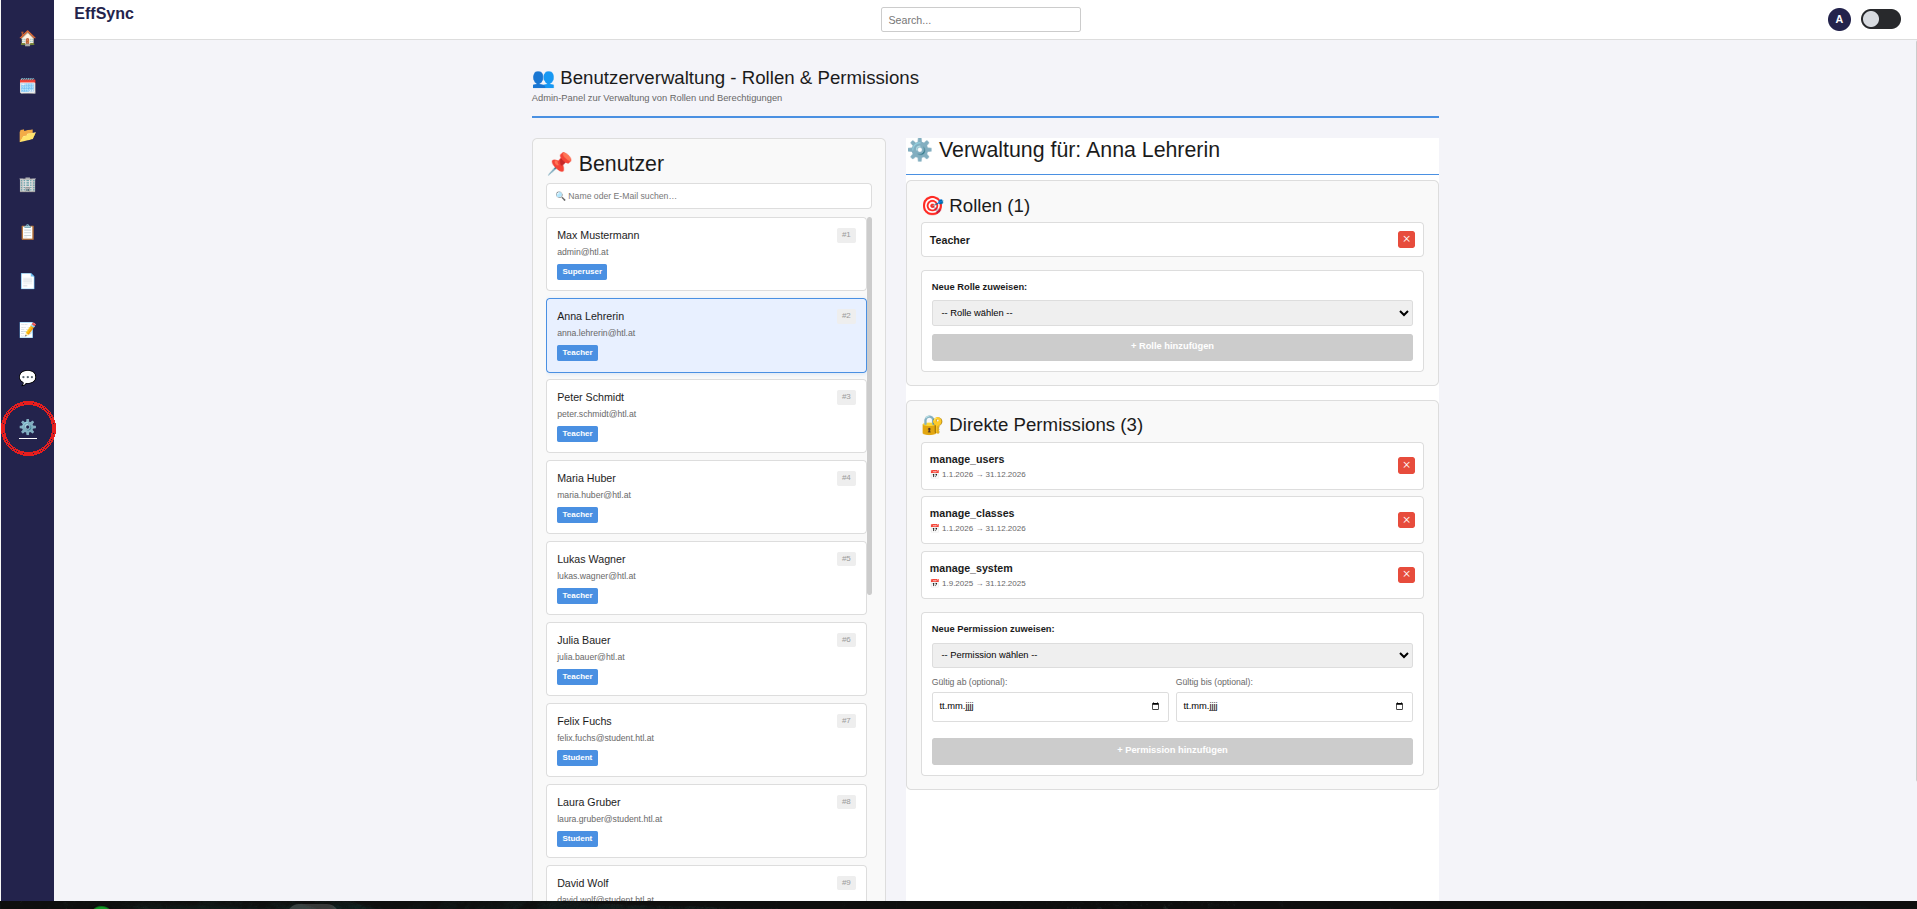
\includegraphics[width=0.95\textwidth]{content/bilder/admin_rollen_permissions.png}
  \caption{Admin-Oberfläche zur Verwaltung von Rollen und Berechtigungen; die rote Markierung zeigt das Zahnrad-Icon in der Seitenleiste, über das der Bereich erreichbar ist}
  \label{fig:admin_rollen_permissions}
\end{figure}

\authorsection{Kommunikation}{Ereny Micail}
\label{sec:kommunikation}
Die Kommunikation wird in \textit{EffSync} als integraler Bestandteil der Projektarbeit umgesetzt. Anstatt auf externe Messenger auszuweichen, erfolgt der Austausch direkt innerhalb der Plattform. Dadurch bleiben Nachrichten im fachlichen Kontext der jeweiligen Aufgaben bzw. Projekträume und sind für alle berechtigten Beteiligten nachvollziehbar.

Für die technische Umsetzung wird auf WebSockets gesetzt, da klassische REST-Schnittstellen keine bidirektionale Echtzeitkommunikation ermöglichen. Das Backend verteilt neue Nachrichten serverseitig per Push-Mechanismus an alle verbundenen Clients eines Raums. Dadurch erscheinen neue Inhalte ohne manuelles Aktualisieren der Benutzeroberfläche.

\authorsection{Benachrichtigungen}{Ereny Micail}
\label{sec:benachrichtigungen}
Benachrichtigungen dienen dazu, relevante Ereignisse unmittelbar sichtbar zu machen, etwa neue Nachrichten, Statusänderungen oder mitgliedschaftsrelevante Aktionen. Die Übertragung erfolgt ereignisgesteuert über die bestehende Echtzeitinfrastruktur. Dadurch reduziert sich die Reaktionszeit der Benutzer deutlich, und kritische Änderungen gehen im Arbeitsfluss nicht verloren.

Aus architektonischer Sicht folgt die Benachrichtigungslogik dem Prinzip, nur fachlich relevante Events zu publizieren. Damit wird unnötige Client-Last vermieden und die Oberfläche bleibt trotz häufiger Ereignisse übersichtlich.

\authorsection{Kalender}{Ereny Micail}
\label{sec:kalender}
Die Kalenderfunktion ergänzt die Aufgabenverwaltung um eine zeitliche Perspektive. Deadlines aus Tasks können in einer kalenderartigen Sicht zusammengeführt werden, wodurch zeitliche Abhängigkeiten und Belastungsspitzen früh erkennbar sind. Dies unterstützt sowohl die individuelle Lernorganisation als auch die Koordination in Teams.

In Verbindung mit Prioritäten und Statusinformationen entsteht eine konsistente Planungsgrundlage: Benutzer sehen nicht nur \textit{was} zu erledigen ist, sondern auch \textit{bis wann} und in welcher Dringlichkeit. Dadurch verbessert die Kalenderintegration die praktische Umsetzbarkeit der zuvor definierten Task-Strukturen.


\authorsection{Taskverwaltung}{Dražen Plavšić}
\label{sec:taskverwaltung}
Da \textit{EffSync} als Task-Management-System konzipiert ist, bildet das Task-Modul das zentrale Element der Anwendung. Die Zielsetzung des Systems ist es, sowohl Schülern als auch Lehrern die Verwaltung von Aufgaben zu erleichtern. Schüler erhalten die Möglichkeit, ihre Aufgaben eigenständig zu organisieren, während Lehrern ein strukturiertes Werkzeug zur Verfügung steht, um Aufgaben gezielt zuzuweisen und deren Bearbeitung zu überwachen.

Das System wurde dabei bewusst über den schulischen Kontext hinaus konzipiert. Durch die Möglichkeit der beliebig tiefen Verschachtelung von Tasks und Subtasks lassen sich nicht nur einfache Aufgaben, sondern auch komplexe Projektstrukturen abbilden. Ein einzelner Task kann dabei ein übergeordnetes Projekt repräsentieren, dessen Teilaufgaben in weitere Unteraufgaben unterteilt werden. Dies macht das Task-Modul von \textit{EffSync} grundsätzlich auch für den unternehmensinternen Einsatz geeignet, da sich ganze Projekte oder Teilprojekte vollständig innerhalb des Systems strukturieren lassen.

\subsection{Datenbankschema und grundlegender Aufbau eines Tasks}{Dražen Plavšić}
Bevor komplexe Mechanismen wie Taskhierarchien und automatische Evaluierungsregeln betrachtet werden, ist es wichtig den grundlegenden strukturellen Aufbau eines \textit{Tasks} zu verstehen. Die Task-Entität bildet das zentrale Kernstück der Applikation und ist in der Datenbank so modelliert, dass sie alle Metadaten für das Projektmanagement effizient speichern kann.

\begin{figure}[H]
  \centering
  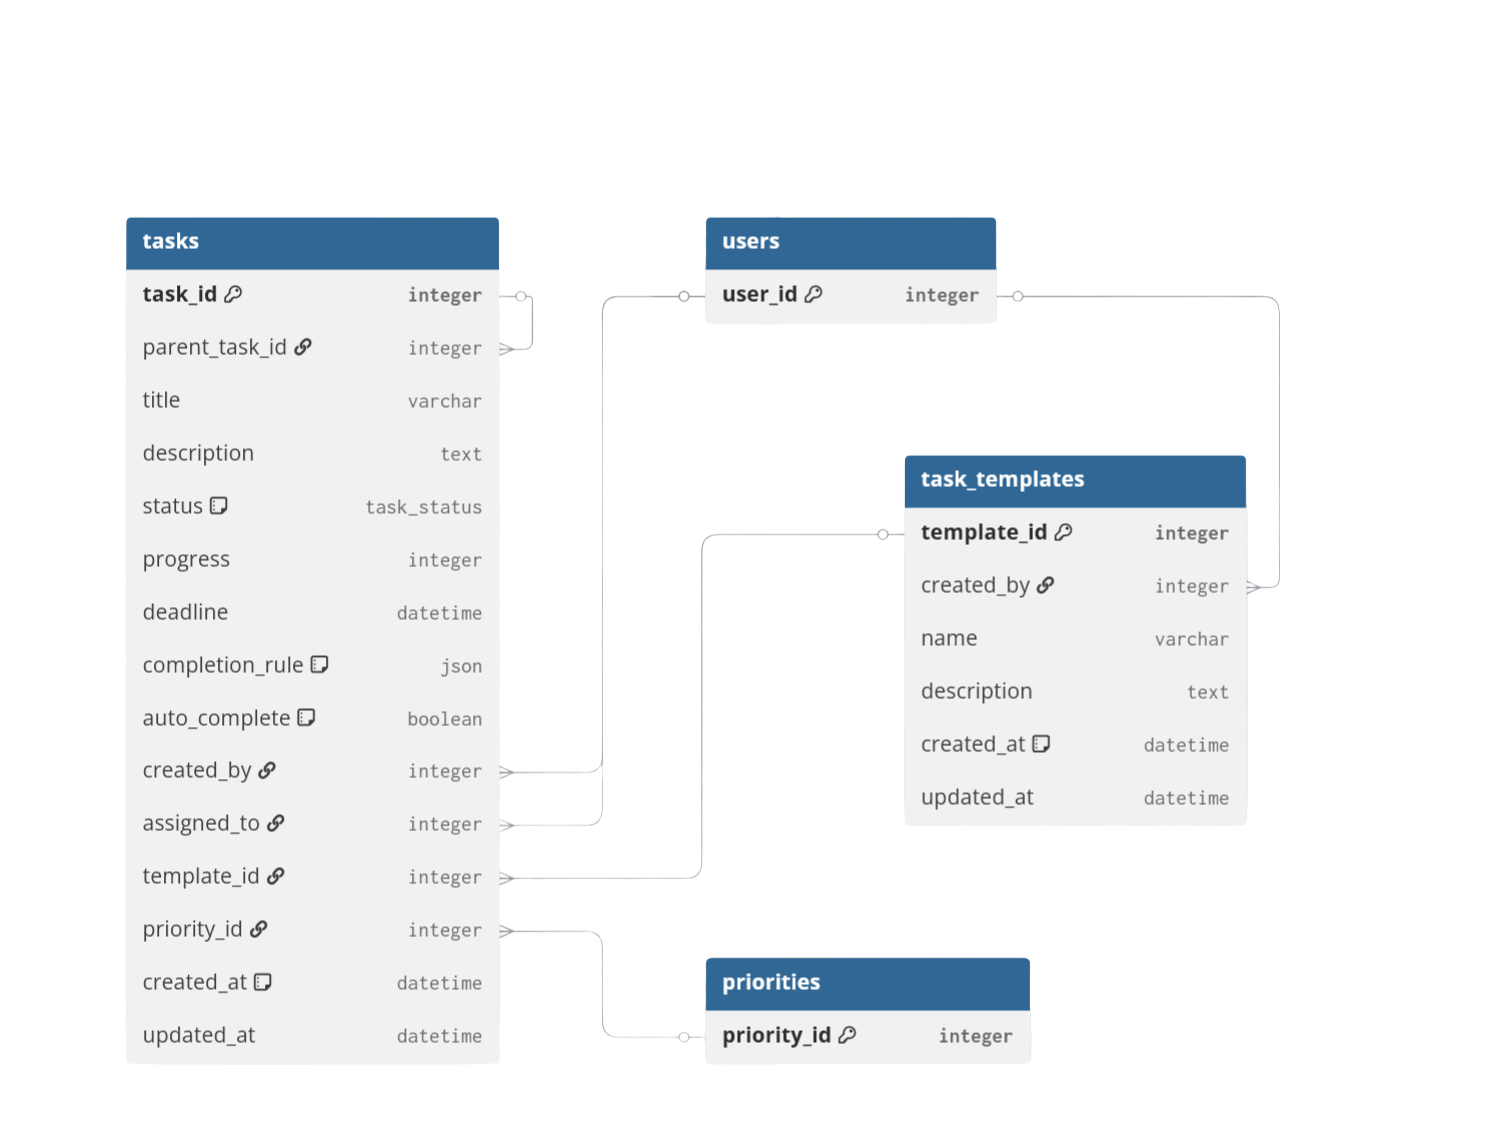
\includegraphics[width=0.8\textwidth]{content/bilder/task_db_schema.png}
  \caption{Auszug des Datenbankschemas zur Verwaltung der Tasks}
  \label{fig:task_schema}
\end{figure}

Die Tasks-Tabelle (siehe Abbildung \ref{fig:task_schema}) lässt sich logisch in drei wesentliche Datenbereiche unterteilen:
\begin{itemize}
    \item \textbf{Basisdaten \& Fortschritt:} Felder wie \texttt{title}, \texttt{description}, \texttt{status} und \texttt{progress} bilden die Kerninformationen für die Benutzeroberfläche. Der Status und der Fortschritt (0 bis 100\,\%) sind logisch aneinander gekoppelt.
    \item \textbf{Verantwortlichkeiten \& Organisation:} Über \texttt{created\_by} und \texttt{assigned\_to} wird auf Datenbankebene sichergestellt, dass jede Aufgabe einem Ersteller und optional einem Bearbeiter zugewiesen ist. Das Feld \texttt{priority\_id} referenziert eine separate Tabelle, um Tasks nach Dringlichkeit (z.\,B. niedrig, hoch) zu kategorisieren, während \texttt{deadline} die zeitliche Frist setzt.
    \item \textbf{Architektonische Steuerungsfelder:} Die Spalte \texttt{parent\_task\_id} dient als Selbstreferenz (\textit{Self-Join}) auf die gleiche Tabelle, um unendlich tiefe Task-Bäume zu ermöglichen. Die Felder \texttt{completion\_rule} (vom Datentyp JSONB) und \texttt{auto\_complete} sind speziell für die eigens entwickelte Rule-Engine reserviert.
\end{itemize}

Dieser Aufbau bildet das Fundament für die gesamte Geschäftslogik der Taskverwaltung, die in den folgenden Abschnitten detailliert erläutert wird.

\subsection{Hierarchie der Tasks}{Dražen Plavšić}
Jeder Task kann über das Feld \texttt{parent\_task\_id} einem übergeordneten Task zugewiesen werden. Dadurch entsteht eine hierarchische Baumstruktur (\textit{Tree Structure})\cite{celko2004trees}, bei der ein Haupt-Task theoretisch unendlich viele Subtasks und deren Nachkommen (\textit{Descendants}) besitzen kann.

Diese strukturelle Flexibilität bringt jedoch eine technische Herausforderung mit sich: die Vermeidung von \textit{Circular References}. Wenn Task A der übergeordnete Task von Task B ist, darf Task B nicht nachträglich als übergeordneter Task von Task A definiert werden. Ebenso darf ein Task nicht sein eigener Parent werden, da dies unweigerlich zu Endlosschleifen beim Auslesen der Daten führen würde.

Um die Datenintegrität aufrechtzuerhalten, implementiert das Backend bei jeder Zuweisung oder Änderung eines Parent-Tasks eine Sicherheitsprüfung. Wie in Listing \ref{lst:circular_reference} dargestellt, traversiert die Methode \texttt{validateNoCircularReference} den Baum iterativ von unten nach oben. Dabei speichert sie alle bereits besuchten Task-IDs in einem \texttt{Set}. Sobald die Methode auf einen Task stößt, dessen ID bereits im Set existiert, greift der Schutzmechanismus und das System bricht den Vorgang mit einer \texttt{BadRequestException} (HTTP Status 400) ab.

\begin{listing}[H]
\begin{minted}{typescript}
// Backend: TasksService
private async validateNoCircularReference(taskId: number, parentTaskId: number): Promise<void> {
  let currentTask = await this.prisma.tasks.findUnique({
    where: { task_id: parentTaskId },
    select: { task_id: true, parent_task_id: true },
  });
  // Set initialisieren, um bereits besuchte Knoten zu speichern
  const visited = new Set<number>([taskId]);
  while (currentTask) {
    if (visited.has(currentTask.task_id)) {
      throw new BadRequestException(
        'Circular reference detected: Task cannot be ancestor of itself'
      );
    }
    visited.add(currentTask.task_id);
    if (!currentTask.parent_task_id) break;
    // Nächsten Knoten in der Hierarchie abfragen
    currentTask = await this.prisma.tasks.findUnique({
      where: { task_id: currentTask.parent_task_id },
      select: { task_id: true, parent_task_id: true },
    });
  }
}
\end{minted}
\caption{Schutz vor Zirkelbezügen durch Traversierung der Baumstruktur}
\label{lst:circular_reference}
\end{listing}

Beim Abrufen der hierarchischen Daten aus der Datenbank nutzt das Backend zwei optimierte Strategien, um verschachtelte Strukturen effizient an das Vue.js-Frontend zu liefern. Für den allgemeinen Listenaufruf sammelt die Hilfsfunktion \texttt{collectDescendants} alle Nachkommen eines Tasks rekursiv über mehrere Datenbankabfragen ein und führt die Ergebnisse im Speicher zusammen. Für die vollständige Baumansicht hingegen werden mit der Methode \texttt{findeOneWithSubtasks} alle relevanten Tasks in \textbf{einer einzigen} Datenbankabfrage geladen und an die \texttt{buildTree} Methode übergeben, welche das Ergebnis serverseitig als tief verschachteltes JSON-Objekt rekonstruiert (siehe Listing \ref{lst:build_tree}).

\begin{listing}[H]
\begin{minted}{typescript}
// Backend: TasksService
async findeOneWithSubtasks(taskId: number, includeRelations = true) {
const rootTask = await this.prisma.tasks.findUnique({
where: { task_id: taskId },
});
// Alle Tasks des Erstellers in einer einzigen Abfrage laden
const allTasks = await this.prisma.tasks.findMany({
where: { created_by: rootTask.created_by },
include: includeRelations ? this.basicInclude() : undefined,
});
// Serverseitige Rekonstruktion als verschachtelter JSON-Baum
return this.buildTree(allTasks, taskId);
}
private buildTree(allTasks: any[], taskId: number) {
const taskMap = new Map();
allTasks.forEach(task =>
taskMap.set(task.task_id, { ...task, subtasks: [] })
);
taskMap.forEach(task => {
const parentTaskId = taskMap.get(task.parent_task_id);
parentTaskId?.subtasks.push(taskMap.get(task.task_id));
});
return taskMap.get(taskId); // Gibt das vollständige JSON-Objekt zurück
}
\end{minted}
\caption{Serverseitige Rekonstruktion des Task-Baums als verschachteltes JSON-Objekt}
\label{lst:build_tree}
\end{listing}

Dieses verschachtelte JSON-Objekt wird anschließend über die \gls{REST-API} direkt an das Vue.js-Frontend übertragen, welches die Struktur ohne weitere Transformationen für die Darstellung der Baumansicht verwenden kann.

\subsection{Rule-Engine und automatische Task-Validierung}{Dražen Plavšić}
\textit{EffSync} besitzt auch die Fähigkeit, übergeordnete Tasks automatisch abzuschließen (\textit{Auto-Completion}), sobald bestimmte vom Nutzer definierte Kriterien der zugehörigen Subtasks erfüllt sind. Um dies zu realisieren, wird eine eigene \textit{Rule-Engine} implementiert, die in einen visuellen Frontend-Builder und einen serverseitigen Evaluator unterteilt ist.

Im Vue.js-Frontend ermöglicht die Komponente \texttt{RuleBuilder} dem Ersteller eines Tasks, logische Bedingungen zu definieren. Dabei können einzelne Subtasks beliebig tief mit logischen Operatoren (\texttt{UND}, \texttt{ODER}, \texttt{XOR}, \texttt{NICHT}) verknüpft werden. Das Frontend übersetzt diese visuelle Darstellung in einen 
\gls{AST} im JSON-Format und übermittelt diesen an das Backend, wo er als \texttt{JSONB}\cite{postgresql_jsonb} abgespeichert wird.

Sobald der Status eines Subtasks geändert wird (beispielsweise auf \texttt{COMPLETED}), löst das Backend einen Event-Trigger aus. Die serverseitige Engine lädt daraufhin den JSONB-Regelbaum des übergeordneten Tasks und wertet diesen aus. Da der Baum beliebig tief verschachtelt sein kann, erfolgt die Auswertung über einen rekursiven Algorithmus.

Wie in Listing~\ref{lst:rule_evaluator} gezeigt, traversiert die Funktion \texttt{evaluateCondition} den JSON-Baum. Handelt es sich bei dem aktuellen Knoten (\textit{Node}) um ein Endblatt (\textit{Leaf}), wird geprüft, ob der referenzierte Task abgeschlossen ist. Handelt es sich hingegen um einen Operator, ruft sich die Funktion für alle angehängten Bedingungen (\textit{Operands}) selbst auf und verknüpft die booleschen Ergebnisse anschließend anhand des jeweiligen logischen Operators.

\begin{listing}[H]
\begin{minted}{typescript}
// Backend: task.evaluator.completion.ts
export function evaluateCondition(
    node: ConditionNode,
    completedTaskIds: Set<string>,
): boolean {
    // Abbruchbedingung der Rekursion: Blattknoten (konkreter Task)
    if (node.type === 'leaf') {
        return completedTaskIds.has(String(node.task_id));
    }
    // Rekursiver Aufruf für alle Kind-Knoten
    const results = node.operands.map(operand =>
        evaluateCondition(operand, completedTaskIds),
    );
    // Auswertung anhand des logischen Operators
    switch (node.operator) {
        case 'AND': return results.every(r => r === true);
        case 'OR':  return results.some(r => r === true);
        case 'XOR': return results.filter(r => r === true).length === 1;
        case 'NOT': return !results[0];
    }
}
\end{minted}
\caption{Rekursive Auswertung des JSONB-Baums zur Task-Validierung}
\label{lst:rule_evaluator}
\end{listing}

Ergibt die Evaluierung des gesamten Baums den Wert \texttt{true}, setzt die Engine den Status des Parent-Tasks automatisch auf \texttt{COMPLETED}. Gleichzeitig wird über das WebSocket-Gateway ein Echtzeit-Event an das Frontend gesendet, um die Benutzeroberfläche aller beteiligten Nutzer ohne Verzögerung zu aktualisieren.

\subsection{Benutzerinteraktion, Usability und Sicherheit}
Neben einer performanten Datenverarbeitung im Hintergrund liegt ein wesentlicher Fokus der Taskverwaltung auf der Benutzerfreundlichkeit (\textit{Usability}) und dem Schutz vor Bedienfehlern im Vue.js-Frontend. 

Um dem Nutzer die Verwaltung einer Vielzahl von Aufgaben zu erleichtern, wird eine dynamische Filter- und Suchfunktion (\texttt{useTaskFilters}) implementiert. Diese ermöglicht es, die Aufgabenliste auf Seiten der Clients, also ohne erneute Datenbankabfrage, in Echtzeit nach Status, Priorität oder Freitext zu filtern und zu sortieren. Die Priorisierung der Aufgaben ist dabei in vier Stufen unterteilt (niedrig, mittel, hoch, dringend), was eine effiziente Arbeitsorganisation unterstützt.

Besonderes Augenmerk wird auf die Datenintegrität und die Vermeidung von ungewolltem Datenverlust gelegt. Das Löschen von Tasks ist daher mit mehrstufigen Sicherheitsmechanismen versehen. Versucht ein Nutzer einen Task zu löschen, der noch aktive Subtasks enthält, lehnt das Backend die Anfrage direkt ab. Dieses Verhalten entspricht dem Prinzip der referentiellen Integrität, bei dem abhängige Kindeinträge das Löschen eines Elterndatensatzes verhindern\cite{postgresql_constraints}. Das System verlangt in diesem Fall zwingend, dass die untergeordneten Aufgaben (\textit{Dependencies}) zuerst gelöscht oder einem anderen Parent-Task zugewiesen werden.

Um zudem versehentliche Löschungen von wichtigen Hauptaufgaben durch simple Fehleingaben (z.\,B.\ durch einen unachtsamen Klick) zu verhindern\cite{uxpsychology_destructive}\cite{nielsen_heuristics}, wurde eine zusätzliche Hürde im Frontend etabliert.

\begin{figure}[H]
  \centering
  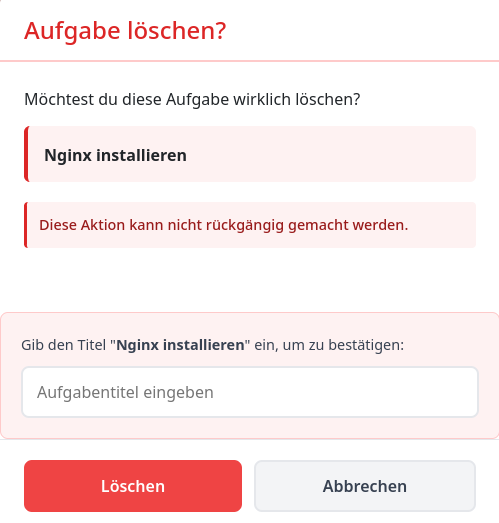
\includegraphics[width=0.4\textwidth]{content/bilder/task_delete_dilog.png}
  \caption{Bestätigungsfenster beim Löschen eines Tasks}
  \label{fig:task_delete}
\end{figure}

Wie Abbildung \ref{fig:task_delete} zeigt, muss der Nutzer bei kritischen Löschvorgängen den exakten Namen des Tasks in ein Dialogfenster abtippen. Erst wenn die Eingabe zeichengenau mit dem Task-Titel übereinstimmt, wird der Lösch-Button freigeschaltet.

Darüber hinaus existieren strikte Prüfungen beim Ändern des Task-Status. Ein Task kann nicht in den Status \texttt{COMPLETED} (Erledigt) übergehen, wenn der verknüpfte Arbeitsfortschritt (\textit{Progress}) noch nicht bei 100\,\% liegt. Auch hier arbeiten Frontend und Backend Hand in Hand: Das UI blockiert die Checkbox visuell, während das Backend bei einem API-Aufruf die Validierung der Werte erzwingt, um inkonsistente Zustände in der Datenbank zu verhindern.

\subsection{Task-Templates zur Effizienzsteigerung}
Da sich viele Arbeitsabläufe, wie beispielsweise Assignments aus Schulfächern (z.\,B.\ POS oder DB), Hausaufgaben für Schüler oder klassische Arbeitspakete in einem Softwareprojekt (z.\,B.\ das Implementieren von Unit-Tests), in ihrer Form und Struktur ähneln und regelmäßig wiederholen, ermöglicht \textit{EffSync} das Abspeichern von Tasks als Vorlage (\textit{Template}). 

Die Verwendung von Vorlagen zur Wiederverwendung wiederkehrender Aufgabenstrukturen ist eine etablierte Praxis in modernen Projektmanagement-Werkzeugen \cite{nielsen_heuristics} und reduziert gemäß dem UX-Prinzip der Effizienz redundante Dateneingaben für erfahrene Nutzer.

Möchte der Nutzer nun einen neuen Arbeitsauftrag erstellen, kann er direkt auf ein gespeichertes Template zurückgreifen. Das Frontend lädt die entsprechenden Parameter aus dem Backend und füllt die Eingabemasken der Benutzeroberfläche automatisch aus. Der Nutzer muss anschließend lediglich aufgabenspezifische, variable Details, wie etwa eine neue Deadline oder eine abweichende Zuweisung (\texttt{assigned\_to}), anpassen, bevor der finale Task generiert wird.

\authorsection{Notizverwaltung}{Ereny Micail}
\label{sec:notizverwaltung}
Die Notizverwaltung erweitert das Task-Modul um eine bewusst einfache Möglichkeit, Informationen schnell und ohne feste Struktur abzulegen. Während Tasks in \textit{EffSync} auf planbare Arbeitseinheiten mit Status, Priorität, Fälligkeit und Zuständigkeiten ausgelegt sind, dienen Notizen als flexibler Zwischenspeicher für Inhalte, die (noch) nicht in ein konkretes Aufgabenmodell passen.

Technisch ist die Notizfunktion als eigenständige Entität umgesetzt, um die strukturierte Aufgabenplanung klar von der freien Textdokumentation zu trennen. Eine Notiz umfasst einen \texttt{title} und eine \texttt{description} und ist eindeutig einem Benutzer zugeordnet. So lassen sich Gedanken, Besprechungsergebnisse, Lehrinhalte oder spontane Ideen ohne zusätzlichen Verwaltungsaufwand erfassen.

Die Geschäftslogik folgt dem bekannten \textit{Create, Read, Update, Delete} (CRUD)-Muster: Nutzer können Notizen anlegen, einsehen, bearbeiten, auflisten und löschen. Anders als bei Tasks wird bewusst auf komplexe Funktionen wie Hierarchien, Fortschrittsmodelle oder automatische Auswertungsregeln verzichtet. Diese Reduktion senkt den Bedienaufwand im Interface und erleichtert die schnelle Erfassung im Arbeitsalltag.

Im Frontend führt dies zu einer schlanken Interaktion: Nach dem Anlegen steht der Notizinhalt sofort bereit und kann bei Bedarf kontinuierlich angepasst werden. Die Notizverwaltung wirkt damit als leichtgewichtiges Pendant zur Taskverwaltung und schließt die Lücke zwischen formaler Aufgabenplanung und informeller Wissenssammlung.

Architektonisch stärkt das Modul die Trennung von Verantwortlichkeiten (\textit{Separation of Concerns}): Tasks bleiben prozessorientiert und auswertbar, Notizen fungieren als freiformorientierter Informationsspeicher. Dadurch steigt die Praxistauglichkeit von \textit{EffSync}, weil Informationen nicht zwanghaft in die starre Struktur eines Tasks gepresst werden müssen.

\authorsection{Live-Chat}{Dražen Plavšić}
\label{sec:live_chat}

Im akademischen Umfeld der HTL, aber auch in der modernen Softwareindustrie zeigt sich bei der Projektarbeit häufig ein wiederkehrendes Problem: Etablierte Task-Management-Lösungen bieten meist keine native, integrierte Echtzeitkommunikation\cite{trello_powerup_boardchat}\cite{atlassian_jira_11_3_documentation}\cite{atlassian_trello_guide}\cite{atlassian_trello_tour}. Dies zwingt Arbeitsgruppen dazu für Absprachen auf externe Kommunikationsplattformen wie Discord, Slack, WhatsApp oder Microsoft Teams auszuweichen. Dieser ständige Plattformwechsel (\textit{Context Switching}) führt zu einem fragmentierten Informationsfluss, bei dem Projektkontext und Aufgabenbezug schnell verloren gehen. 

Um dieses Problem zu lösen, wird in \textit{EffSync} ein nativer Live-Chat implementiert. Diese nahtlose Verschmelzung von Aufgabenverwaltung und Echtzeitkommunikation stellt die \textit{Unique Selling Proposition} (USP) der Applikation dar. 

\subsection{Technologische Umsetzung mittels WebSockets}
Da klassische REST-Schnittstellen auf dem Request-Response-Prinzip basieren, eignen sie sich nicht für Echtzeitanwendungen, da sie keine serverseitige Push-Kommunikation unterstützen~\cite{websocket_restapi_hybrid}. Ein ständiges Abfragen des Servers (\textit{HTTP-Polling}) nach neuen Nachrichten würde zudem unnötige Netzwerklast erzeugen, da jede HTTP-Anfrage einen erheblichen Protokoll-Overhead mit sich bringt~\cite{diva_polling_ws_2017}. Daher wird die Chat-Funktion vollständig über \textit{WebSockets} realisiert. Im Backend kommen hierbei NestJS-Gateways zum Einsatz, welche eine dauerhafte, bidirektionale Verbindung zum Vue-Frontend aufrechterhalten. Sendet ein Nutzer eine Nachricht, wird diese vom Server validiert und in Echtzeit per Push-Verfahren an alle relevanten Clients im jeweiligen Chatraum (\textit{Room}) verteilt (siehe Abbildung \ref{fig:datenfluss_websocket}).
\begin{figure}[H]
  \centering
  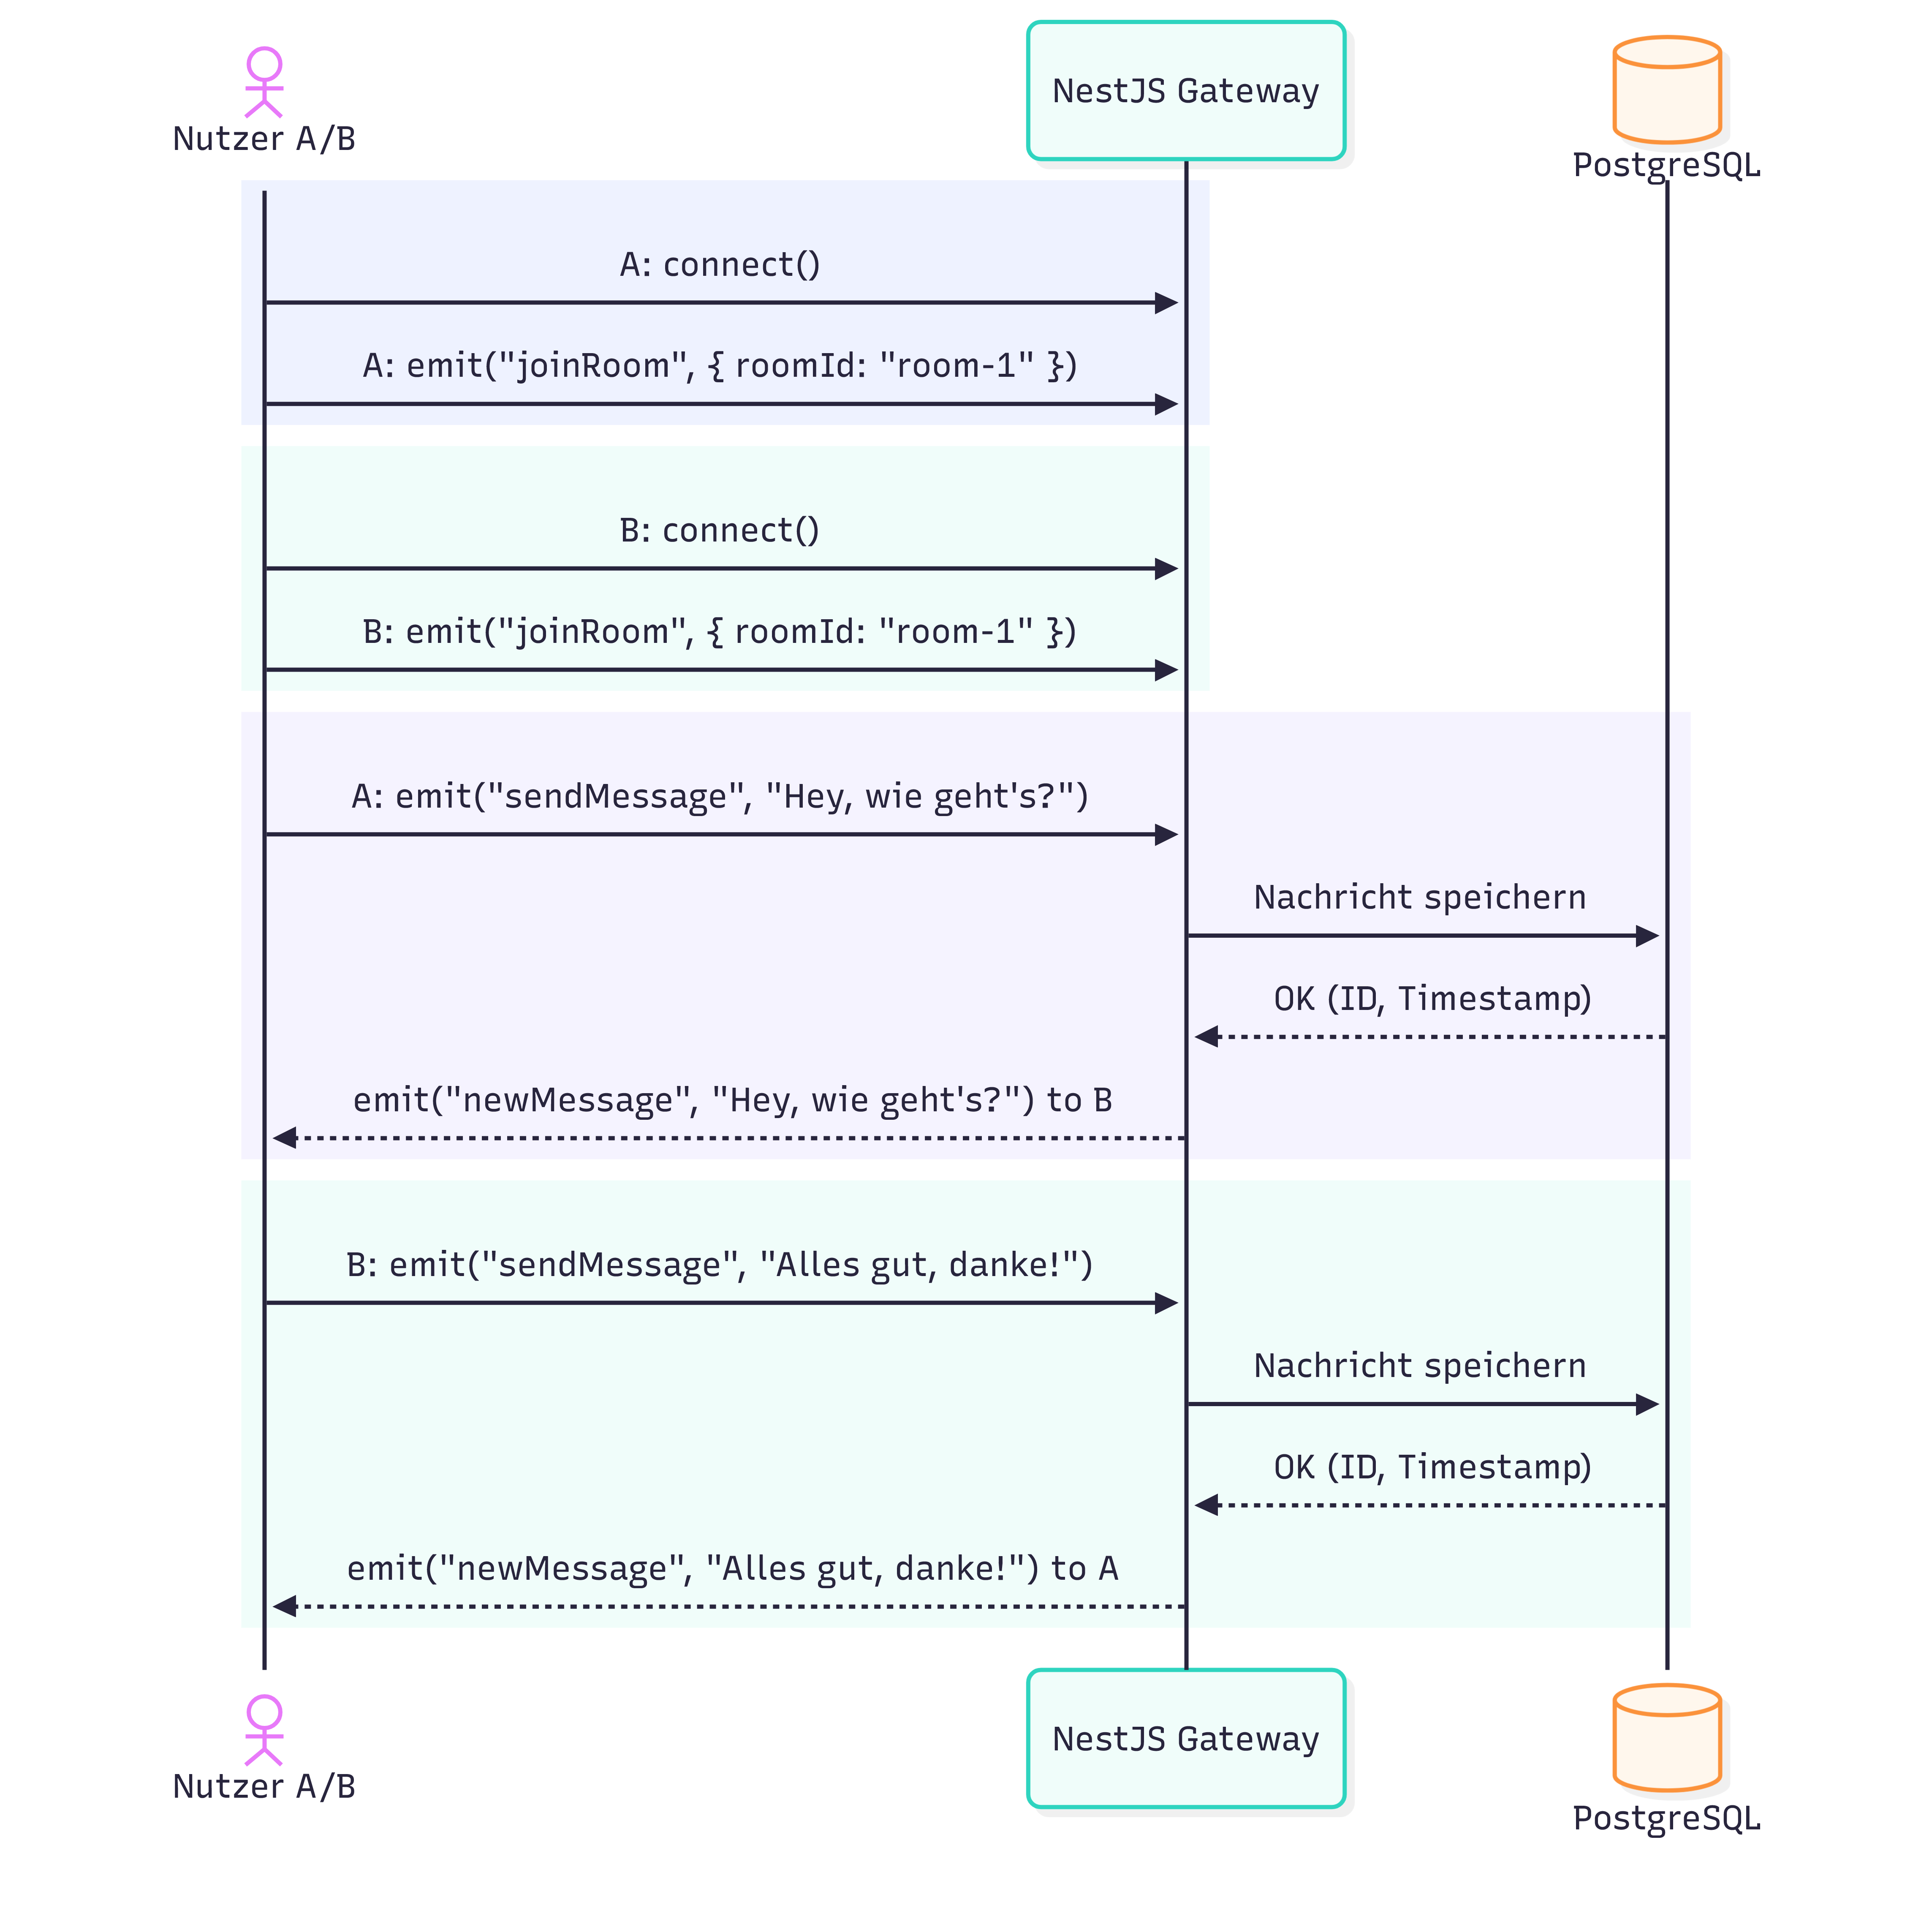
\includegraphics[width=0.6\textwidth]{content/bilder/realtime_chat_simpler_no_notes.png}
  \caption{Echtzeit-Datenfluss via WebSockets}
  \label{fig:datenfluss_websocket}
\end{figure}

\subsection{Unterscheidung der Chat-Typen und Vermeidung von Duplikaten}
In \textit{EffSync} wird das Chat-System prinzipiell in zwei Raumtypen (\textit{Rooms}) unterteilt: private 1-zu-1-Chats und projektbezogene Gruppenchats. Diese Unterscheidung ist nicht nur für die Darstellung in der Benutzeroberfläche relevant, sondern vor allem für die Datenmodellierung und die Berechtigungslogik wichtig. 

Wie im Datenbankschema (siehe Abbildung \ref{fig:chat_schema}) zu erkennen ist, wird der Raumtyp über das Flag \texttt{is\_private} in der Tabelle \texttt{chat\_rooms} gesteuert. Bei Gruppenchats kann zudem optional eine direkte Verknüpfung zur entsprechenden Aufgabe (\texttt{task\_id}) hergestellt werden.

\begin{figure}[H]
    \centering
    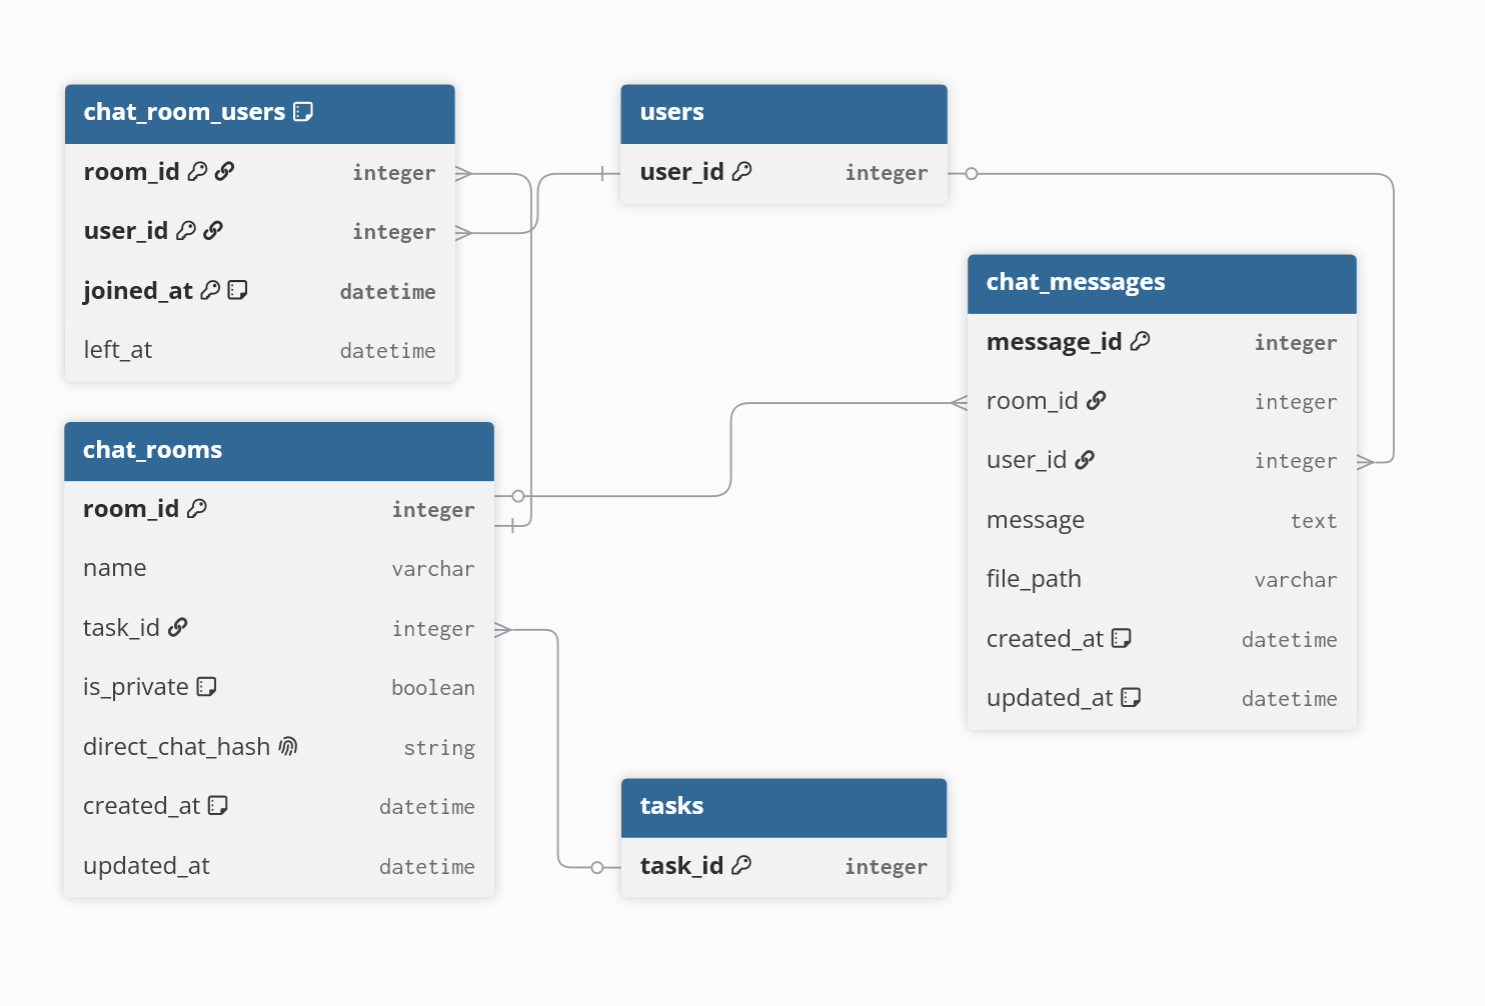
\includegraphics[width=0.8\textwidth]{content/bilder/chat_db_schema.png}
    \caption{Auszug des Datenbankschemas zur Verwaltung der Chaträume}
    \label{fig:chat_schema}
\end{figure}

Bei der Initialisierung von privaten Chats greift serverseitig eine spezielle Validierungslogik, um die Erstellung redundanter Chaträume zu verhindern. Möchte Nutzer A einen Chat mit Nutzer B starten, muss sichergestellt werden, dass für diese Konstellation nicht bereits ein Raum existiert. Anstatt hierfür eine rechenintensive Datenbankabfrage über die Mitgliedertabelle durchzuführen, wird dies über das Feld \texttt{direct\_chat\_hash} in der Tabelle \texttt{chat\_rooms} (siehe Abbildung \ref{fig:chat_schema}) gelöst. 

Aus den Identifikationsnummern der beiden Teilnehmer wird ein deterministischer String generiert (beispielsweise \texttt{user1\_user2}). Da dieses Feld in der Datenbank mit einem \texttt{UNIQUE}-Constraint versehen ist, wird die Erstellung eines Duplikats bereits auf Datenbankebene strikt abgelehnt. Schlägt der Erstellungsversuch aufgrund des Constraints fehl, wird die Erstellung blockiert und dem Client stattdessen die ID des bestehenden Raums zurückgegeben. Dies garantiert, dass die Konversation zwischen zwei Personen nicht fragmentiert wird, sondern die gesamte Historie stets in einem einzigen, fortlaufenden Chatverlauf bleibt.

\subsection{Raumverwaltung und Berechtigungslogik}
Während in einem privaten Chat beide Teilnehmer gleichgestellte Rechte besitzen, erfordern Gruppenchats eine hierarchische Rollenverteilung, um administrative Aufgaben abzubilden. Die Komplexität liegt hierbei in der sicheren Verwaltung der Zugriffsrechte (\textit{Authorization}). Ein exemplarisches Sicherheitsszenario ist das Entfernen von Mitgliedern aus einem Gruppenchat. 

Wie in Listing~\ref{lst:chat_permissions} dargestellt, wurde im Backend eine strikte Berechtigungslogik implementiert, die bei Modifikationen der Raummitglieder zwischen zwei Szenarien unterscheidet: Möchte ein Nutzer den Chatraum freiwillig verlassen (\texttt{requesterId === targetUserId}), wird die Aktion ohne weitere Prüfung gestattet. Versucht jedoch ein Nutzer eine andere Person aus dem Gruppenraum zu entfernen, greift eine Sicherheitsprüfung (\texttt{assertIsCreator}). Diese stellt sicher, dass ausschließlich der ursprüngliche Ersteller des Chatraums das Recht besitzt, andere Mitglieder auszuschließen. Andernfalls meldet das System aus Sicherheitsgründen sofort eine \texttt{ForbiddenException} (HTTP Status 403).

\begin{listing}[H]
\begin{minted}{typescript}
// Backend: ChatRoomsService
async removeMember(roomId: number, requesterId: number, targetUserId: number) {
    // Szenario B: User versucht jemand anderen zu entfernen
    if (requesterId !== targetUserId) {
        // Prüft, ob der Requester der Creator des Gruppenraums ist. 
        // Wirft intern eine ForbiddenException, falls nicht.
        await this.chatRoomsService.assertIsCreator(roomId, requesterId);
    }
    // Szenario A (User entfernt sich selbst) oder
    // Szenario B (Creator entfernt User) war erfolgreich:
    return this.chatRoomMembersRepository.delete({ roomId, userId: targetUserId });
}
async assertIsCreator(roomId: number, userId: number) {
    // Raum anhand der roomId aus der Datenbank laden,
    // nur das Feld created_by wird benötigt.
    const room = await this.prisma.chat_rooms.findUnique({
        where: { room_id: roomId },
        select: { created_by: true },
    });
    // Raum existiert nicht → 404
    if (!room) throw new NotFoundException('Room not found!');
    // Prüft, ob der anfragende User der Ersteller des Raums ist.
    // Falls nicht → 403 ForbiddenException
    if (room.created_by !== userId)
        throw new ForbiddenException('Only the room creator can do this!');
}
\end{minted}
\caption{Berechtigungsprüfung beim Entfernen von Mitgliedern aus einem Gruppenchat}
\label{lst:chat_permissions}
\end{listing}
    \authorchapter{Testing und Qualitätssicherung}{Ereny Micail}
\label{ch:testing_quality}
Die Qualitätssicherung ist ein wesentlicher Bestandteil des Softwareentwicklungsprozesses. Um sicherzustellen, dass \textit{EffSync} funktional korrekt, stabil und wartbar umgesetzt wird, wurde ein mehrstufiges Testkonzept definiert.

Dieses Kapitel beschreibt die eingesetzten Verfahren zur systematischen Prüfung des Systems. Zunächst wird die Teststrategie als methodischer Rahmen vorgestellt. Anschließend werden die implementierten Testarten von isolierten Unit-Tests über API-Tests bis hin zu E2E-Tests erläutert.

Ergänzend werden die Usability-Tests zur Bewertung der Bedienbarkeit sowie die Fehleranalyse zur Dokumentation und Nachverfolgung identifizierter Probleme dargestellt.

\authorsection{Teststrategie}{Dražen Plavšić}
\label{sec:test_strategie}

Um die Stabilität und Wartbarkeit von \text{EffSync} zu gewährleisten, wird für dieses Projekt eine mehrstufige Teststrategie definiert. Diese orientiert sich konzeptionell an der klassischen Testpyramide nach Mike Cohn \cite{cohn2009succeeding} (siehe Abbildung \ref{fig:testpyramide}). 

\begin{figure}[H]
    \centering
    \includesvg[width=0.4\textwidth]{content/bilder/test_pyramide.svg} 
    \caption{Die Testpyramide für das \textit{EffSync}-Projekt in Anlehnung an Mike Cohn}
    \label{fig:testpyramide}
\end{figure}

Wie in Abbildung \ref{fig:testpyramide} zu sehen ist, bilden die Unit-Tests das Fundament der Pyramide, welche die größte Menge an Tests ausmachen. Hierbei gilt das Grundprinzip: Je weiter unten in der Testpyramide eine Testebene angesiedelt ist, desto isolierter und schneller in der Ausführung sind die entsprechenden Tests. Auf der mittleren Ebene befinden sich die Integrations- und API-Tests, welche die Kommunikation zwischen den Schichten prüfen. Die Spitze der Pyramide bilden ausgewählte End-to-End-Tests (E2E), die isoliert kritische User-Flows aus der Perspektive des Endanwenders validieren.

\subsubsection{Richtlinien zur Testabdeckung (Code Coverage)}
In der Softwareentwicklung existiert kein universell gültiger oder verbindlich vorgeschriebener Prozentwert für die Testabdeckung. Selbst die internen Engineering-Richtlinien von Google \cite{google2020coverage} verzichten auf starre Vorgaben und empfehlen stattdessen zielgerichtete Werte, wobei 60\,\% als akzeptabel, 75\,\% als lobenswert und 90\,\% als vorbildlich eingestuft werden. 


Sicherheitskritische Bereiche, wie beispielsweise die Authentifizierungslogik oder Autorisierungs-Guards, streben eine Testabdeckung von über 90\,\% an, da ungetestete Code-Pfade in diesen Modulen ein erhebliches Sicherheitsrisiko darstellen. Für Standard-Controller oder Datentransferobjekte (DTOs) wurde hingegen kein fixer Prozentwert auf Unit-Ebene definiert, da deren Validierung systembedingt primär durch die höherstufigen API-Tests erfolgt. Bei den API- und E2E-Tests wird bewusst auf eine zeilenbasierte Code-Coverage verzichtet; stattdessen dient die Vollständigkeit der getesteten HTTP-Endpunkte und User-Flows als primäres Qualitätskriterium.

\authorsection{Unit-Tests}{Dražen Plavšić}
\label{sec:unit_tests}
Unit-Tests bilden das Fundament der Qualitätssicherung innerhalb von \textit{EffSync}. Ihr primärer Zweck besteht darin, einzelne funktionale Einheiten des Sourcecodes, wie Klassen, Methoden oder Komponenten, isoliert auf ihre korrekte Funktionsweise zu überprüfen. Da solche Einheiten in der Regel von weiteren Modulen oder externen Diensten abhängig sind, werden diese Abhängigkeiten in Unit-Tests gezielt simuliert. Dadurch lassen sich die Tests unter kontrollierten Bedingungen ausführen und das Verhalten der jeweiligen Einheit unabhängig bewerten.

\subsection{Testwerkzeuge und Zielvorgaben}
Für die technische Umsetzung werden zwei auf die jeweilige Umgebung abgestimmte Testwerkzeuge eingesetzt. Im \textbf{Backend (NestJS)} wird \textit{Jest} in Kombination mit \texttt{@nestjs/testing} verwendet\cite{nestjs_testing_docs}, im \textbf{Frontend (Vue 3)} \textit{Vitest}\cite{vitest_docs} zusammen mit \texttt{@vue/test-utils}\cite{vue_test_utils_docs}. Die Ausführung der Tests erfolgt über das Skript \texttt{npm run test:coverage}.

Anhand des zuvor definierten Ansatzes sind für die Unit-Tests spezifische Prioritäten und Abdeckungsziele (Code Coverage) für beide Systemkomponenten festgelegt:

\begin{itemize}
    \item \textbf{Kritische Priorität (Zielabdeckung $\ge$ 90\,\%):}\\
    Im Backend betrifft dies essenzielle Sicherheitskomponenten wie den \texttt{AuthService} (Token-Handling, Passwort-Hashing), Zugriffskontrollen (\texttt{JwtAuthGuard}, \texttt{LocalAuthGuard}) sowie die Kernlogik der Applikation (\texttt{TaskService}). Im Frontend liegt der Fokus auf der globalen Zustandsverwaltung, dem Pinia \texttt{Auth-Store} und \texttt{Task-Store}, sowie auf kritischen \textit{HTTP-Utility-Functions}.
    
    \item \textbf{Mittlere Priorität (Zielabdeckung $\ge$ 75\,\%):}\\
    Hierzu zählen im Backend weniger komplexe CRUD-Operationen (\texttt{UserService}) oder der \texttt{PermissionService}. Im Frontend fallen darunter unter anderem die \textit{Routen-Guards} des Vue Routers zur Verhinderung unberechtigter Weiterleitungen sowie wiederverwendbare komplexe UI-Komponenten.
    
    \item \textbf{Bereiche ohne spezifisches Abdeckungsziel:}\\
    Technischer Initialisierungscode (\texttt{main.ts}, \texttt{app.module.ts}), logikfreie Datenbank-Schemata (\textit{Prisma}) sowie reine CSS- und Layout-Komponenten sind von der Metrik ausgenommen, da ein isolierter Unit-Test an dieser Stelle keinen funktionalen Mehrwert bietet.
\end{itemize}

\subsection{Praktische Umsetzung und Mocking-Strategie}
Wie in Listing \ref{lst:unit_test_example} veranschaulicht, wird die Datenbankabhängigkeit vollständig durch das Test-Framework gemockt. Dadurch wird gewährleistet, dass ein Fehlschlagen des Tests ausschließlich auf einen Fehler in der Geschäftslogik des Services zurückzuführen ist und nicht durch externe Faktoren, wie eine fehlende Datenbankverbindung, verfälscht wird.

\begin{listing}[H]
\begin{minted}{typescript}
// Backend: tasks.service.spec.ts
describe('TasksService', () => {
  let service: TasksService;
  const mockPrismaService = {
    tasks: {
      findUnique: jest.fn(),
      update: jest.fn(),
    },
    task_members: {
      findMany: jest.fn(),
    },
    users: {
      findMany: jest.fn(),
    },
    documents: {
      findMany: jest.fn(),
    },
  };
  beforeEach(async () => {
    const module: TestingModule = await Test.createTestingModule({
      providers: [
        TasksService,
        { provide: PrismaService, useValue: mockPrismaService },
        { provide: WebsocketGateway, useValue: {} },
        { provide: TaskActivityLogService, useValue: { create: jest.fn() } },
        { provide: PermissionsService, useValue: { hasPermission: jest.fn() } },
      ],
    }).compile();
    service = module.get<TasksService>(TasksService);
  });
  it('recalculates task status in findOne', async () => {
    mockPrismaService.tasks.findUnique
      .mockResolvedValueOnce({ task_id: 10, status: 'IN_PROGRESS' })
      .mockResolvedValueOnce({ task_id: 10, status: 'COMPLETED' });
    const result = await service.findOne(10, false);
    expect(result.status).toBe('COMPLETED');
  });
});
\end{minted}
\caption{Exemplarischer Unit-Test mit gemockten Abhängigkeiten}
\label{lst:unit_test_example}
\end{listing}

\authorsection{API- und Integrationstests}{Dražen Plavšić}
\label{sec:api_tests}
Neben den isolierten Unit-Tests bilden API- und Integrationstests die zweite Ebene der Qualitätssicherung im Backend. Im Gegensatz zu Unit-Tests prüfen API-Tests das Zusammenspiel mehrerer architektonischer Schichten innerhalb der laufenden Anwendung\cite{winter2005integrationstest}. Hierzu zählen insbesondere Controller, Guards, Pipes, Service-Logik sowie die finale Datenbankanbindung. Die Tests werden mit der Bibliothek \textit{Supertest} gegen eine, zu Testzwecken, gestartete Instanz des NestJS-Servers, ausgeführt und simulieren vollständige HTTP-Anfragen\cite{nestjs_testing_docs}.

\subsection{Coverage-Ziele und Testpfade}
Auf dieser Testebene wird bewusst keine Code-Coverage als primäre Metrik verwendet. Stattdessen steht die \textit{vollständige Abdeckung aller relevanten API-Endpunkte durch Tests} im Vordergrund. Für jeden relevanten HTTP-Endpunkt wird mindestens ein erfolgreicher Anfragepfad (\textit{Happy Path}) sowie die wichtigsten Fehlerpfade (\textit{Error Paths}) geprüft. Dazu zählen insbesondere Validierungsfehler (\texttt{400 Bad Request}), fehlende Authentifizierung (\texttt{401 Unauthorized}), unzureichende Berechtigungen (\texttt{403 Forbidden}) sowie nicht gefundene Ressourcen (\texttt{404 Not Found}). Dadurch wird sichergestellt, dass nicht nur der reguläre Erfolgsfall, sondern auch das Verhalten des Systems unter fehlerhaften oder unzulässigen Eingaben nachvollziehbar abgesichert ist.

\subsection{Testdatenbank und Determinismus}
Ein weiterer zentraler Bestandteil der API-Teststrategie ist die deterministische Vorbereitung der Testumgebung. Da die Tests gegen eine reale Testdatenbank ausgeführt werden, muss das sogenannte \textit{State Leakage}, also die unkontrollierte Beeinflussung nachfolgender Testläufe durch zuvor manipulierte Daten, zwingend verhindert werden. Vor dem Start der API-Test-Suite wird die Datenbank daher über den Befehl \texttt{prisma migrate reset --force} vollständig zurückgesetzt und mittels eines dedizierten Seed-Skripts (\texttt{test-seed.ts}) mit vordefinierten Testdaten neu befüllt. Dieser Prozess wird vollautomatisiert über die Jest-Konfiguration gesteuert, sodass für jeden Testlauf exakt identische Ausgangsbedingungen herrschen.

\subsection{Fokusbereiche und Priorisierung}
Inhaltlich folgt die API-Testebene einer strikten Vorgehensweise: Zuerst werden die sicherheitskritischen und geschäftsrelevanten Schnittstellen vollständig abgesichert, danach ergänzend weitere Endpunkte mit geringerem Fehlerrisiko (wie beispielsweise Benachrichtigungen, Notizen oder Profilinformationen). 

Als kritisch sind die Authentifizierungsendpunkte sowie die Kernendpunkte der Aufgabenverwaltung eingestuft. Gerade im Fall der Task-Endpunkte müssen dabei komplexe fachliche Regeln wie Filterlogiken, Statusänderungen oder Löschbedingungen (z.\,B. Verbot des Löschens bei vorhandenen Subtasks) korrekt validiert werden. Die Tabelle \ref{tab:api_endpoints} liefert eine detaillierte Übersicht dieser priorisierten Schnittstellen.

\begin{table}[H]
    \centering
    \renewcommand{\arraystretch}{1.3}
    \begin{tabular}{|l|c|p{8.5cm}|}
        \hline
        \textbf{Endpunkt} & \textbf{Methode} & \textbf{Begründung } \\
        \hline
        \texttt{/api/auth/register} & \texttt{POST} & Öffentlicher Registrierungsendpunkt. \\
        \hline
        \texttt{/api/auth/login} & \texttt{POST} & Endpunkt, der für die Validierung der Zugangsdaten und die JWT-Token-Ausgabe verantwortlich ist. \\
        \hline
        \texttt{/api/auth/logout} & \texttt{POST} & Endpunkt zur sicheren Abmeldung/Löschung des Sitzungstokens. \\
        \hline
        \texttt{/api/tasks} & \texttt{POST} & Zentrales Kernfeature zur Erstellung neuer Tasks. \\
        \hline
        \texttt{/api/tasks} & \texttt{GET} & Listen-Endpunkt mit fehleranfälliger Filter- und Sortierlogik. \\
        \hline
        \texttt{/api/tasks/:id} & \texttt{GET} & Detail-Endpunkt zum gesicherten Abruf einzelner Task-Informationen. \\
        \hline
        \texttt{/api/tasks/:id} & \texttt{PATCH} & Endpunkt zur Teilaktualisierung potenziell anfällig für Inkonsistenzen. \\
        \hline
        \texttt{/api/tasks/:id} & \texttt{DELETE} & Kritischer Lösch-Endpunkt mit komplexer Guard-Logik. \\
        \hline
    \end{tabular}
    \caption{Übersicht der sicherheitskritischen und priorisierten API-Endpunkte}
    \label{tab:api_endpoints}
\end{table}

Auf diese Weise trägt die API-Testebene wesentlich dazu bei, Fehler an den Systemgrenzen frühzeitig zu erkennen und die Stabilität der gesamten Backend-Kommunikation zu verbessern.

\authorsection{E2E-Tests}{Ereny Micail}
\label{sec:e2e_tests}
\subsection{End-to-End-Tests (E2E-Tests)}
Für die Qualitätssicherung der Backend-Funktionen werden in \textit{EffSync} End-to-End-Tests mit \texttt{Jest} und \texttt{Supertest} eingesetzt. Die E2E-Tests befinden sich im Backend-Testbereich und werden über das Script \texttt{npm run test:e2e} mit der Konfiguration \texttt{test/jest-e2e.json} ausgeführt. Technisch wird dabei die vollständige NestJS-Applikation (\texttt{AppModule}) gestartet, sodass Requests gegen reale HTTP-Endpunkte getestet werden.

Im Gegensatz zu reinen Unit-Tests wird hier das Zusammenspiel mehrerer Ebenen überprüft: Routing, Guards, Validierung, Service-Logik und Datenbankzugriffe. Die Testfälle orientieren sich an typischen Nutzeraktionen und verwenden das \textit{Arrange-Act-Assert}-Muster. Dabei wird im Schritt „Arrange“ die Ausgangssituation vorbereitet (z. B. Testdaten anlegen, Mocks konfigurieren), in „Act“ die eigentliche Aktion ausgeführt (z. B. ein Request an einen Endpunkt gesendet) und in „Assert“ das Ergebnis überprüft (z. B. Rückgabewerte, Statuscodes oder Datenbankzustand verifiziert).
\paragraph{Beispiel 1: Basis-Erreichbarkeit der API}
Ein grundlegender E2E-Test prüft, ob die Applikation korrekt startet und der Root-Endpunkt erreichbar ist:
\begin{itemize}
    \item \textbf{Request:} \texttt{GET /}
    \item \textbf{Erwartung:} HTTP \texttt{200} und Antwort \texttt{"Hello World!"}
\end{itemize}
Dieser Test dient als technischer Smoke-Test für die Testumgebung.

\paragraph{Beispiel 2: Throttling bei Registrierung}
Ein sicherheitsrelevanter E2E-Test validiert die Rate-Limiting-Logik im Auth-Bereich:
\begin{itemize}
    \item Die Route \texttt{POST /auth/register} wird viermal hintereinander mit identischen Daten aufgerufen.
    \item Die ersten drei Requests sind erfolgreich (\texttt{201 Created}).
    \item Der vierte Request wird durch den Throttler blockiert (\texttt{429 Too Many Requests}).
\end{itemize}
Damit wird abgesichert, dass Schutzmechanismen gegen Request-Spam im Laufzeitsystem tatsächlich greifen.

\paragraph{Beispiel 3: Mitgliederverwaltung bei Tasks}
Ein umfassender Workflow-Test bildet den vollständigen Ablauf der Task-Mitgliederverwaltung ab:
\begin{enumerate}
    \item Anlegen und Login mehrerer Testnutzer (Admin, Teacher, Student),
    \item Erstellen eines Tasks durch den Teacher,
    \item Hinzufügen eines Mitglieds über \texttt{POST /api/tasks/:id/members},
    \item Verhindern doppelter Mitgliedschaft (Fehlerfall),
    \item Auflisten und Entfernen von Mitgliedern.
\end{enumerate}
Zusätzlich werden Berechtigungsfälle geprüft, etwa ob nicht-autorisierte Nutzer administrative Aktionen ausführen dürfen. Dadurch werden sowohl fachliche als auch sicherheitsrelevante Anforderungen in einem realitätsnahen API-Kontext validiert.

\paragraph{Beispiel 4: Permission-Flags und Rollenprüfung}
Ein weiterer E2E-Block testet die effektiven Berechtigungen eines Users auf Task-Ebene über \texttt{/api/tasks/:id/members/check-permission}. Dabei werden die zurückgegebenen Flags (\texttt{has\_read}, \texttt{has\_write}, \texttt{has\_execute}, numerischer Flag-Wert) geprüft. So wird sichergestellt, dass die Berechtigungsauflösung im Gesamtsystem konsistent funktioniert.

\paragraph{Abgrenzung zu Unit-Tests}
Neben E2E-Tests existieren auch klassische Unit-Tests (z.\,B.\ für \texttt{TaskMembersService} mit gemocktem \texttt{PrismaService}). Diese prüfen isolierte Methoden und Randfälle wie \texttt{NotFoundException}, \texttt{ForbiddenException} oder Flag-Berechnungen. E2E-Tests ergänzen diese Ebene, indem sie die gleichen Regeln über echte HTTP-Aufrufe und Modulgrenzen hinweg absichern.

In Summe erhöht die Kombination aus Unit- und E2E-Tests die Stabilität von \textit{EffSync} deutlich: Unit-Tests liefern schnelle, präzise Fehlerlokalisierung auf Methodenebene, während E2E-Tests regressionskritische Gesamtabläufe aus Nutzersicht absichern.

\authorsection{Usability-Test}{Ereny Micail}
\label{sec:usability_test}

Zur Bewertung der Bedienbarkeit von \textit{EffSync} wurde ein moderierter Usability-Test durchgeführt, bei dem eine einzelne Testperson nacheinander die beiden zentralen Nutzerrollen des Systems (Lehrer bzw. Schüler) in getrennten Sessions durchlief. Die Testperson bringt einschlägige Vorkenntnisse im Bereich UX/UI-Design mit und hatte bereits Erfahrung mit vergleichbaren Tools; nach eigener Einschätzung der Testperson lässt sich \textit{EffSync} funktional am ehesten als Mischung aus Microsoft Teams und Moodle einordnen, wobei keines der beiden Referenzsysteme sämtliche in \textit{EffSync} kombinierten Funktionen auf einer einzigen Plattform vereint. Ziel war es, typische Kernabläufe unter realistischen Bedingungen zu beobachten und dabei sowohl quantitative Kennzahlen (Bearbeitungsdauer, Erfolgsquote) als auch qualitatives Feedback zu erheben. Die Tests orientieren sich lose an den Usability-Heuristiken nach Nielsen \cite{nielsen_heuristics}, insbesondere an den Kriterien \textit{Systemstatus sichtbar machen}, \textit{Wiedererkennung statt Erinnerung} und \textit{Fehlertoleranz}.

Einschränkend ist anzumerken, dass es sich bei nur einer Testperson mit fachlichem Hintergrund im UX/UI-Bereich nicht um einen repräsentativen Endnutzertest im klassischen Sinn handelt: Die Beobachtungen liefern wertvolle, fachlich fundierte Hinweise auf Schwachstellen, lassen jedoch aufgrund der geringen Stichprobengröße und der überdurchschnittlichen Vorerfahrung der Testperson keine statistisch belastbaren Aussagen über die Bedienbarkeit für unerfahrene Schüler oder Lehrkräfte zu.

\paragraph{Testaufbau}
Jede Session dauerte rund 30 Minuten und gliederte sich in eine kurze Einführung, ein Warm-up sowie drei rollenspezifische Aufgabenszenarien, einen Cross-Browser-Chat-Test und abschließende Fragen. Während des gesamten Tests galt die Regel, der Testperson nicht aktiv zu helfen, außer bei vollständigem Steckenbleiben nach etwa 90 Sekunden. Gemessen wurden pro Aufgabe die Bearbeitungsdauer, der Erfolgsgrad (vollständig / teilweise / nicht erfolgreich) sowie Fehlklicks und Sackgassen.

\paragraph{Ergebnisse Session 1 -- Rolle Lehrer}
Ziel der ersten Aufgabe war es, ausgehend vom Dashboard die Stelle zu finden, an der eine neue Aufgabe veröffentlicht werden kann. Die zweite Aufgabe bestand darin, eine Aufgabe vollständig anzulegen und das Ergebnis (Dateiupload) zu überprüfen. Tabelle~\ref{tab:usability_lehrer} fasst die gemessenen Zeiten zusammen.

\begin{table}[H]
    \centering
    \caption{Usability-Test, Rolle Lehrer -- gemessene Bearbeitungszeiten}
    \label{tab:usability_lehrer}
    \begin{tabularx}{\textwidth}{lX}
        \toprule
        \textbf{Schritt} & \textbf{Dauer} \\
        \midrule
        Login & 46 Sek \\
        Aufgabenfeld finden (Aufgabe 1) & 51 Sek \\
        Task erstellen und Person hinzufügen (Aufgabe 2) & 2:13 Min \\
        Navigation von Profil zu Aufgabe & 8 Sek \\
        Chat finden (Person suchen) & 22 Sek \\
        \bottomrule
    \end{tabularx}
\end{table}

Auffällig war, dass das Auffinden des Bereichs zur Aufgabenerstellung mit 51 Sekunden vergleichsweise lange dauerte; die Testperson orientierte sich dabei zunächst an der Bezeichnung \glqq{}offene Aufgaben\grqq{} statt am eigentlichen Aktionsbereich. Als konkrete Verbesserung wurde vorgeschlagen, den entsprechenden Menüpunkt eindeutiger mit einem Aufgaben-Icon zu kennzeichnen. Beim Anlegen der Aufgabe selbst wurde zudem angemerkt, dass die Zeit- bzw.\ Deadline-Abhängigkeit visuell nicht ausreichend hervorgehoben ist. Beim Chat wurde bemängelt, dass Nachrichtenblasen und Kontaktliste zu viel Weißraum aufweisen und dadurch schwerer erfassbar sind.

Aufgabe~3 (Fehlerfall/Recovery) konnte in dieser Session aus organisatorischen Gründen nicht dokumentiert werden und stellt eine Lücke in der Datenerhebung dar. Der Cross-Browser-Chat-Test (Aufgabe~4) verlief hingegen vollständig erfolgreich: Nachrichten wurden in beide Richtungen zugestellt, gleichzeitiges Senden wurde korrekt verarbeitet, der Verlauf blieb nach einem Reload erhalten und Reihenfolge sowie Zeitstempel waren konsistent.

Die abschließende Selbsteinschätzung auf einer Skala von 1 (trifft gar nicht zu) bis 7 (trifft voll zu) ist in Tabelle~\ref{tab:usability_lehrer_skala} dargestellt.

\begin{table}[H]
    \centering
    \caption{Usability-Test, Rolle Lehrer -- Selbsteinschätzung}
    \label{tab:usability_lehrer_skala}
    \begin{tabularx}{\textwidth}{Xc}
        \toprule
        \textbf{Aussage} & \textbf{Wert (1--7)} \\
        \midrule
        Ich konnte meine wichtigsten Aufgaben schnell erledigen. & 6 \\
        Ich wusste jederzeit, wo ich bin und was ich als Nächstes tun kann. & 5 \\
        Bei Fehlern konnte ich mich leicht erholen. & 7 \\
        Ich vertraue dem Chat (Zustellung/Reihenfolge). & 7 \\
        \bottomrule
    \end{tabularx}
\end{table}

Auf die Frage nach der größten Frustrationsquelle antwortete die Testperson, dass das erstmalige Auffinden von Funktionen etwas Aufwand bedeute, man sich die Position jedoch schnell merke -- ein Hinweis auf eine flache, aber vorhandene Lernkurve. Als wirkungsvollste Verbesserung wurde vorgeschlagen, zentrale Funktionen wie \glqq{}Neue Aufgabe\grqq{} direkt über einen Schnellzugriff auf dem Dashboard verfügbar zu machen, statt sie erst über mehrere Navigationsschritte erreichbar zu machen.

\paragraph{Ergebnisse Session 2 -- Rolle Schüler}
In der zweiten Session bestand Aufgabe~1 darin, die zuletzt gestellte Aufgabe samt Abgabedatum zu finden, Aufgabe~2 darin, eine Kernaufgabe vollständig durchzuführen (Nachricht schreiben, Aufgabe aktualisieren/bewerten, zwischen Chats wechseln). Tabelle~\ref{tab:usability_schueler} zeigt die gemessenen Zeiten.

\begin{table}[H]
    \centering
    \caption{Usability-Test, Rolle Schüler -- gemessene Bearbeitungszeiten}
    \label{tab:usability_schueler}
    \begin{tabularx}{\textwidth}{lX}
        \toprule
        \textbf{Schritt} & \textbf{Dauer} \\
        \midrule
        Login & 11 Sek \\
        Aufgabe finden (Aufgabe 1) & 5 Sek \\
        Nachricht finden & 5 Sek \\
        Vollständiger Ablauf inkl.\ Zusatzanweisungen (Aufgabe 2+3+4) & 3:10 Min \\
        \bottomrule
    \end{tabularx}
\end{table}

Im Vergleich zur Lehrer-Rolle fielen die Orientierungszeiten in der Schüler-Rolle deutlich kürzer aus, da die entsprechenden Bereiche direkter zugänglich sind. Als Verbesserungspotenzial wurde notiert, dass Deadline-Anzeige und Task-Status auf der Aufgabenkarte zu klein dargestellt und dadurch schwer lesbar sind. Da die Aufgaben~3 und~4 einen Chat zwischen zwei Browsern voraussetzen, war dieses Szenario bereits im Rahmen der ersten Session (Rolle Lehrer) erprobt worden und musste in der zweiten Session nicht erneut vollständig durchgeführt werden.

\paragraph{Zusammenfassung und priorisierte Probleme}
Aus beiden Sessions wurden folgende drei Kernprobleme abgeleitet:

\begin{enumerate}
    \item[\textbf{P1}] Zentrale Funktionen (\glqq{}Neue Aufgabe\grqq{}, Chat) sind nicht direkt vom Dashboard aus erreichbar, sondern erfordern mehrere Navigationsschritte.
    \item[\textbf{P2}] Deadline- und Statusanzeigen sind zu klein dargestellt und dadurch schwer lesbar.
    \item[\textbf{P3}] Die Zeit-/Deadline-Abhängigkeit bei der Aufgabenerstellung ist visuell nicht ausreichend hervorgehoben.
\end{enumerate}

Insgesamt konnte die Testperson alle ihr in beiden Rollensessions gestellten Kernaufgaben ohne Abbruch abschließen. Die größte Hürde bestand im erstmaligen Auffinden zentraler Funktionen, wobei sich die Bearbeitungsgeschwindigkeit bei wiederholter Nutzung deutlich verbesserte. Der Cross-Browser-Chat-Test verlief in allen geprüften Kriterien fehlerfrei, was auf eine stabile Echtzeitkommunikation zwischen unterschiedlichen Clients hinweist. Da es sich bei der Testperson um eine fachlich vorgebildete Einzelperson handelt, sind die beobachteten Bearbeitungszeiten tendenziell als untere Grenze zu verstehen; bei unerfahreneren Nutzergruppen ist mit längeren Orientierungszeiten zu rechnen. Die identifizierten Probleme betreffen primär die Auffindbarkeit und visuelle Hervorhebung von Funktionen und wurden als Grundlage für die in Abschnitt~\ref{sec:fehleranalyse} beschriebenen Verbesserungsmaßnahmen herangezogen.

\authorsection{Fehleranalyse und Verbesserung}{Ereny Micail}
\label{sec:fehleranalyse}

Fehler wurden im Projektverlauf über drei Kanäle identifiziert: durch fehlschlagende automatisierte Tests in der \gls{CI/CD}-Pipeline (siehe Kapitel~\ref{ch:workflow}), durch manuelles Review im Rahmen der Code-Reviews vor dem Merge in den \texttt{development}-Branch sowie durch die im Rahmen des Usability-Tests (Abschnitt~\ref{sec:usability_test}) beobachteten Bedienprobleme. Während automatisierte Tests vor allem funktionale Regressionen (z.\,B.\ fehlerhafte Berechtigungsprüfungen oder abgebrochene Task-Erstellungen) aufdeckten, lieferte der Usability-Test gezielt Hinweise auf Schwachstellen in der Bedienbarkeit, die durch reine Funktionstests nicht sichtbar werden.

Zur Nachverfolgung wurde derselbe GitHub-Issue-basierte Workflow verwendet, der bereits in Kapitel~\ref{ch:workflow} für Feature-Arbeitspakete beschrieben wurde: Jeder identifizierte Fehler wurde als eigenes Issue mit dem Label \texttt{bug} angelegt und, sofern er sich klar einem Arbeitspaket zuordnen ließ, als Sub-Issue des jeweiligen Feature-Issues verknüpft. Bei umfangreicheren Problemclustern -- etwa allen aus dem Usability-Test abgeleiteten Bedienbarkeitsproblemen -- wurde ein übergeordnetes Sammel-Issue angelegt, dem die einzelnen Detailprobleme als Sub-Issues zugeordnet wurden. Dies ermöglichte es, den Bearbeitungsfortschritt eines gesamten Themenblocks auf einen Blick nachzuvollziehen, ohne die Übersicht über die Einzelmaßnahmen zu verlieren. Die eigentliche Behebung erfolgte je nach Dringlichkeit über einen kurzlebigen \texttt{fix-}-Branch auf dem \texttt{development}-Branch oder, bei kritischen produktionsrelevanten Fehlern, über einen \texttt{hotfix-}-Branch direkt auf dem \texttt{main}-Branch (vgl.\ Tabelle~\ref{tab:spezial-branches}). Durch die Referenzierung der Issue-Nummer in der Commit-Nachricht blieb jede Änderung durchgehend dem ursprünglich gemeldeten Fehler zuordenbar.

Konkret wurden die in Abschnitt~\ref{sec:usability_test} identifizierten Probleme wie folgt adressiert:

\begin{itemize}
    \item \textbf{P1 -- fehlender Schnellzugriff auf zentrale Funktionen:} Als Verbesserung ist ein direkter Zugriff auf die Funktionen \glqq{}Neue Aufgabe\grqq{} sowie den Chat über das Dashboard vorgesehen, sodass beide Aktionen ohne zusätzlichen Navigationsschritt erreichbar wären.
    \item \textbf{P2 -- zu kleine Deadline-/Statusanzeige:} Geplant ist eine Vergrößerung sowie eine stärkere farbliche Hervorhebung von Fälligkeitsdatum und Task-Status auf der Aufgabenkarte.
    \item \textbf{P3 -- Zeitabhängigkeit bei der Aufgabenerstellung nicht ersichtlich:} Im Formular zur Aufgabenerstellung soll künftig ein zusätzlicher visueller Hinweis ergänzt werden, der die verbleibende Zeit bis zur Deadline unmittelbar sichtbar macht.
\end{itemize}
Die genannten Punkte wurden im Rahmen des Usability-Tests dokumentiert, konnten jedoch aus Zeitgründen im Verlauf dieser Diplomarbeit nicht mehr umgesetzt werden. Eine Behebung ist im Nachgang zur Arbeit vorgesehen. Ein erneuter vollständiger Usability-Test mit denselben Aufgabenstellungen wurde daher nicht mehr durchgeführt und stellt eine sinnvolle Anschlussmaßnahme für zukünftige Iterationen dar.
    \chapter{Ergebnisse und Ausblick}

\section{Projektergebnisse (SOLL-IST Vergelich von EffSync)}
\section{Praktischer Mehrwert}
hier kurz erklären welchen mehrwert die Software für die Zielgruppen bringt.
\section{Ausblick (Future Work)}
Was wir alles noch implemntieren wollten/konnten, Ideen für neue Features usw.

    \chapter{Fazit}

\section{Gemeinsames Fazit}
haben die Meileinsteine gehalten, wie lauf die Teamarbeit insgesamt, wurde die Zeit eingehalten usw.
\section{Persönliche Reflexion -- Drazen Plavsic}
\section{Persönliche Reflexion -- Ereny Micail}

    \chapter{Anhang}
\label{ch:anhang}

Dieses Kapitel enthält ergänzende Materialien, die für das Verständnis der Arbeit nicht
zwingend erforderlich, aber für die Nachvollziehbarkeit einzelner Ergebnisse hilfreich sind.

% ─────────────────────────────────────────────────────────────

\section{Vollständiges Entity-Relationship-Diagramm}
\label{sec:anhang_erd}

Das folgende Diagramm zeigt das vollständige Entity-Relationship-Diagramm der
EffSync-Datenbank. Es umfasst alle Tabellen und Beziehungen, von denen in
Kapitel~\ref{ch:systemarchitektur} und \ref{ch:implementierung_kernfunktionen}
jeweils nur Ausschnitte dargestellt wurden.

\begin{figure}[p]
    \centering
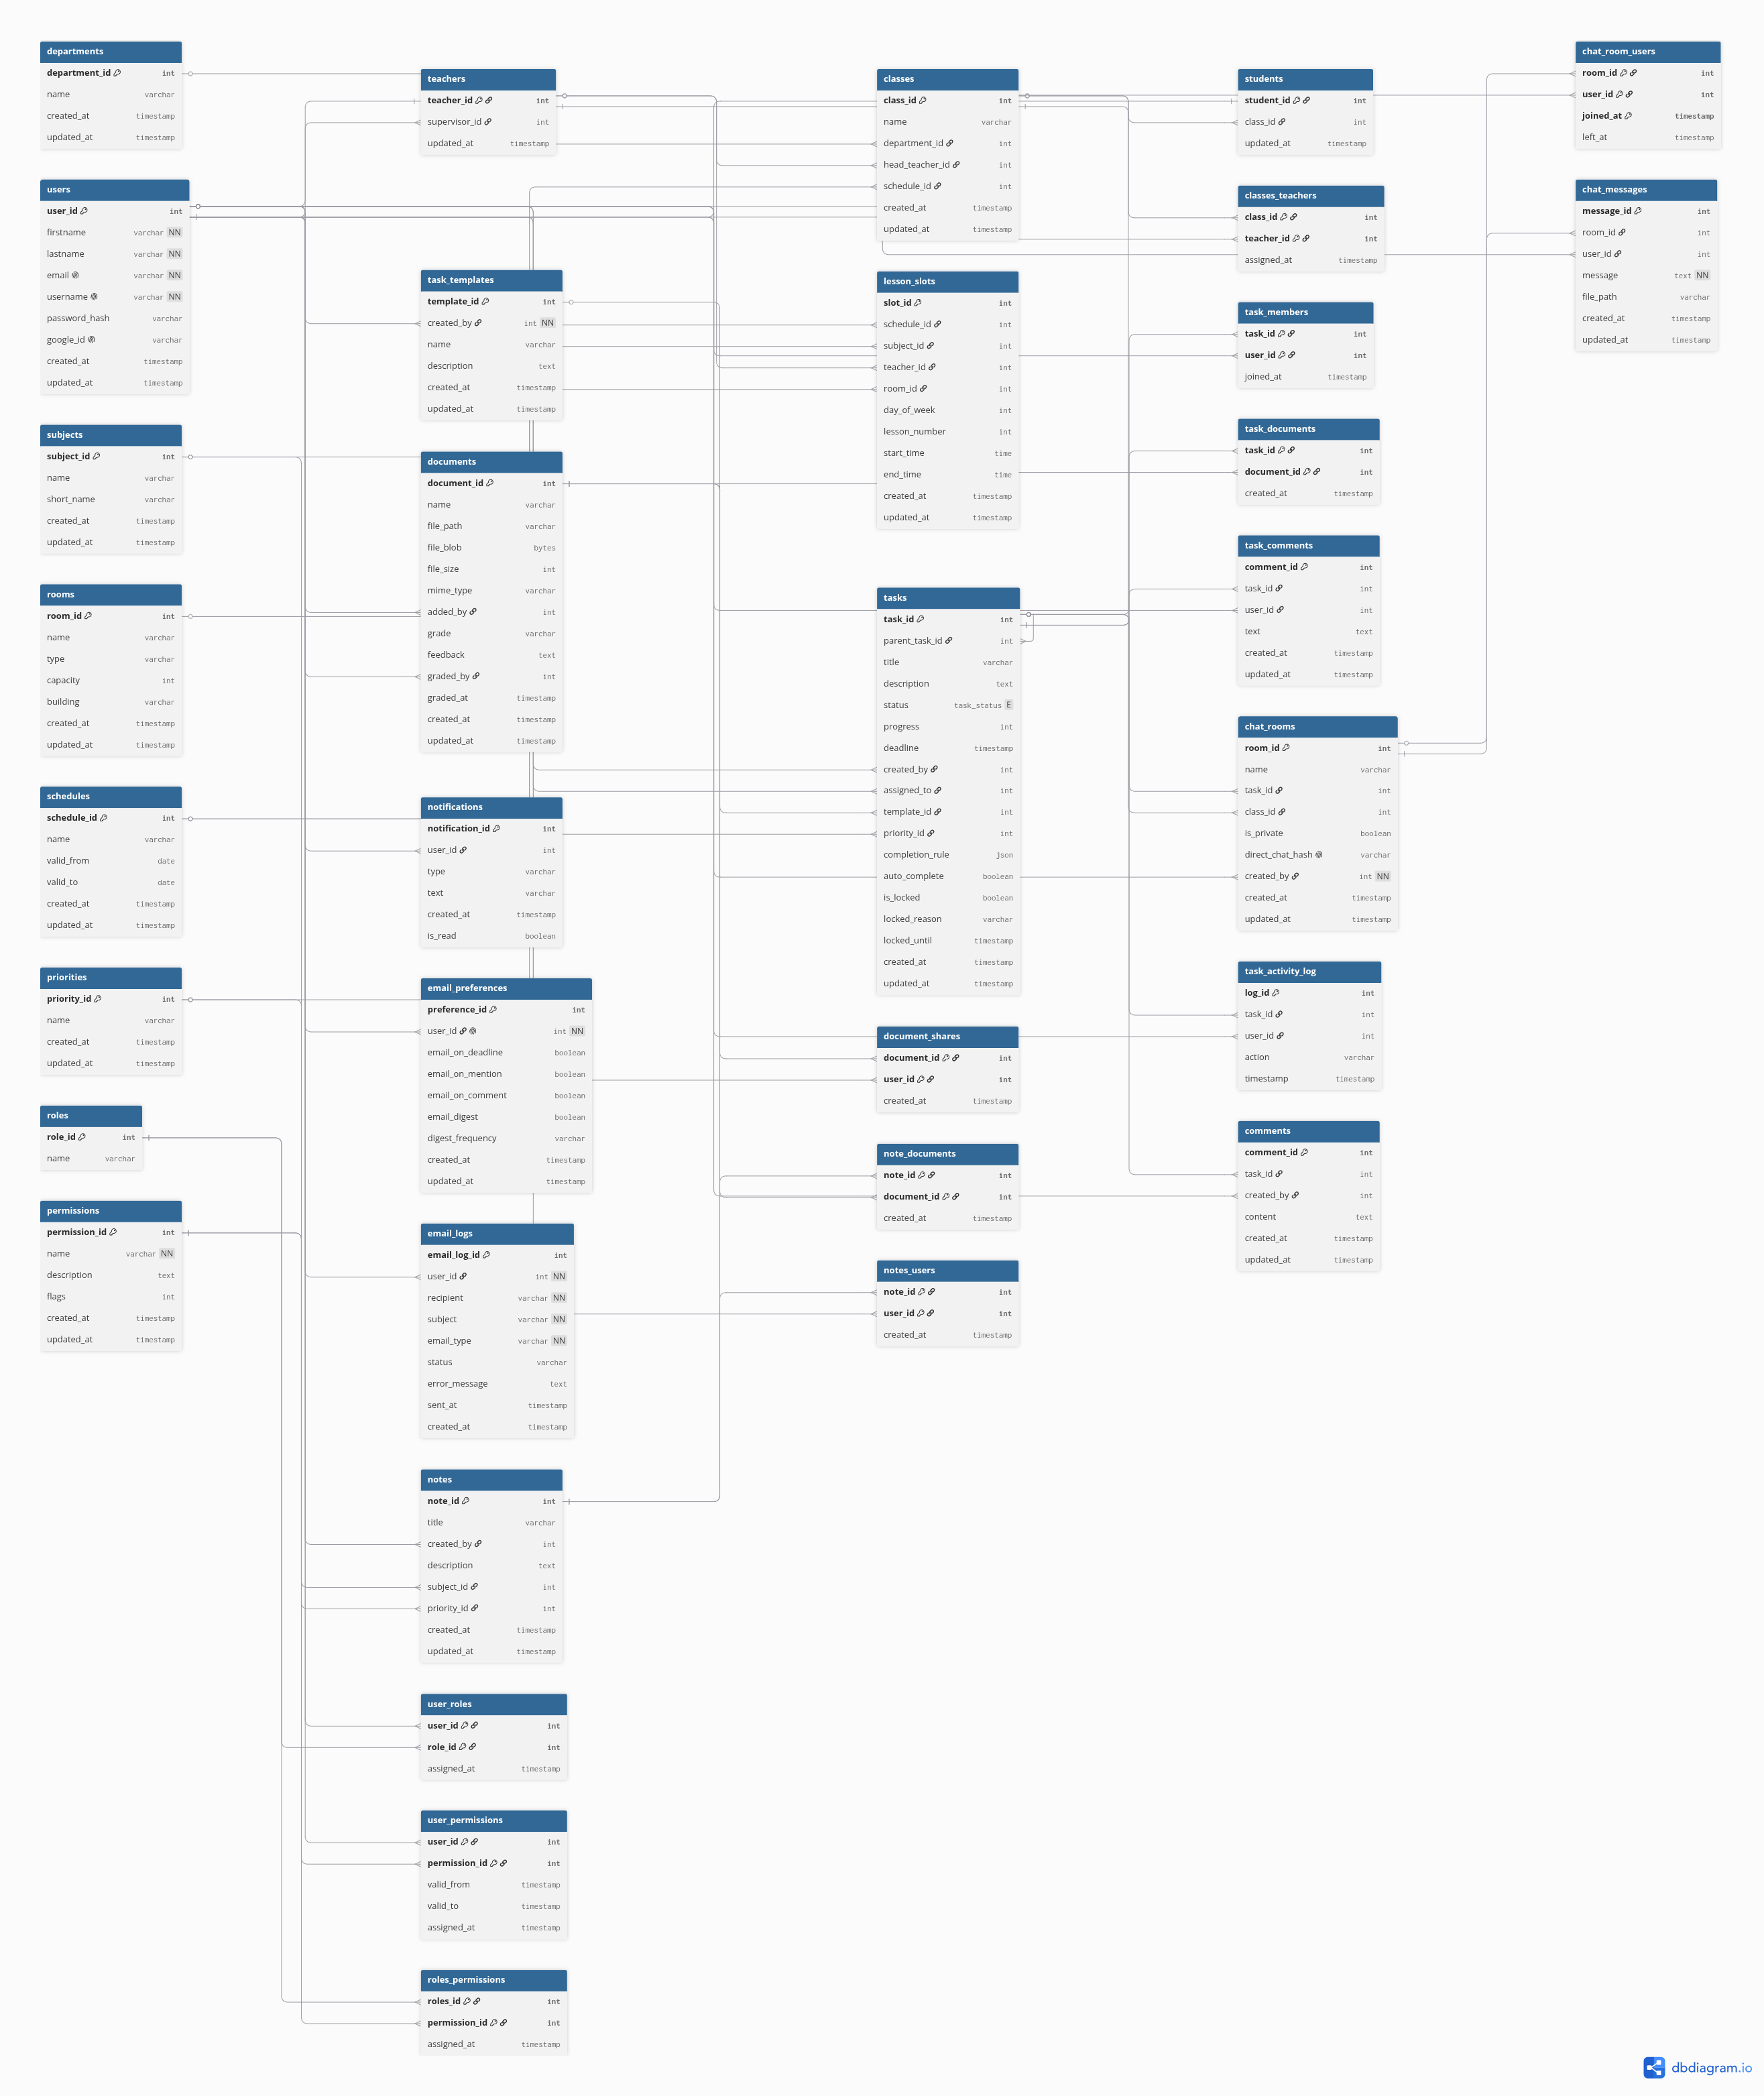
\includegraphics[width=\textwidth, height=\textheight, keepaspectratio]{content/bilder/Untitled.png}
    \caption{Vollständiges Entity-Relationship-Diagramm von EffSync}
    \label{fig:erd_vollstaendig}
\end{figure}

% ─────────────────────────────────────────────────────────────
\clearpage
\section{Fragebogen und Rohdaten des Usability-Tests}
\label{sec:anhang_usability}

Dieser Abschnitt enthält den vollständigen Aufgabenkatalog sowie die erhobenen
Rohdaten (Bearbeitungszeiten, Beobachtungsnotizen) des in
Abschnitt~\ref{sec:usability_test} beschriebenen Usability-Tests.


\subsection*{Effsync Usability-Test v2 (30 Minuten)}

\noindent
\textbf{Repository:} \url{https://github.com/kiDra94/diplom-arbeit} \\
\textbf{Datum:} \underline{\hspace{4cm}} \quad
\textbf{Testleitung:} \underline{\hspace{4cm}} \quad
\textbf{Test-ID:} \underline{\hspace{3cm}} \\
\textbf{Teilnehmer-Rolle:} $\square$ Schüler \quad $\square$ Lehrer \quad $\square$ Admin \\
\textbf{Browser A:} \underline{\hspace{3cm}} \quad
\textbf{Browser B:} \underline{\hspace{3cm}}

% ─────────────────────────────────────────────────────────────
\subsection*{1) Ablauf (für Testleitung)}

\begin{itemize}
    \item Intro: 2 Min
    \item Warm-up: 3 Min
    \item Szenario 1: 6 Min
    \item Szenario 2: 6 Min
    \item Szenario 3: 6 Min
    \item Cross-Browser-Chat: 5 Min
    \item Abschlussfragen: 2 Min
\end{itemize}

\noindent\textbf{Regel:} Nicht helfen, außer wenn Teilnehmer komplett feststeckt (nach ca. 90 Sek).

% ─────────────────────────────────────────────────────────────
\subsection*{2) Aufgabenblatt (Teilnehmer + Beobachtung)}

\subsubsection*{Aufgabe 1 – Orientierung unter Zeitdruck (6 Min)}

\noindent\textbf{Ziel (rollenabhängig):}
\begin{itemize}
    \item Schüler: letzte Aufgabe + Abgabedatum finden
    \item Lehrer: Stelle finden, um neue Aufgabe zu veröffentlichen
    \item Admin: Stelle finden, um Rollen/Rechte zu ändern
\end{itemize}

\noindent\textbf{Messung:} \\
Startzeit: \underline{\hspace{2cm}} \quad
Endzeit: \underline{\hspace{2cm}} \quad
Dauer: \underline{\hspace{2cm}} \\
Erfolg: $\square$ Ja \quad $\square$ Teilweise \quad $\square$ Nein \\
Fehlklicks/Sackgassen: \underline{\hspace{3cm}}

\noindent\textbf{Kommentar (Beobachtung + Verbesserungsvorschläge):}

\vspace{2cm}
\noindent\rule{\textwidth}{0.4pt}

% ─────────────────────────────────────────────────────────────
\subsubsection*{Aufgabe 2 – Kritischer Hauptflow (6 Min)}

\noindent\textbf{Ziel (rollenabhängig):}
\begin{itemize}
    \item Schüler: Kernaufgabe vollständig durchführen
    \item Lehrer: Aufgabe erstellen und sichtbares Ergebnis prüfen
    \item Admin: Rollenänderung durchführen und Berechtigung prüfen
\end{itemize}

\noindent\textbf{Messung:} \\
Startzeit: \underline{\hspace{2cm}} \quad
Endzeit: \underline{\hspace{2cm}} \quad
Dauer: \underline{\hspace{2cm}} \\
Erfolg: $\square$ Ja \quad $\square$ Teilweise \quad $\square$ Nein \\
Hilfe nötig: $\square$ Nein \quad $\square$ Ja, kurz \quad $\square$ Ja, stark

\noindent\textbf{Kommentar (Beobachtung + Verbesserungsvorschläge):}

\vspace{2cm}
\noindent\rule{\textwidth}{0.4pt}

% ─────────────────────────────────────────────────────────────
\subsubsection*{Aufgabe 3 – Fehlerfall / Recovery (6 Min)}

\noindent\textbf{Ziel:} Nach absichtlichem Fehlweg wieder korrekt zur Aufgabe zurückfinden.

\noindent\textbf{Messung:} \\
Startzeit: \underline{\hspace{2cm}} \quad
Endzeit: \underline{\hspace{2cm}} \quad
Dauer: \underline{\hspace{2cm}} \\
Recovery geschafft: $\square$ Ja \quad $\square$ Teilweise \quad $\square$ Nein \\
Strategie genutzt: $\square$ Zurück \quad $\square$ Menü \quad $\square$ Suche \quad
$\square$ Sonstiges: \underline{\hspace{2cm}}

\noindent\textbf{Kommentar (Beobachtungen + Verbesserungsvorschläge):}

\vspace{2cm}
\noindent\rule{\textwidth}{0.4pt}

% ─────────────────────────────────────────────────────────────
\subsubsection*{Aufgabe 4 – Cross-Browser Chat-Test (5 Min)}

\noindent\textbf{Setup:} \\
Browser A (z.\,B. Chrome): Rolle \underline{\hspace{3cm}} \\
Browser B (z.\,B. Firefox): Rolle \underline{\hspace{3cm}}

\noindent\textbf{Checks:}
\begin{enumerate}
    \item A $\rightarrow$ B Nachricht zugestellt: $\square$ Ja \quad $\square$ Nein \quad Zeit: \underline{\hspace{1cm}} Sek
    \item B $\rightarrow$ A Nachricht zugestellt: $\square$ Ja \quad $\square$ Nein \quad Zeit: \underline{\hspace{1cm}} Sek
    \item Gleichzeitiges Senden korrekt: $\square$ Ja \quad $\square$ Nein
    \item Nach Reload bleibt Verlauf korrekt: $\square$ Ja \quad $\square$ Nein
    \item Reihenfolge/Zeitstempel konsistent: $\square$ Ja \quad $\square$ Nein
\end{enumerate}

\noindent\textbf{Kommentar (Beobachtungen + Verbesserungsvorschläge):}

\vspace{2cm}
\noindent\rule{\textwidth}{0.4pt}

% ─────────────────────────────────────────────────────────────
\subsection*{3) Abschluss (2 Min) – Teilnehmer}

\noindent\textbf{Bitte auf Skala 1 (trifft gar nicht zu) bis 7 (trifft voll zu):}

\bigskip
\noindent 1. Ich konnte meine wichtigsten Aufgaben schnell erledigen. \\
$\square$\,1 \quad $\square$\,2 \quad $\square$\,3 \quad $\square$\,4 \quad $\square$\,5 \quad $\square$\,6 \quad $\square$\,7

\bigskip
\noindent 2. Ich wusste jederzeit, wo ich bin und was ich als Nächstes tun kann. \\
$\square$\,1 \quad $\square$\,2 \quad $\square$\,3 \quad $\square$\,4 \quad $\square$\,5 \quad $\square$\,6 \quad $\square$\,7

\bigskip
\noindent 3. Bei Fehlern konnte ich mich leicht erholen. \\
$\square$\,1 \quad $\square$\,2 \quad $\square$\,3 \quad $\square$\,4 \quad $\square$\,5 \quad $\square$\,6 \quad $\square$\,7

\bigskip
\noindent 4. Ich vertraue dem Chat (Zustellung/Reihenfolge). \\
$\square$\,1 \quad $\square$\,2 \quad $\square$\,3 \quad $\square$\,4 \quad $\square$\,5 \quad $\square$\,6 \quad $\square$\,7

\bigskip
\noindent\textbf{Was hat dich am meisten frustriert?} \\
\vspace{2cm}
\noindent\rule{\textwidth}{0.4pt}

\bigskip
\noindent\textbf{Welche eine Verbesserung hätte den größten Effekt?} \\
\vspace{2cm}
\noindent\rule{\textwidth}{0.4pt}

% ─────────────────────────────────────────────────────────────
\subsection*{4) Auswertung (Testleitung, nach Session)}

\noindent\textbf{Top-Probleme (max. 3):}
\begin{enumerate}
    \item \underline{\hspace{8cm}} (Priorität: P1 / P2 / P3)
    \item \underline{\hspace{8cm}} (Priorität: P1 / P2 / P3)
    \item \underline{\hspace{8cm}} (Priorität: P1 / P2 / P3)
\end{enumerate}

\noindent\textbf{Kurzfazit (1–2 Sätze):} \\
\vspace{2cm}
\noindent\rule{\textwidth}{0.4pt}
     
% ─────────────────────────────────────────────────────────────
\clearpage
\section{Auszug aus dem Prisma-Datenbankschema}
\label{sec:anhang_prisma}

Der folgende Auszug zeigt alle relevanten Modelle aus der Datei \texttt{schema.prisma},
die das vollständige Datenbankschema von EffSync abbilden.

% ── Generator & Datasource ──────────────────────────────────
\begin{listing}[H]
\begin{minted}[fontsize=\small, breaklines]{text}
generator client {
  provider     = "prisma-client-js"
  moduleFormat = "cjs"
  engineType   = "library"
}

datasource db {
  provider = "postgresql"
}
\end{minted}
\caption{Prisma -- Generator und Datasource}
\label{lst:prisma_generator}
\end{listing}

% ── Enums ───────────────────────────────────────────────────
\begin{listing}[H]
\begin{minted}[fontsize=\small, breaklines]{text}
enum user_role {
  Superuser
  Admin
  Teacher
  Student
}

enum task_status {
  TODO
  IN_PROGRESS
  IN_REVIEW
  ON_HOLD
  COMPLETED
}
\end{minted}
\caption{Prisma -- Enumerationen \texttt{user\_role} und \texttt{task\_status}}
\label{lst:prisma_enums}
\end{listing}

% ── Users ───────────────────────────────────────────────────
\begin{listing}[H]
\begin{minted}[fontsize=\small, breaklines]{text}
model users {
  user_id                                Int                 @id @default(autoincrement())
  firstname                              String              @db.VarChar
  lastname                               String              @db.VarChar
  email                                  String              @unique @db.VarChar
  username                               String              @unique @db.VarChar
  password_hash                          String?             @db.VarChar
  google_id                              String?             @unique @db.VarChar
  created_at                             DateTime?           @default(now()) @db.Timestamp(6)
  updated_at                             DateTime?           @updatedAt @db.Timestamp(6)
  chat_messages                          chat_messages[]
  chat_room_users                        chat_room_users[]
  document_shares                        document_shares[]
  documents                              documents[]
  graded_documents                       documents[]         @relation("documents_graded_by")
  notes                                  notes[]
  notes_users                            notes_users[]
  notifications                          notifications[]
  comments                               comments[]
  email_preferences                      email_preferences?
  email_logs                             email_logs[]
  students                               students?
  task_activity_log                      task_activity_log[]
  task_comments                          task_comments[]
  tasks_tasks_assigned_toTousers         tasks[]             @relation("tasks_assigned_toTousers")
  tasks_tasks_created_byTousers          tasks[]             @relation("tasks_created_byTousers")
  teachers_teachers_supervisor_idTousers teachers[]          @relation("teachers_supervisor_idTousers")
  teachers_teachers_teacher_idTousers    teachers?           @relation("teachers_teacher_idTousers")
  user_permissions                       user_permissions[]
  user_roles                             user_roles[]
  taskTemplates                          task_templates[]
  task_members                           task_members[]
  chat_rooms_created                     chat_rooms[]        @relation("chat_rooms_created")
}

model teachers {
  teacher_id                          Int                @id
  supervisor_id                       Int?
  updated_at                          DateTime?          @db.Timestamp(6)
  classes                             classes[]
  classes_teachers                    classes_teachers[]
  lesson_slots                        lesson_slots[]
  users_teachers_supervisor_idTousers users?             @relation("teachers_supervisor_idTousers", fields: [supervisor_id], references: [user_id], onDelete: NoAction, onUpdate: NoAction)
  users_teachers_teacher_idTousers    users              @relation("teachers_teacher_idTousers", fields: [teacher_id], references: [user_id], onDelete: NoAction, onUpdate: NoAction)
}

model students {
  student_id Int       @id
  class_id   Int?
  updated_at DateTime? @db.Timestamp(6)
  classes    classes?  @relation(fields: [class_id], references: [class_id], onDelete: NoAction, onUpdate: NoAction)
  users      users     @relation(fields: [student_id], references: [user_id], onDelete: NoAction, onUpdate: NoAction)
}
\end{minted}
\caption{Prisma -- Modell \texttt{users} sowie die spezialisierten Rollen \texttt{teachers} und \texttt{students}}
\label{lst:prisma_users}
\end{listing}

% ── Organisation: Departments, Classes, Subjects, Rooms, Schedules ──
\begin{listing}[H]
\begin{minted}[fontsize=\small, breaklines]{text}
model departments {
  department_id Int       @id @default(autoincrement())
  name          String?   @db.VarChar
  created_at    DateTime? @default(now()) @db.Timestamp(6)
  updated_at    DateTime? @db.Timestamp(6)
  classes       classes[]
}

model classes {
  class_id         Int                @id @default(autoincrement())
  name             String?            @db.VarChar
  department_id    Int?
  head_teacher_id  Int?
  schedule_id      Int?
  created_at       DateTime?          @default(now()) @db.Timestamp(6)
  updated_at       DateTime?          @db.Timestamp(6)
  chat_rooms       chat_rooms[]
  departments      departments?       @relation(fields: [department_id], references: [department_id], onDelete: NoAction, onUpdate: NoAction)
  teachers         teachers?          @relation(fields: [head_teacher_id], references: [teacher_id], onDelete: NoAction, onUpdate: NoAction)
  schedules        schedules?         @relation(fields: [schedule_id], references: [schedule_id], onDelete: NoAction, onUpdate: NoAction)
  classes_teachers classes_teachers[]
  students         students[]
}

model classes_teachers {
  class_id    Int
  teacher_id  Int
  assigned_at DateTime? @default(now()) @db.Timestamp(6)
  classes     classes   @relation(fields: [class_id], references: [class_id], onDelete: NoAction, onUpdate: NoAction)
  teachers    teachers  @relation(fields: [teacher_id], references: [teacher_id], onDelete: NoAction, onUpdate: NoAction)

  @@id([class_id, teacher_id])
}

model subjects {
  subject_id   Int            @id @default(autoincrement())
  name         String?        @db.VarChar
  short_name   String?        @db.VarChar
  created_at   DateTime?      @default(now()) @db.Timestamp(6)
  updated_at   DateTime?      @db.Timestamp(6)
  lesson_slots lesson_slots[]
  notes        notes[]
}

model rooms {
  room_id      Int            @id @default(autoincrement())
  name         String?        @db.VarChar
  type         String?        @db.VarChar
  capacity     Int?
  building     String?        @db.VarChar
  created_at   DateTime?      @default(now()) @db.Timestamp(6)
  updated_at   DateTime?      @db.Timestamp(6)
  lesson_slots lesson_slots[]
}

model schedules {
  schedule_id  Int            @id @default(autoincrement())
  name         String?        @db.VarChar
  valid_from   DateTime?      @db.Date
  valid_to     DateTime?      @db.Date
  created_at   DateTime?      @default(now()) @db.Timestamp(6)
  updated_at   DateTime?      @db.Timestamp(6)
  classes      classes[]
  lesson_slots lesson_slots[]
}

model lesson_slots {
  slot_id       Int        @id @default(autoincrement())
  schedule_id   Int?
  subject_id    Int?
  teacher_id    Int?
  room_id       Int?
  day_of_week   Int?
  lesson_number Int?
  start_time    DateTime?  @db.Time(6)
  end_time      DateTime?  @db.Time(6)
  created_at    DateTime?  @default(now()) @db.Timestamp(6)
  updated_at    DateTime?  @db.Timestamp(6)
  rooms         rooms?     @relation(fields: [room_id], references: [room_id], onDelete: NoAction, onUpdate: NoAction)
  schedules     schedules? @relation(fields: [schedule_id], references: [schedule_id], onDelete: NoAction, onUpdate: NoAction)
  subjects      subjects?  @relation(fields: [subject_id], references: [subject_id], onDelete: NoAction, onUpdate: NoAction)
  teachers      teachers?  @relation(fields: [teacher_id], references: [teacher_id], onDelete: NoAction, onUpdate: NoAction)
}
\end{minted}
\caption{Prisma -- Organisationsmodelle (Departments, Klassen, Fächer, Räume, Stundenpläne)}
\label{lst:prisma_organisation}
\end{listing}

% ── Rollen & Berechtigungen (RBAC) ─────────────────────────────────
\begin{listing}[H]
\begin{minted}[fontsize=\small, breaklines]{text}
model roles {
  role_id           Int                 @id @default(autoincrement())
  name              String?             @db.VarChar
  roles_permissions roles_permissions[]
  user_roles        user_roles[]
}

model permissions {
  permission_id     Int                 @id @default(autoincrement())
  name              String              @db.VarChar          // z.B. 'create_task', 'edit_grades'
  description       String?
  flags             Int                 @default(7)          // 4=READ, 2=WRITE, 1=EXECUTE (7=RWX)
  created_at        DateTime?           @default(now()) @db.Timestamp(6)
  updated_at        DateTime?           @updatedAt @db.Timestamp(6)
  roles_permissions roles_permissions[]
  user_permissions  user_permissions[]
}

model roles_permissions {
  roles_id      Int
  permission_id Int
  assigned_at   DateTime?   @default(now()) @db.Timestamp(6)
  permissions   permissions @relation(fields: [permission_id], references: [permission_id], onDelete: NoAction, onUpdate: NoAction)
  roles         roles       @relation(fields: [roles_id], references: [role_id], onDelete: NoAction, onUpdate: NoAction)

  @@id([roles_id, permission_id])
}

model user_roles {
  user_id     Int
  role_id     Int
  assigned_at DateTime? @default(now()) @db.Timestamp(6)
  roles       roles     @relation(fields: [role_id], references: [role_id], onDelete: NoAction, onUpdate: NoAction)
  users       users     @relation(fields: [user_id], references: [user_id], onDelete: NoAction, onUpdate: NoAction)

  @@id([user_id, role_id])
}

model user_permissions {
  user_id       Int
  permission_id Int
  valid_from    DateTime?   @default(now()) @db.Timestamp(6)  // Wann die Permission startet
  valid_to      DateTime?                   @db.Timestamp(6)  // Wann die Permission ENDET (null=unbegrenzt)
  assigned_at   DateTime?   @default(now()) @db.Timestamp(6)
  permissions   permissions @relation(fields: [permission_id], references: [permission_id], onDelete: Cascade, onUpdate: NoAction)
  users         users       @relation(fields: [user_id], references: [user_id], onDelete: Cascade, onUpdate: NoAction)

  @@id([user_id, permission_id])
  @@index([valid_from, valid_to])  // Für schnelle Zeitabfragen
}
\end{minted}
\caption{Prisma -- Rollen- und Berechtigungsmodelle (RBAC)}
\label{lst:prisma_rbac}
\end{listing}

% ── Tasks ───────────────────────────────────────────────────
\begin{listing}[H]
\begin{minted}[fontsize=\small, breaklines]{text}
model tasks {
  task_id                        Int                 @id @default(autoincrement())
  parent_task_id                 Int?
  title                          String?             @db.VarChar
  description                    String?
  status                         task_status?        @default(TODO)
  progress                       Int?
  deadline                       DateTime?           @db.Timestamp(6)
  created_by                     Int?
  assigned_to                    Int?
  template_id                    Int?
  priority_id                    Int?
  completion_rule                Json?
  auto_complete                  Boolean?
  is_locked                      Boolean?            @default(false)
  locked_reason                  String?             @db.VarChar
  locked_until                   DateTime?           @db.Timestamp(6)
  created_at                     DateTime?           @default(now()) @db.Timestamp(6)
  updated_at                     DateTime?           @updatedAt @db.Timestamp(6)
  chat_rooms                     chat_rooms[]
  task_activity_log              task_activity_log[]
  task_comments                  task_comments[]
  task_documents                 task_documents[]
  task_members                   task_members[]
  comments                       comments[]
  users_tasks_assigned_toTousers users?              @relation("tasks_assigned_toTousers", fields: [assigned_to], references: [user_id], onDelete: NoAction, onUpdate: NoAction)
  users_tasks_created_byTousers  users?              @relation("tasks_created_byTousers", fields: [created_by], references: [user_id], onDelete: NoAction, onUpdate: NoAction)
  tasks                          tasks?              @relation("tasksTotasks", fields: [parent_task_id], references: [task_id], onDelete: NoAction, onUpdate: NoAction)
  other_tasks                    tasks[]             @relation("tasksTotasks")
  priorities                     priorities?         @relation(fields: [priority_id], references: [priority_id], onDelete: NoAction, onUpdate: NoAction)
  task_templates                 task_templates?     @relation(fields: [template_id], references: [template_id], onDelete: NoAction, onUpdate: NoAction)
}

model task_templates {
  template_id Int       @id @default(autoincrement())
  created_by  Int
  name        String?   @db.VarChar
  description String?
  created_at  DateTime? @default(now()) @db.Timestamp(6)
  updated_at  DateTime? @db.Timestamp(6)
  user        users     @relation(fields: [created_by], references: [user_id])
  tasks       tasks[]
}

model task_members {
  task_id   Int
  user_id   Int
  joined_at DateTime @default(now()) @db.Timestamp(6)
  tasks     tasks    @relation(fields: [task_id], references: [task_id], onDelete: Cascade)
  users     users    @relation(fields: [user_id], references: [user_id], onDelete: Cascade)

  @@id([task_id, user_id])
}

model priorities {
  priority_id Int       @id @default(autoincrement())
  name        String?
  created_at  DateTime? @default(now()) @db.Timestamp(6)
  updated_at  DateTime? @db.Timestamp(6)
  notes       notes[]
  tasks       tasks[]
}

model task_documents {
  task_id     Int
  document_id Int
  created_at  DateTime? @default(now()) @db.Timestamp(6)
  documents   documents @relation(fields: [document_id], references: [document_id], onDelete: NoAction, onUpdate: NoAction)
  tasks       tasks     @relation(fields: [task_id], references: [task_id], onDelete: NoAction, onUpdate: NoAction)

  @@id([task_id, document_id])
}

model task_comments {
  comment_id Int       @id @default(autoincrement())
  task_id    Int?
  user_id    Int?
  text       String?
  created_at DateTime? @default(now()) @db.Timestamp(6)
  updated_at DateTime? @db.Timestamp(6)
  tasks      tasks?    @relation(fields: [task_id], references: [task_id], onDelete: NoAction, onUpdate: NoAction)
  users      users?    @relation(fields: [user_id], references: [user_id], onDelete: NoAction, onUpdate: NoAction)
}

model comments {
  comment_id Int       @id @default(autoincrement())
  task_id    Int?
  created_by Int?
  content    String?
  created_at DateTime? @default(now()) @db.Timestamp(6)
  updated_at DateTime? @db.Timestamp(6)
  users      users?    @relation(fields: [created_by], references: [user_id], onDelete: NoAction, onUpdate: NoAction)
  tasks      tasks?    @relation(fields: [task_id], references: [task_id], onDelete: NoAction, onUpdate: NoAction)
}

model task_activity_log {
  log_id    Int       @id @default(autoincrement())
  task_id   Int?
  user_id   Int?
  action    String?   @db.VarChar
  timestamp DateTime? @default(now()) @db.Timestamp(6)
  tasks     tasks?    @relation(fields: [task_id], references: [task_id], onDelete: NoAction, onUpdate: NoAction)
  users     users?    @relation(fields: [user_id], references: [user_id], onDelete: NoAction, onUpdate: NoAction)
}
\end{minted}
\caption{Prisma -- Aufgaben-Modelle (\texttt{tasks}, \texttt{task\_members}, \texttt{task\_templates} u.\,w.)}
\label{lst:prisma_tasks}
\end{listing}

% ── Dokumente & Notizen ─────────────────────────────────────
\begin{listing}[H]
\begin{minted}[fontsize=\small, breaklines]{text}
model documents {
  document_id     Int               @id @default(autoincrement())
  name            String?           @db.VarChar
  file_path       String?           @db.VarChar
  file_blob       Bytes?
  file_size       Int?
  mime_type       String?           @db.VarChar
  added_by        Int?
  grade           String?           @db.VarChar
  feedback        String?
  graded_by       Int?
  graded_at       DateTime?         @db.Timestamp(6)
  created_at      DateTime?         @default(now()) @db.Timestamp(6)
  updated_at      DateTime?         @db.Timestamp(6)
  document_shares document_shares[]
  graded_by_user  users?            @relation("documents_graded_by", fields: [graded_by], references: [user_id], onDelete: NoAction, onUpdate: NoAction)
  users           users?            @relation(fields: [added_by], references: [user_id], onDelete: NoAction, onUpdate: NoAction)
  note_documents  note_documents[]
  task_documents  task_documents[]
}

model document_shares {
  document_id Int
  user_id     Int
  created_at  DateTime? @default(now()) @db.Timestamp(6)
  documents   documents @relation(fields: [document_id], references: [document_id], onDelete: NoAction, onUpdate: NoAction)
  users       users     @relation(fields: [user_id], references: [user_id], onDelete: NoAction, onUpdate: NoAction)

  @@id([document_id, user_id])
}

model notes {
  note_id        Int              @id @default(autoincrement())
  title          String?          @db.VarChar
  created_by     Int?
  description    String?
  subject_id     Int?
  priority_id    Int?
  created_at     DateTime?        @default(now()) @db.Timestamp(6)
  updated_at     DateTime?        @db.Timestamp(6)
  note_documents note_documents[]
  users          users?           @relation(fields: [created_by], references: [user_id], onDelete: NoAction, onUpdate: NoAction)
  priorities     priorities?      @relation(fields: [priority_id], references: [priority_id], onDelete: NoAction, onUpdate: NoAction)
  subjects       subjects?        @relation(fields: [subject_id], references: [subject_id], onDelete: NoAction, onUpdate: NoAction)
  notes_users    notes_users[]
}

model note_documents {
  note_id     Int
  document_id Int
  created_at  DateTime? @default(now()) @db.Timestamp(6)
  documents   documents @relation(fields: [document_id], references: [document_id], onDelete: NoAction, onUpdate: NoAction)
  notes       notes     @relation(fields: [note_id], references: [note_id], onDelete: NoAction, onUpdate: NoAction)

  @@id([note_id, document_id])
}

model notes_users {
  note_id    Int
  user_id    Int
  created_at DateTime? @default(now()) @db.Timestamp(6)
  notes      notes     @relation(fields: [note_id], references: [note_id], onDelete: NoAction, onUpdate: NoAction)
  users      users     @relation(fields: [user_id], references: [user_id], onDelete: NoAction, onUpdate: NoAction)

  @@id([note_id, user_id])
}
\end{minted}
\caption{Prisma -- Dokumenten- und Notizmodelle}
\label{lst:prisma_documents_notes}
\end{listing}

% ── Kommunikation: Chat & Benachrichtigungen ────────────────
\begin{listing}[H]
\begin{minted}[fontsize=\small, breaklines]{text}
model chat_rooms {
  room_id          Int               @id @default(autoincrement())
  name             String?           @db.VarChar
  task_id          Int?
  class_id         Int?
  is_private       Boolean           @default(false)
  direct_chat_hash String?           @unique @db.VarChar(50)
  created_by       Int
  created_at       DateTime          @default(now()) @db.Timestamp(6)
  updated_at       DateTime?         @updatedAt @db.Timestamp(6)
  chat_messages    chat_messages[]
  chat_room_users  chat_room_users[]
  classes          classes?          @relation(fields: [class_id], references: [class_id], onDelete: NoAction, onUpdate: NoAction)
  tasks            tasks?            @relation(fields: [task_id], references: [task_id], onDelete: NoAction, onUpdate: NoAction)
  users            users?            @relation("chat_rooms_created", fields: [created_by], references: [user_id], onDelete: NoAction, onUpdate: NoAction)
}

model chat_room_users {
  room_id    Int
  user_id    Int
  joined_at  DateTime   @default(now()) @db.Timestamp(6)
  left_at    DateTime?  @db.Timestamp(6)
  chat_rooms chat_rooms @relation(fields: [room_id], references: [room_id], onDelete: NoAction, onUpdate: NoAction)
  users      users      @relation(fields: [user_id], references: [user_id], onDelete: NoAction, onUpdate: NoAction)

  @@id([room_id, user_id, joined_at])
}

model chat_messages {
  message_id Int         @id @default(autoincrement())
  room_id    Int
  user_id    Int
  message    String
  file_path  String?     @db.VarChar
  created_at DateTime    @default(now()) @db.Timestamp(6)
  updated_at DateTime?   @updatedAt @db.Timestamp(6)
  chat_rooms chat_rooms? @relation(fields: [room_id], references: [room_id], onDelete: NoAction, onUpdate: NoAction)
  users      users?      @relation(fields: [user_id], references: [user_id], onDelete: NoAction, onUpdate: NoAction)
}

model notifications {
  notification_id Int       @id @default(autoincrement())
  user_id         Int?
  type            String?   @db.VarChar
  text            String?   @db.VarChar
  created_at      DateTime? @default(now()) @db.Timestamp(6)
  is_read         Boolean?  @default(false)
  users           users?    @relation(fields: [user_id], references: [user_id], onDelete: NoAction, onUpdate: NoAction)
}
\end{minted}
\caption{Prisma -- Chat- und Benachrichtigungsmodelle}
\label{lst:prisma_chat}
\end{listing}

% ── E-Mail ──────────────────────────────────────────────────
\begin{listing}[H]
\begin{minted}[fontsize=\small, breaklines]{text}
model email_preferences {
  preference_id     Int       @id @default(autoincrement())
  user_id           Int       @unique
  email_on_deadline Boolean   @default(true)
  email_on_mention  Boolean   @default(true)
  email_on_comment  Boolean   @default(true)
  email_digest      Boolean   @default(false)
  digest_frequency  String    @default("daily") @db.VarChar // daily, weekly, monthly
  created_at        DateTime? @default(now()) @db.Timestamp(6)
  updated_at        DateTime? @updatedAt @db.Timestamp(6)
  users             users     @relation(fields: [user_id], references: [user_id], onDelete: Cascade)
}

model email_logs {
  email_log_id  Int       @id @default(autoincrement())
  user_id       Int
  recipient     String    @db.VarChar
  subject       String    @db.VarChar
  email_type    String    @db.VarChar // 'deadline', 'mention', 'comment', 'digest'
  status        String    @default("sent") @db.VarChar // 'sent', 'failed', 'pending'
  error_message String?   @db.Text
  sent_at       DateTime? @db.Timestamp(6)
  created_at    DateTime? @default(now()) @db.Timestamp(6)
  users         users     @relation(fields: [user_id], references: [user_id], onDelete: Cascade)
}
\end{minted}
\caption{Prisma -- E-Mail-Modelle}
\label{lst:prisma_email}
\end{listing}  % ← TODO ersetzen durch das

% ─────────────────────────────────────────────────────────────


    % ---> NEU: Hier wird die Autoren-Tabelle ausgegeben
    \chapter*{Übersicht der Autorinnen und Autoren}
    \addcontentsline{toc}{chapter}{Übersicht der Autorinnen und Autoren}

    \begin{longtable}{p{2cm} p{8cm} p{4cm}}
    \textbf{Kapitel} & \textbf{Titel} & \textbf{Autor*in} \\
    \hline
    \hline
    \endfirsthead
    \textbf{Kapitel} & \textbf{Titel} & \textbf{Autor*in} \\
    \hline
    \endhead
    % Inhalt wird aus dem Speicher geladen:
    \authorlist
    \end{longtable}
    % <---
    

% \end{singlespace}
\printglossaries
\printbibliography
\end{document}